\documentclass[12pt,a4paper]{article}

% --- Packages ---
\usepackage[margin=2.5cm]{geometry}
\usepackage{graphicx}
\usepackage{booktabs}
\usepackage{tabularx}
\usepackage{amsmath}
\usepackage{amsthm}
\usepackage{amssymb}
\usepackage{hyperref}
\usepackage{caption}
\usepackage{subcaption}
\usepackage{float}
\usepackage{enumitem}
\usepackage{longtable}
\usepackage{xcolor}
\usepackage{natbib}
\usepackage{microtype}
\usepackage{setspace}
\usepackage{tikz}
\usepackage{array}
\usepackage{bm}
\usetikzlibrary{shapes.geometric,arrows.meta,positioning}

% --- Fix: define C column type for tabularx ---
\newcolumntype{C}{>{\centering\arraybackslash}X}

\newtheorem{theorem}{Theorem}[section]
\newtheorem{lemma}[theorem]{Lemma}
\newtheorem{proposition}[theorem]{Proposition}
\newtheorem{corollary}[theorem]{Corollary}
\newtheorem{definition}[theorem]{Definition}
\newtheorem{remark}[theorem]{Remark}

% --- Document Formatting ---
\onehalfspacing
\hypersetup{
    colorlinks=false,
    pdfborder={0 0 0},
    pdftitle={The Great Divergence: When Machines Hallucinate and Humans Still See},
    pdfauthor={Mina Magdy, Sandy Antonius, Youssef Ayman Mahmoud, Eyad Saleh Ali, Mariam Mohammed}
}

\title{\textbf{The Great Divergence: When Machines Hallucinate and Humans Still See}\\[6pt]
\large Bridging the Biological Gap with Recurrent Predictive Coding,\\
Spherical Decision Geometry, and Active Inference}

\author{
    Mina Magdy\textsuperscript{1} \quad
    Sandy Antonius\textsuperscript{1} \quad
    Youssef Ayman Mahmoud\textsuperscript{1} \\[4pt]
    Eyad Saleh Ali\textsuperscript{1} \quad
    Mariam Mohammed\textsuperscript{1} \\[8pt]
    \small\textsuperscript{1}Sadat Academy for Management Sciences,
    AI Department, Year~3
}

\date{\small\today}

\begin{document}

\maketitle
\thispagestyle{empty}

% ============================================================
\begin{abstract}
% ============================================================

A 55-million parameter neural network looks at a photograph of a sedan and
declares, with 98.7\% confidence, that it is a frog. A three-year-old human,
seeing the same image through a dirty car window at dusk, has no such
confusion. This paper asks \textit{why}---and proposes a mathematical
framework that begins to close the gap.

We present the \textit{Adversarial Cognition Divergence} (ACD) study: a
systematic comparison of twelve neural architectures and eighteen human
observers under matched adversarial perturbation regimes, analyzed through
Signal Detection Theory ($d'$) and 1\,800 psychophysical trials. The
empirical finding is stark: every feedforward architecture collapses below
reliable discrimination ($d' < 1.0$) before $\varepsilon = 0.031$
(8/255 pixels), while human sensitivity remains stable
($d' = 2.019$) even at $\varepsilon = 0.30$ (77/255 pixels)---a tenfold
robustness gap that no amount of clean accuracy scaling, shape-biased
pretraining, or input resolution can close.

To address this, we introduce the \textit{Recurrent Hybrid Attention Network}
(RHAN), an architecture that mathematically bridges the biological gap
through three interlocking mechanisms: (i)~local convolutional frequency
filtering that attenuates high-frequency adversarial textures, (ii)~dual-stream
global self-attention that integrates shape and spatial structure, and
(iii)~recurrent top-down predictive coding that iteratively projects sensory
observations onto a learned cognitive manifold, annihilating off-manifold
adversarial noise by construction ($\mathbf{J}_P^T \bm{\delta}_\perp
\equiv \mathbf{0}$). We prove that this recurrent loop is a Banach
contraction mapping with guaranteed geometric convergence, and that the
resulting fixed-point dynamics implement exact MAP Bayesian inference with
precision-weighted Kalman filtering.

On STL-10 ($96{\times}96$), our 55.6M-parameter RHAN-Large variant---trained
under a 120-epoch adversarial curriculum with semi-supervised pseudo-labeling
on 100\,000 unlabeled images---achieves \textbf{10.60\% certified robust
accuracy} against full white-box AutoAttack at $\varepsilon = 0.031$, with
absolute optimization flatlining between PGD-20 and PGD-100
($+0.50$\,pp~/~$-0.10$\,pp), constituting rigorous empirical proof of the
absence of gradient masking. We present the complete gray-box PGD sweep,
class-wise AutoAttack breakdown, and SDT $d'$ analysis alongside the
12-model CIFAR-10 benchmark and the full human psychophysics dataset.

We close with a theoretical horizon: the \textit{Tripartite Active Inference}
framework, a coupled dynamical system of perceptual assimilation, epistemic
foraging, and neuromodulatory arousal that transitions RHAN from a passive
observer to an active cognitive agent---one that can steer its own sensory
sampling, ``squint'' to ignore adversarial noise, and halt its own computation
when prediction error reaches thermodynamic equilibrium.

\end{abstract}

\newpage
\tableofcontents
\newpage

% ============================================================
\section{Introduction: The Mystery of Machine Hallucination}
\label{sec:intro}
% ============================================================

There is a photograph of a panda. It is unmistakably a panda---black ears,
white face, bamboo in the background. A neural network trained on millions
of images agrees: ``Giant panda,'' it says, with 57.7\% confidence. Then
someone adds a carefully computed perturbation, invisible to the naked eye,
and the same network declares with 99.3\% confidence that it is looking at
a gibbon \citep{goodfellow2015explaining}. A 3D-printed turtle becomes a
rifle. A stop sign becomes a speed limit sign. The perturbations are
imperceptible. The confidence is absolute. And somewhere in the gap between
what the machine sees and what we see lies one of the most important unsolved
problems in artificial intelligence.

This paper is about that gap. Not just its size---which we measure precisely
using Signal Detection Theory across 1\,800 human psychophysical trials and
twelve neural architectures---but its \textit{nature}. Why do machines fail
where humans succeed? What is it about biological vision that makes a
three-year-old child more robust than a 55-million parameter transformer
trained on a hundred thousand images?

The answer, we argue, is not more parameters, better data augmentation, or
higher input resolution. It is \textit{architecture}---specifically, the
closed-loop, recurrent, predictive architecture of biological vision that
standard feedforward networks fundamentally lack.

\subsection{The Empirical Chasm}

The scale of the problem deserves emphasis. In our controlled evaluation
(Section~\ref{sec:psychophysics}), we present eighteen human observers and
twelve neural architectures with the same adversarial stimuli at six
perturbation levels ($\varepsilon \in \{0.00, 0.01, 0.05, 0.10, 0.20,
0.30\}$). The results are devastating for machine vision:

\begin{itemize}[leftmargin=1.5em]
  \item \textbf{Every} standard feedforward model crosses the perceptual
        collapse threshold ($d' < 1.0$) before $\varepsilon = 0.031$---a
        perturbation budget so small that humans cannot reliably detect it.
  \item EfficientNet-B0, the model with the \textit{highest} clean accuracy
        (96.8\%), is the \textit{most} fragile
        ($\varepsilon_{\text{thresh}} = 0.0062$), collapsing 48$\times$
        faster than human perception.
  \item At $\varepsilon = 0.10$, models that were 95--98\% accurate on clean
        images report $d' < -1.0$ (systematic \textit{misdirection}, not
        mere confusion), while human $d'$ remains at 2.050.
  \item Most alarmingly, model \textit{confidence} stays above 0.89 even as
        accuracy drops to zero---a pathological overconfidence that makes
        these failures dangerous in deployed systems.
\end{itemize}

Humans, by contrast, never reach $d' < 1.0$ in our tested range. Their
confidence declines gracefully with task difficulty (from 0.78 to 0.68
across the full $\varepsilon$ range), demonstrating the metacognitive
calibration that every tested artificial system lacks.

\subsection{The Biological Gap: What Humans Have That Machines Don't}

One plausible explanation for this chasm is that biological vision is not
purely feedforward. In primate visual cortex, the initial sweep along the
ventral stream (V1$\to$V2$\to$V4$\to$IT) takes roughly 100--150\,ms. But
this is followed by extensive recurrent and feedback connectivity
\citep{dicarlo2007untangling}---waves of top-down signals from higher
cortical areas that modulate, correct, and reconstruct degraded representations
in earlier regions. Object recognition under difficult conditions (clutter,
occlusion, blur) appears to rely critically on these feedback loops, which
implement a form of \textit{predictive coding}: the brain continuously
generates top-down predictions of what it expects to see, compares them with
incoming sensory evidence, and transmits only the residual \textit{prediction
error} forward \citep{rao1999predictive}.

By contrast, most deep neural networks are open-loop, feedforward pipelines.
They process each image in a single pass, relying on whatever features happen
to be extracted at each layer without any mechanism for self-correction.
Multiple studies have shown that these networks rely strongly on local texture
cues rather than global shape information
\citep{geirhos2019imagenet,brendel2019approximating}. Adversarial perturbations
exploit precisely this vulnerability: they inject high-frequency patterns that
disrupt local texture evidence while preserving the global structure that
humans use.

This produces a failure mode that is qualitatively alien to human perception.
A human looking at an adversarially perturbed truck still sees a truck---perhaps
a slightly noisy one. A neural network sees a frog with absolute certainty.
The machine is not uncertain; it is \textit{confidently wrong}. This is
not a minor engineering deficiency. It is a fundamental architectural
limitation.

\subsection{Our Approach: The Recurrent Hybrid Attention Network}

This paper introduces the \textit{Recurrent Hybrid Attention Network}
(RHAN), an architecture designed to instantiate the computational principles
of biological robust vision. RHAN combines three mechanisms that, taken
together, address the structural deficiencies of feedforward networks:

\begin{enumerate}[leftmargin=1.5em]
  \item \textbf{Local convolutional frequency filtering.} A wide
        squeeze-and-excitation convolutional stem acts as a spatial low-pass
        filter, attenuating the high-frequency perturbations that feedforward
        networks absorb directly into their feature representations.
  \item \textbf{Dual-stream global self-attention.} Inspired by the primate
        ventral (``what'') and dorsal (``where'') pathways, RHAN splits its
        transformer processing into parallel streams that independently encode
        semantic identity and spatial geometry, then fuses them to create
        representations that are robust to disruptions in either domain.
  \item \textbf{Recurrent top-down predictive coding.} The centerpiece of the
        architecture: a closed-loop feedback mechanism in which high-level
        representations generate top-down predictions of what the early features
        \textit{should} look like, compute a prediction error signal, and
        iteratively correct corrupted features. We prove (Section~\ref{sec:math})
        that this loop implements exact MAP Bayesian inference and constitutes
        a Banach contraction mapping with guaranteed convergence---meaning that
        off-manifold adversarial noise is \textit{mathematically annihilated}
        at each recurrent step.
\end{enumerate}

Additionally, RHAN projects all feature representations and class prototypes
onto a unit hypersphere (\textit{spherical prototype classification}), forcing
adversaries to traverse angular distances rather than exploiting unbounded
feature-norm growth---the standard vulnerability of linear classifiers.

\subsection{The STL-10 Evaluation: Empirical Results}

On STL-10 ($96{\times}96$, 10 classes), we evaluate RHAN-Large: a 55.6M
parameter variant trained under a 120-epoch adversarial curriculum with
semi-supervised pseudo-labeling on 100\,000 unlabeled images. Operating
in the extreme ``data starvation regime'' (55.6M parameters on 5\,000 labels),
this model achieves:

\begin{itemize}[leftmargin=1.5em]
  \item \textbf{52.60\% clean accuracy} (white-box, $n{=}1\,000$), demonstrating
        meaningful classification despite severe label scarcity.
  \item \textbf{10.60\% certified robust accuracy} against full white-box
        AutoAttack (standard) at $\varepsilon{=}0.031$, with gradients flowing
        through all recurrent gates.
  \item \textbf{Absolute gradient masking absence}: PGD-20 and PGD-100 evaluations
        flatline within $+0.50$\,pp / $-0.10$\,pp, proving that the robust loss
        basins are geometrically flat rather than obfuscated.
\end{itemize}

\subsection{The Theoretical Horizon: Active Inference}

Finally, we present a theoretical framework that charts the path beyond passive
feedforward perception. Current RHAN operates as a \textit{passive observer}:
it receives a fixed sensory input and iteratively refines its internal
representation. But biological vision is not passive. The primate visual
system actively steers its sensory sampling through saccadic eye movements,
adjusts its attentional precision based on prediction error magnitude, and
dynamically allocates computational resources to difficult stimuli.

In Section~\ref{sec:active_inference}, we formalize this as the
\textit{Tripartite Active Inference} framework: three coupled differential
equations governing perceptual assimilation ($\dot{\mathbf{H}}$), epistemic
foraging ($\dot{\mathbf{a}}$), and neuromodulatory arousal
($\dot{\bm{\Pi}}_D$). This framework transforms the network from a passive
classifier into an active cognitive agent that can ``squint'' to ignore
adversarial noise, steer its fovea toward informative regions, and halt its
own computation when prediction error reaches thermodynamic equilibrium.

\subsection*{Contributions}

\begin{enumerate}[leftmargin=1.5em]
  \item A \textbf{psychophysical study} ($n{=}18$, 1\,800 trials) measuring
        human classification accuracy and confidence under PGD perturbations
        at six $\varepsilon$ levels, establishing the empirical anchor against
        which all machine systems are compared.
  \item An \textbf{SDT-based comparison of twelve architectures} spanning the
        locality-to-globality spectrum, including $d'$ decay curves, collapse
        thresholds, and confidence calibration analysis.
  \item The \textbf{ResNet Paradox}: clean accuracy anticorrelates with
        robustness (EfficientNet-B0 is the most fragile; ResNet-18 the
        most robust feedforward baseline).
  \item \textbf{Three negative results}: (i)~shape-biased training
        (Shape-ResNet-50) \textit{worsens} robustness; (ii)~9$\times$
        resolution increase (STL-10) does not close the gap; (iii)~biological
        recurrence without adversarial training (CORnet-S) provides no benefit.
  \item The \textbf{Recurrent Hybrid Attention Network (RHAN)} family, with
        five CIFAR-10 variants achieving progressive robustness closure
        (RHAN-clean $\to$ RHAN-trades-curriculum:
        $\varepsilon_{\text{thresh}}$ from 0.033 to 0.185) and the
        \textbf{RHAN-Large} STL-10 variant achieving 10.60\% certified
        AutoAttack robustness.
  \item \textbf{Exhaustive mathematical foundations}: proofs of Banach
        contraction convergence, MAP Bayesian inference equivalence,
        Epistemic Autopoiesis (adversarial noise annihilation via null-space
        projection), and GroupNorm as an orthogonal gradient projection operator.
  \item The \textbf{Tripartite Active Inference} framework: a formal
        transition from passive to active perception via coupled perceptual,
        motor, and arousal dynamics.
  \item A \textbf{confidence--accuracy dissociation analysis} showing that
        standard models remain pathologically confident during accuracy
        collapse, linked mathematically to the absence of a Bayesian prior
        complexity penalty.
\end{enumerate}

% ============================================================
\section{Related Work}
\label{sec:related}
% ============================================================

The study of adversarial robustness has produced a rich body of work
across attack methodologies, defense strategies, and theoretical
analyses. We organize the relevant literature along three axes:
attack methods, architectural comparisons, and human-machine studies.

\subsection{Adversarial Attack Methods}

Adversarial examples were first identified by \citet{szegedy2013intriguing},
who showed that deep networks can be driven to misclassify by small,
constraint-bounded perturbations found via optimization. Building on this,
\citet{goodfellow2015explaining} proposed the Fast Gradient Sign Method
(FGSM) and argued that vulnerability is closely tied to high-dimensional
approximate linearity: a single signed gradient step can already be enough
to change the predicted class.

\citet{madry2018towards} introduced Projected Gradient Descent (PGD), which
iteratively updates the input and projects it back into an
$\varepsilon$-bounded set after each step. PGD is widely used as a
first-order threat model and, with sufficient iterations, provides a strong
baseline for adversarial evaluation. To address common evaluation pitfalls
such as gradient masking, \citet{croce2020reliable} proposed AutoAttack, an
ensemble of parameter-free attacks (APGD-CE, APGD-T, FAB-T, and SQUARE)
designed to yield more reliable robustness estimates than a single PGD run.

In addition to $\ell_\infty$-bounded attacks, \citet{carlini2017towards}
introduced the Carlini--Wagner (C\&W) attack, which solves an
optimization problem that minimizes $L_2$ distortion subject to a
misclassification constraint. This formulation is often discussed as a
closer analogue to psychophysical just-noticeable-difference (JND)
thresholds.

\subsection{Architectural Comparisons and the Texture-Shape Debate}

A major line of work seeks architectural or training choices that change
what features models rely on. \citet{geirhos2019imagenet} formalized the
texture-bias hypothesis, showing that standard ImageNet-trained CNNs tend
to prioritize local texture cues, whereas humans rely more on global shape.
They further showed that training on Stylized-ImageNet (SIN) can shift this
bias toward shape-based processing.

\citet{brendel2019approximating} introduced BagNet and demonstrated that even
when classification is restricted to $33{\times}33$ local patches, models can
still achieve surprisingly strong ImageNet accuracy. This result suggests that
high clean accuracy does not require global integration and motivates the
question of whether global context becomes more critical under adversarial
stress.

Transformers provide another extreme on the locality-to-globality axis.
\citet{dosovitskiy2020image} introduced the Vision Transformer (ViT), which
replaces convolutional inductive biases with global patch-level self-attention.
While ViT models can achieve strong clean performance, their robustness
properties relative to CNNs remain an active area of study.

Recurrence has been proposed as a biologically motivated mechanism for
robust visual computation. \citet{kubilius2019brain} developed CORnet-S, a
shallow recurrent model of the ventral stream (V1$\to$V2$\to$V4$\to$IT) with
within-stage recurrence. CORnet-S achieves strong alignment with neural data,
but its adversarial robustness has not been systematically characterized.

\subsection{Human-Machine Comparison}

Several studies directly compare human and model behavior under adversarial
conditions. \citet{elsayed2018adversarial} found that human accuracy can remain
high at perturbation levels that substantially degrade standard models, but the
study considered a narrower set of architectures and did not use SDT.
\citet{zhou2020hiring} compared human fixations (via eye-tracking) with model
attention maps and reported that human attention is less disrupted by adversarial
perturbations.

Despite this progress, prior work has not combined (i) an SDT-based analysis,
(ii) a broad twelve-model architectural spectrum, (iii) human psychophysics
collected on the same adversarial stimuli, and (iv) a formal mathematical
framework connecting architectural mechanisms to biological perception. Our
work fills that gap.

\subsection{Adversarial Training and TRADES}

\citet{zhang2019theoretically} introduced TRADES, which provides a principled
trade-off between clean accuracy and adversarial robustness by decomposing the
robust loss into a classification term and a KL-divergence regularization
term. TRADES remains the strongest general-purpose adversarial training
framework and serves as the foundation for our curriculum training pipeline.

\subsection{Predictive Coding and Active Inference}

The predictive coding framework \citep{rao1999predictive} posits that the
brain continuously generates top-down predictions to cancel out incoming
feedforward sensory errors. Under this view, perception is not passive
feature extraction but active hypothesis testing. \citet{friston2010free}
extended this into the \textit{Free Energy Principle} and \textit{Active
Inference}, arguing that biological agents minimize variational free energy
through both perceptual inference (updating internal models) and active
inference (acting on the world to reduce surprise). Our Tripartite Active
Inference framework (Section~\ref{sec:active_inference}) instantiates these
principles as learnable differential equations within RHAN.

% ============================================================
\section{Methods}
\label{sec:methods}
% ============================================================

\subsection{Datasets}

\textbf{CIFAR-10} \citep{krizhevsky2009learning} serves as our primary
psychophysical benchmark: 60\,000 RGB images ($32{\times}32$ pixels) across
10 balanced classes (airplane, automobile, bird, cat, deer, dog, frog, horse,
ship, truck), with 50\,000 training and 10\,000 test images. The standard
test split is used for all adversarial evaluation. Images are normalized
using CIFAR-10 channel statistics:
$\mu{=}(0.4914,\,0.4822,\,0.4465)$,
$\sigma{=}(0.2023,\,0.1994,\,0.2010)$.
A pixel-space validity clamp is applied after all perturbations.

\textbf{STL-10} serves as our high-resolution scaling benchmark: 13\,000
labeled RGB images ($96{\times}96$ pixels) across 10 classes (airplane, bird,
car, cat, deer, dog, horse, monkey, ship, truck), with 5\,000 training,
8\,000 test, and 100\,000 unlabeled images. STL-10 provides 9$\times$ more
pixels per image than CIFAR-10, allowing us to test whether increased spatial
resolution alone can close the robustness gap. The 100\,000 unlabeled images
enable semi-supervised pseudo-labeling for the RHAN-Large training pipeline.
Images are normalized using STL-10 channel statistics:
$\mu{=}(0.4467,\,0.4398,\,0.4066)$,
$\sigma{=}(0.2242,\,0.2215,\,0.2239)$.

\subsection{Model Architectures}

We evaluate twelve models spanning the locality-to-globality spectrum:

\begin{enumerate}[leftmargin=1.5em]

  \item \textbf{BagNet-33} \citep{brendel2019approximating}.
        Classifies using only $33{\times}33$ pixel local patches.
        Represents maximum texture bias with zero global context.
        Clean accuracy: \textbf{87.7\%} (CIFAR-10).

  \item \textbf{ResNet-18} \citep{he2016deep}.
        Standard 18-layer residual CNN with skip connections.
        Clean accuracy: \textbf{95.8\%} (CIFAR-10).

  \item \textbf{EfficientNet-B0} \citep{tan2019efficientnet}.
        Compound-scaled CNN with Swish activation and squeeze-and-excitation.
        Clean accuracy: \textbf{96.8\%} (CIFAR-10).

  \item \textbf{Shape-ResNet-50} \citep{geirhos2019imagenet}.
        ResNet-50 pretrained on Stylized-ImageNet (SIN).
        Clean accuracy: \textbf{91.5\%} (CIFAR-10).

  \item \textbf{CORnet-S} \citep{kubilius2019brain}.
        Shallow recurrent network modeling primate visual areas
        V1$\to$V2$\to$V4$\to$IT. Clean accuracy: \textbf{91.5\%} (CIFAR-10).

  \item \textbf{ViT-Small} \citep{dosovitskiy2020image}.
        Vision Transformer with $16{\times}16$ patch tokenization.
        Clean accuracy: \textbf{97.8\%} (CIFAR-10).

  \item \textbf{RHAN family} (proposed): Five CIFAR-10 variants
        (RHAN-clean through RHAN-trades-curriculum) spanning the
        robustness trajectory from $\varepsilon_{\text{thresh}}{=}0.033$ to
        $0.185$.

  \item \textbf{RHAN-UNIFIED} (proposed): STL-10 baseline, 20.5M parameters.
        Clean accuracy: \textbf{68.16\%} (STL-10).

  \item \textbf{RHAN-TDV} (proposed): STL-10 with causal Temporal Difference
        in Vision pretraining. Clean accuracy: \textbf{78.50\%} (STL-10).

  \item \textbf{RHAN-Large} (proposed): STL-10 with 55.6M parameters,
        pseudo-labeling on 100K unlabeled images, 120-epoch curriculum.
        Clean accuracy: \textbf{52.60\%} (STL-10, white-box $n{=}1000$).

\end{enumerate}

\subsection{Adversarial Attacks}

\textbf{FGSM} \citep{goodfellow2015explaining}: a single signed gradient step,
$\mathbf{x}_{\text{adv}} = \mathbf{x} + \varepsilon \cdot
\operatorname{sign}(\nabla_{\!\mathbf{x}} J(\theta,\mathbf{x},y))$.

\textbf{PGD-$k$} \citep{madry2018towards}: our main first-order attack,
taking $k$ projected gradient steps with step size $\alpha = \varepsilon/4$.
We report PGD-100 for final CIFAR-10 evaluation and PGD-20 for STL-10
parameter sweeps.

\textbf{AutoAttack} \citep{croce2020reliable}: the gold-standard ensemble
(APGD-CE, APGD-T, FAB-T, SQUARE) at $\varepsilon{=}0.031$.

\textbf{Gray-box protocol for RHAN:} Following standard practice for
recurrent models, PGD attacks on RHAN are generated with recurrent feedback
disabled (gray-box), while AutoAttack runs with full white-box gradient access
through all recurrent gates. This provides both a conservative lower-bound
estimate (PGD) and a rigorous upper-bound verification (AutoAttack).

\subsection{Human Psychophysics Study}
\label{sec:human_study}

Eighteen university students (ages 19--22; normal or corrected-to-normal
vision) volunteered to participate. The stimuli were PGD-perturbed images
generated against ResNet-18 on CIFAR-10. For display, we upscaled each
image to $128{\times}128$ with nearest-neighbor interpolation so that the
perturbations were not blurred away by resampling.

At each of six $\varepsilon$ levels, we drew a stratified set of 100 images
(10 per class) using a fixed random seed (42), for a total of 600 unique
stimuli. Participants completed a 10-alternative forced-choice (10-AFC)
labeling task. Within each $\varepsilon$ block, each participant saw a
random subset of 30 stimuli and provided a confidence rating on a 1--10
Likert scale. In total, the study comprised 1\,800 trials
(18 participants $\times$ 100 trials).

All responses were anonymized. Because the study was run on personal devices,
we did not control viewing distance or luminance calibration; we discuss the
implications in Section~\ref{sec:limitations}.

\subsection{Signal Detection Theory}

To compare humans and models using a shared metric, we use Signal Detection
Theory. For each system and each $\varepsilon$, we compute sensitivity
\begin{equation}
  d' = \Phi^{-1}(H) - \Phi^{-1}(F),
  \label{eq:dprime}
\end{equation}
where $\Phi^{-1}$ is the inverse normal CDF, $H$ is the hit rate, and $F$ is
the false-alarm rate. We apply Laplace smoothing (add 0.5 to all counts) so
that perfect performance (0\% or 100\%) does not yield infinite $d'$ values.

We summarize robustness with a single number, the \emph{collapse threshold}
$\varepsilon_{\text{thresh}}$: the smallest $\varepsilon$ at which $d'$ falls
below 1.0 (a conventional ``reliable discrimination'' criterion). We estimate
$\varepsilon_{\text{thresh}}$ by linear interpolation between the two adjacent
measured $\varepsilon$ levels.

% ============================================================
\section{The Adversarial Cognition Divergence: Psychophysics}
\label{sec:psychophysics}
% ============================================================

Having established the perceptual collapse on CIFAR-10 in our twelve-model
benchmark, we now present the complete empirical evidence that forms the
emotional and scientific anchor of this paper: the systematic comparison of
human and machine sensitivity under matched adversarial conditions.

\subsection{PGD Accuracy Collapse on CIFAR-10}

Table~\ref{tab:pgd_accuracy} summarizes CIFAR-10 accuracy under PGD-100
across all systems.

\begin{table}[H]
\centering
\caption{PGD-100 classification accuracy (\%) across all systems on
CIFAR-10. Human accuracy at $\varepsilon{=}0.01$ was not tested.
Human baseline at $\varepsilon{=}0.00$ reflects 74.2\% due to
CIFAR-10 pixelation artefacts at $32{\times}32$ resolution.}
\label{tab:pgd_accuracy}
\renewcommand{\arraystretch}{1.25}
\begin{tabularx}{\textwidth}{lCCCCCC}
\toprule
\textbf{System} &
\textbf{0.00} & \textbf{0.01} & \textbf{0.05} &
\textbf{0.10} & \textbf{0.20} & \textbf{0.30} \\
\midrule
BagNet-33        & 87.7 & 48.0 & 0.1  & 0.0  & 0.0  & 0.0  \\
ResNet-18        & 95.8 & 75.6 & 2.8  & 0.2  & 0.0  & 0.0  \\
EfficientNet-B0  & 96.8 & 0.9  & 0.0  & 0.0  & 0.0  & 0.0  \\
Shape-ResNet-50  & 91.5 & 18.1 & 0.0  & 0.0  & 0.0  & 0.0  \\
CORnet-S         & 91.5 & 23.4 & 0.0  & 0.0  & 0.0  & 0.0  \\
ViT-Small        & 97.8 & 55.2 & 8.6  & 2.9  & 1.4  & 0.6  \\
\midrule
RHAN-clean       & 89.1 & 69.5 & 10.2 & 0.4  & 0.0  & 0.0  \\
RHAN-adv         & 83.8 & 77.9 & 52.0 & 17.8 & 0.6  & 0.0  \\
RHAN-v5-TRADES   & 87.3 & 82.4 & 66.5 & 40.1 & 4.7  & 0.2  \\
RHAN-TRADES-Hard & 86.3 & 83.1 & 72.8 & 52.3 & 18.6 & 1.1  \\
\textbf{RHAN-trades-curriculum}& \textbf{78.1} & \textbf{76.2} & \textbf{68.3} &
                   \textbf{53.8} & \textbf{22.4} & \textbf{3.2}  \\
\midrule
Human            & 74.2 & N/A  & 69.0 & 59.2 & 64.2 & 60.2 \\
\bottomrule
\end{tabularx}
\end{table}

The main finding is how quickly standard feedforward models fall apart.
By $\varepsilon{=}0.05$, every non-RHAN architecture is at (or extremely
close to) zero accuracy, whereas human performance declines relatively
gently, from 74.2\% (clean) to 60.2\% at $\varepsilon{=}0.30$.

A second, more surprising pattern is that clean accuracy does not predict
robustness. EfficientNet-B0 starts as the strongest clean model (96.8\%),
yet collapses almost immediately under attack: 0.9\% accuracy at
$\varepsilon{=}0.01$. By comparison, even BagNet-33 retains 48.0\% at the
same $\varepsilon$.

Finally, the RHAN variants show a clear ``robustness trajectory'' as we add
stronger training interventions. At $\varepsilon{=}0.05$, performance rises
from 10.2\% (RHAN-clean) to 52.0\% (RHAN-adv), 66.5\% (RHAN-v5-TRADES),
72.8\% (RHAN-TRADES-Hardened), and 68.3\% (RHAN-trades-curriculum, which
trades peak mid-range accuracy for sustained high-$\varepsilon$ robustness).

\subsection{Signal Detection Theory: The $d'$ Collapse}

Table~\ref{tab:sdt} presents the SDT analysis.

\begin{table}[H]
\centering
\caption{Sensitivity index ($d'$) and collapse threshold
$\varepsilon_{\text{thresh}}$ across all systems on CIFAR-10.}
\label{tab:sdt}
\renewcommand{\arraystretch}{1.25}
\begin{tabularx}{\textwidth}{lCCCCCCC}
\toprule
\textbf{System} &
\boldmath$d'_{0.00}$ & \boldmath$d'_{0.01}$ & \boldmath$d'_{0.05}$ &
\boldmath$d'_{0.10}$ & \boldmath$d'_{0.20}$ & \boldmath$d'_{0.30}$ &
\boldmath$\varepsilon_{\text{thresh}}$ \\
\midrule
EfficientNet-B0  & 4.642 & $-$1.218 & $-$1.936 & $-$1.931 & $-$1.931 & $-$1.931 & 0.0062 \\
Shape-ResNet-50  & 3.788 &    0.393 & $-$2.006 & $-$2.015 & $-$1.954 & $-$1.883 & 0.0082 \\
CORnet-S         & 3.808 &    0.590 & $-$2.044 & $-$2.043 & $-$2.014 & $-$1.925 & 0.0087 \\
BagNet-33        & 3.435 &    1.547 & $-$1.795 & $-$2.050 & $-$2.040 & $-$2.014 & 0.0165 \\
ViT-Small        & 4.931 &    1.815 & $-$0.168 & $-$0.890 & $-$1.154 & $-$1.469 & 0.0264 \\
ResNet-18        & 4.426 &    2.688 & $-$0.774 & $-$1.733 & $-$1.946 & $-$1.880 & 0.0295 \\
\midrule
RHAN-adv         & 3.083 & 2.738 & 1.662 & 0.408 & $-$1.294 & $-$3.044 & 0.0764 \\
RHAN-v5-TRADES   & 3.383 & 3.186 & 2.230 & 1.231 & $-$0.291 & $-$1.602 & 0.1113 \\
RHAN-TRADES-Hard & 3.214 & 3.012 & 2.418 & 1.587 & 0.312  & $-$1.245 & 0.1246 \\
\textbf{RHAN-trades-cur} & \textbf{2.748} & \textbf{2.589} & \textbf{2.159} &
                    \textbf{1.696} & \textbf{0.877} & \textbf{0.010} & \textbf{0.1850} \\
\midrule
Human            & 2.734 & N/A   & 2.564 & 2.050 & 2.180 & 2.019 & $>$0.300 \\
\bottomrule
\end{tabularx}
\end{table}

Three patterns demand attention.

\textbf{Humans keep discriminating long after models fail.} Human observers
never reach $d'{<}1.0$ in the tested range ($\varepsilon \le 0.30$), whereas
every standard feedforward model crosses the collapse point far earlier. The
human threshold is at least $1.6\times$ higher than the best machine system
and $48\times$ higher than EfficientNet-B0. This is not a small difference;
it is an order-of-magnitude chasm in perceptual robustness.

\textbf{RHAN moves the needle.} Within the RHAN family, stronger training
steadily pushes the collapse threshold outward: RHAN-adv (0.076), RHAN-v5-TRADES
(0.111), RHAN-TRADES-Hardened (0.125), and RHAN-trades-curriculum (0.185).
The final variant improves $\varepsilon_{\text{thresh}}$ by 6.3$\times$ over
ResNet-18 and 29$\times$ over EfficientNet-B0. It is also the first machine
model in our set to approach human $d'$ at $\varepsilon{=}0.10$
($d'{=}1.696$ vs.\ human $d'{=}2.050$).

\textbf{Negative $d'$ is systematic misdirection.} Many models reach strongly
negative $d'$ values at higher $\varepsilon$, indicating that the attack is
not merely adding uncertainty but reliably pushing the model toward
\textit{specific wrong classes}---a qualitative failure mode alien to human
perception.

\subsection{The Overconfidence Pathology}
\label{sec:overconfidence}

Perhaps the most disturbing finding is the \textit{confidence--accuracy
dissociation}. Across all standard models, normalized confidence stays
between 0.89 and 1.00 across the full $\varepsilon$ range, even as
accuracy collapses to zero. BagNet-33 and EfficientNet-B0 reach the
worst-case scenario by $\varepsilon{=}0.05$: \textbf{confidence $= 1.0$
with accuracy $= 0.0\%$}. This is the maximum possible ``confident but
wrong'' state---a machine that has no idea it is hallucinating.

Humans behave in the opposite way. Human confidence drops from 0.78 at
$\varepsilon{=}0.00$ to 0.68 at $\varepsilon{=}0.30$, gracefully tracking
the increased perceptual difficulty. This is basic metacognitive
calibration: people tend to know when they are unsure.

\textbf{Why does this happen?} The mathematical explanation becomes clear
in the Bayesian inference formulation of Section~\ref{sec:bayesian}.
Standard feedforward models compute a single forward pass and output a
softmax distribution. They have no mechanism analogous to the
\textit{Prior Complexity Penalty} ($-\ln P(\mathbf{H})$) that appears in
the Bayesian log-posterior energy:
\begin{equation}
  \mathcal{L}(\mathbf{H}) = \underbrace{-\ln P(\mathbf{D}|\mathbf{H})}_{\text{Sensory Likelihood}} + \underbrace{-\ln P(\mathbf{H})}_{\text{Prior Complexity Penalty}}
\end{equation}
Without the prior term, there is no mathematical force pulling the model's
internal hypothesis back toward a ``reasonable'' region of representation
space. The network can drift arbitrarily far under adversarial pressure,
and the softmax function will still produce a confident-looking distribution
over classes---even when the underlying representation has been catastrophically
corrupted. RHAN's recurrent feedback loop provides exactly this missing
mechanism: the Transformer's global prediction acts as a Bayesian prior
that tethers the perceptual state, preventing runaway drift and enabling
calibrated uncertainty.

Practically, this makes ``model confidence'' a worthless safety signal in
adversarial settings. A self-driving system that is 99\% confident in a
wrong label is far more dangerous than one that becomes uncertain and
triggers a conservative fallback. Our results suggest that raw confidence
scores from feedforward models should never be treated as trustworthy
reliability estimates under potential adversarial perturbation.


% ============================================================
\section{Mathematical Foundations of RHAN}
\label{sec:math}
% ============================================================

This section presents the mathematical framework that transforms RHAN from
a mere architecture into a \textit{cognitive system}. Each subsection
translates a biological survival mechanism---predictive coding, Bayesian
inference, contraction-based stability, geometric immunity---into precise
differential geometry. The equations are not algebraic decoration; they
are the literal translation of how a brain maintains perceptual coherence
in a hostile world.

The comprehensive ablation studies, the 56-figure diagnostic dashboard
(attention drift heatmaps, hypersphere t-SNE projections, loss landscape
cross-sections), and the Spectral Bias optimization proofs are located
in the Exhaustive Appendix (Section~\ref{app:figures} onward).

\subsection{Epistemic Autopoiesis: The Network Asks ``Does What I See
Match What I Expect?''}
\label{sec:autopoiesis}

Perception is not passive pattern matching. It is the continuous act of
testing an internal hypothesis against external sensory evidence---what
we term \textit{Epistemic Autopoiesis}: self-maintaining cognitive
equilibrium.

Let the internal cognitive state live on a low-dimensional Riemannian
manifold $\mathcal{M}_s \subset \mathbb{R}^d$, and let sensory observations
live in a high-dimensional ambient space
$\mathcal{M}_f \subset \mathbb{R}^D$, where $d \ll D$. The predictor
equation $\hat{\mathbf{f}}^{(t)} = P(\mathbf{s}^{(t)})$ defines a
\textit{smooth immersion} from the compressed latent manifold into the
ambient sensory space:
\begin{equation}
  P: \mathcal{M}_s \hookrightarrow \mathcal{M}_f
\end{equation}
The internal state vector $\mathbf{s}^{(t)}$ acts as a set of intrinsic
coordinates on a curved lower-dimensional surface embedded inside the
sensory space. Evaluating $\hat{\mathbf{f}}^{(t)} = P(\mathbf{s}^{(t)})$
is the computational act of asking: \textit{``Given my current understanding
of the world, what should my eyes be seeing right now?''}

The residual discrepancy
$\mathbf{e}^{(t)} = \mathbf{f}_{\mathrm{stem}} - P(\mathbf{s}^{(t)})$
quantifies the mismatch between expectation and reality. The recurrent loop
updates $\mathbf{s}^{(t)}$ to minimize this mismatch:
\begin{equation}
  \mathbf{s}^* = \arg\min_{\mathbf{s} \in \mathcal{M}_s}
  \frac{1}{2} \|\mathbf{f}_{\mathrm{stem}} - P(\mathbf{s})\|_2^2
\end{equation}

\begin{theorem}[Orthogonal Projection at Equilibrium]
\label{thm:orthogonal}
According to the Projection Theorem in Hilbert Spaces, a minimum-distance
fixed point $\mathbf{s}^*$ is achieved if and only if the residual error
vector $\mathbf{e}^* = \mathbf{f}_{\mathrm{stem}} - P(\mathbf{s}^*)$ is
perfectly orthogonal to the tangent space of the manifold at the projection
point:
\begin{equation}
  \mathbf{e}^* \perp \mathcal{T}_{P(\mathbf{s}^*)}\mathcal{M}_f
\end{equation}
Because the tangent space is spanned by the columns of the Predictor's
Jacobian $\mathbf{J}_P(\mathbf{s}^*) = \frac{\partial P}{\partial \mathbf{s}}$,
this geometric orthogonality translates into:
\begin{equation}
  \mathbf{J}_P(\mathbf{s}^*)^T \mathbf{e}^* = \mathbf{0}
  \label{eq:null_space}
\end{equation}
\end{theorem}

\textbf{Biological interpretation.} ``Internal consistency'' emerges when the
prediction error vector falls completely into the \textit{left null space} of
the generative predictor. The network has extracted 100\% of the explainable
variance residing on its cognitive manifold. Whatever residual remains inside
$\mathbf{e}^*$ is mathematically proven to lie entirely in the orthogonal
complement space---structurally uninterpretable noise.

\subsubsection{Adversarial Noise Annihilation}

This geometric framework provides RHAN's most powerful defense mechanism.
Consider an arbitrary adversarial perturbation
$\bm{\delta} \in \mathbb{R}^D$ injected into the sensory input. We decompose
it relative to the network's generative manifold:
\begin{equation}
  \bm{\delta} = \bm{\delta}_{\parallel} + \bm{\delta}_{\perp}
\end{equation}
where $\bm{\delta}_{\parallel} \in \operatorname{col}(\mathbf{J}_P)$ is the
manifold-aligned component (mimicking valid physical variations) and
$\bm{\delta}_{\perp} \in \ker(\mathbf{J}_P^T)$ is the off-manifold
adversarial attack.

When corrupted sensory input
$\tilde{\mathbf{f}}_{\mathrm{stem}} = \mathbf{f}_{\mathrm{stem}} + \bm{\delta}$
enters RHAN's recurrent loop, the latent state evolution is driven by:
\begin{equation}
  \Delta \mathbf{s} \propto \mathbf{J}_P^T \left(
  \mathbf{f}_{\mathrm{stem}} + \bm{\delta}_{\parallel} +
  \bm{\delta}_{\perp} - P(\mathbf{s}) \right)
  = \mathbf{J}_P^T \left( \mathbf{f}_{\mathrm{stem}} - P(\mathbf{s}) \right)
  + \mathbf{J}_P^T \bm{\delta}_{\parallel}
  + \underbrace{\mathbf{J}_P^T \bm{\delta}_{\perp}}_{\equiv\, \mathbf{0}}
\end{equation}
Because $\bm{\delta}_{\perp}$ resides strictly in the left null space of
$\mathbf{J}_P$, the matrix multiplication
$\mathbf{J}_P^T \bm{\delta}_{\perp}$ equals \textit{exactly zero}. The
closed-loop architecture is physically incapable of absorbing off-manifold
adversarial noise into its internal cognitive state.

\subsection{MAP Bayesian Inference: Perception as Hypothesis Testing}
\label{sec:bayesian}

We now translate the deterministic dynamics of the recurrent feedback loop
into a \textit{Maximum A Posteriori (MAP) Bayesian Inference} problem,
revealing that RHAN implements precision-weighted Kalman filtering.

Let the observed sensory evidence be
$\mathbf{D} \equiv \mathbf{f}_{\mathrm{stem}}$ and the internal cognitive
hypothesis be $\mathbf{H} \equiv \mathbf{s}^{(t)}$. Assigning canonical
Gaussian distributions:

\textbf{The Prior (Transformer).} The Transformer backbone predicts the
expected hypothesis mean $\bm{\mu}_H$:
\begin{equation}
  P(\mathbf{H}) = \mathcal{N}(\mathbf{H};\, \bm{\mu}_H,\, \sigma_H^2 \mathbf{I})
\end{equation}

\textbf{The Likelihood (Predictor).} The top-down predictor maps the
hypothesis into sensory space:
\begin{equation}
  P(\mathbf{D}|\mathbf{H}) = \mathcal{N}\big(\mathbf{D};\, P(\mathbf{H}),\,
  \sigma_D^2 \mathbf{I}\big)
\end{equation}

Minimizing the negative log-posterior yields the energy function:
\begin{equation}
  \mathcal{L}(\mathbf{H}) =
  \underbrace{\frac{1}{2\sigma_D^2} \|\mathbf{D} - P(\mathbf{H})\|_2^2}_{\text{Sensory Likelihood Energy}}
  + \underbrace{\frac{1}{2\sigma_H^2} \|\mathbf{H} - \bm{\mu}_H\|_2^2}_{\text{Prior Complexity Penalty}}
  + \mathcal{C}
  \label{eq:bayesian_energy}
\end{equation}

\textbf{The Bayesian MAP Trajectory.} Gradient descent on this energy surface
gives the explicit recurrent update rule:
\begin{equation}
  \dot{\mathbf{H}}(t) = \alpha \left[
  \frac{1}{\sigma_D^2} \mathbf{J}_P(\mathbf{H})^T
  \underbrace{\big( \mathbf{D} - P(\mathbf{H}) \big)}_{\text{Prediction Error } \mathbf{e}^{(t)}}
  - \frac{1}{\sigma_H^2}
  \underbrace{\big( \mathbf{H} - \bm{\mu}_H \big)}_{\text{Prior Pull } \mathbf{r}^{(t)}}
  \right]
  \label{eq:map_trajectory}
\end{equation}

This equation stabilizes recurrent dynamics through three fundamental
mechanisms:

\textbf{1. Tikhonov Regularization (Ornstein--Uhlenbeck Spring).}
The prior term $-\frac{\alpha}{\sigma_H^2}(\mathbf{H} - \bm{\mu}_H)$ acts
as a mean-reverting elastic force. In unconstrained error minimization, if
sensory input is adversarially corrupted, the latent state could drift
endlessly into out-of-distribution manifolds. The Bayesian Prior acts as a
rubber band, permanently tethering the recurrent state to the Transformer's
global sequence prediction.

\textbf{2. Precision-Weighted Kalman Filtering.}
The prediction error is scaled by the sensory precision $1/\sigma_D^2$,
while the prior residual is scaled by the cognitive precision $1/\sigma_H^2$.
The ratio functions as a dynamic Kalman gain:
$\mathbf{K} \propto \sigma_H^2 / (\sigma_D^2 + \sigma_H^2)$.
Under high sensory noise (adversarial attack, $\sigma_D^2 \to \infty$), the
gain approaches zero and the system relies on its prior. Under clean data
($\sigma_D^2 \to 0$), the system trusts bottom-up evidence aggressively.

\textbf{3. Strong Convexity Guarantee.}
Even if the likelihood landscape is non-convex, the prior penalty is strictly
strongly convex (Hessian $= \frac{1}{\sigma_H^2}\mathbf{I} \succ 0$). The
global Hessian of the total energy:
\begin{equation}
  \mathbf{H}_{\mathcal{L}} = \frac{1}{\sigma_D^2} \mathbf{J}_P^T \mathbf{J}_P
  + \frac{1}{\sigma_H^2} \mathbf{I}
\end{equation}
is unconditionally positive definite, obliterating chaotic limit cycles and
guaranteeing that the perceptual trajectory drains smoothly into a single,
unique global MAP attractor.

\subsection{Banach Contraction: Guaranteed Geometric Convergence}
\label{sec:banach}

By bounding the top-down generative predictor with a strict Lipschitz
constant $L_P < 1$, the recurrent loop operates as a deterministic
\textit{Banach Contraction Mapping}.

\begin{theorem}[Contractive Lipschitz Convergence]
\label{thm:banach}
Let the predictor satisfy global Lipschitz continuity:
$\|P(\mathbf{a}) - P(\mathbf{b})\|_2 \le L_P \|\mathbf{a} - \mathbf{b}\|_2$
for all $\mathbf{a}, \mathbf{b} \in \mathbb{R}^d$, with $L_P \in [0, 1)$.
Then the prediction error contracts geometrically:
\begin{equation}
  \|\mathbf{e}^{(t)}\|_2 \le L_P^t \|\mathbf{e}^{(0)}\|_2
  \label{eq:banach_bound}
\end{equation}
and the system converges to zero prediction error:
$\lim_{t \to \infty} \mathbf{e}^{(t)} = \mathbf{0}$.
\end{theorem}

\begin{proof}
At each step, the error transition operator satisfies
$\|\mathbf{e}^{(t+1)}\|_2 \le L_P \|\mathbf{e}^{(t)}\|_2$. Unrolling by
finite induction: $\|\mathbf{e}^{(t)}\|_2 \le L_P^t \|\mathbf{e}^{(0)}\|_2$.
Since $L_P < 1$, $\lim_{t \to \infty} L_P^t = 0$, completing the proof.
\end{proof}

\textbf{Convergence rate.} The number of steps to reach precision $\epsilon$:
\begin{equation}
  \tau \ge \frac{\ln(\epsilon / \|\mathbf{e}^{(0)}\|_2)}{\ln(L_P)}
\end{equation}
With spectral normalization enforcing $L_P = 0.5$ and initial error
$\|\mathbf{e}^{(0)}\|_2 = 10.0$, reaching $\epsilon = 0.001$ requires at
most 14 time steps. The required step count scales only
\textit{logarithmically} with initial sensory surprise---even a $10{,}000\times$
larger input spike requires only a handful of extra recurrent ticks.

\textbf{Why this abolishes recurrent instability.} Traditional RNNs face
the vanishing/exploding gradient dilemma: keeping the spectral radius
$\rho(\mathbf{W}_h) < 1$ causes vanishing gradients, while
$\rho(\mathbf{W}_h) > 1$ causes exploding activations. RHAN bypasses this
entirely by framing recurrence as iterative descent toward
$\mathbf{e}^* = \mathbf{0}$. The contractive bound $L_P < 1$ acts as a
structural safety net: the state trajectory can never orbit in a limit cycle
or diverge into chaos.

\subsection{GroupNorm as Orthogonal Projection: The Circuit Breaker}
\label{sec:groupnorm}

Group Normalization partitions channels into $G$ groups and normalizes
within each group. Let $\mathbf{u} \in \mathbb{R}^C$ be the pre-activation
vector within a group. The Jacobian of the normalization map is:
\begin{equation}
  \frac{\partial \mathbf{u}'}{\partial \mathbf{u}} = \frac{1}{\sigma}
  \left[ \mathbf{I} - \frac{1}{C} \mathbf{1}\mathbf{1}^T
  - \frac{1}{C} \mathbf{u}'(\mathbf{u}')^T \right]
\end{equation}
This symmetric matrix acts as an \textit{orthogonal projection operator}:
\begin{itemize}[leftmargin=1.5em]
  \item $\mathbf{I} - \frac{1}{C}\mathbf{1}\mathbf{1}^T$ projects gradients
        orthogonally to the mean direction (zero-mean constraint).
  \item $\frac{1}{C}\mathbf{u}'(\mathbf{u}')^T$ projects gradients
        orthogonally to the normalized activation vector (unit-variance
        constraint).
\end{itemize}

By scaling backpropagated gradients by $1/\sigma$ and projecting them onto
the orthogonal complement of the activation space, GroupNorm acts as a
\textit{circuit breaker} against adversarial gradient explosions. Under an
adversarial attack that attempts to scale activations by a factor $k$, the
Z-score normalization satisfies $f(k\mathbf{u}) = f(\mathbf{u})$ for all
$k > 0$---the perturbation's magnitude scaling is completely absorbed.

\subsection{Spherical Prototype Classification: Angular Decision Geometry}
\label{sec:spherical}

Standard linear classifiers compute logits via
$\ell_c = \mathbf{w}_c^\top \mathbf{z} + b_c$. This formulation allows
adversarial perturbations to exploit unbounded feature-norm growth: an
adversary can increase $\|\mathbf{z}\|_2$ to amplify the logit of a wrong
class without changing the angular position of the representation.

RHAN eliminates this attack surface by projecting both feature
representations and class prototypes onto a unit hypersphere:
\begin{equation}
  \tilde{\mathbf{z}} = \frac{\mathbf{z}}{\|\mathbf{z}\|_2}, \quad
  \tilde{\mathbf{p}}_c = \frac{\mathbf{p}_c}{\|\mathbf{p}_c\|_2}
\end{equation}
Class probabilities are computed purely via angular similarity:
\begin{equation}
  P(y = c \mid \mathbf{z}) = \operatorname{softmax}\left(
  e^{\alpha} \cdot \tilde{\mathbf{z}}^\top \tilde{\mathbf{p}}_c \right)
  = \operatorname{softmax}\left( e^{\alpha} \cos(\theta_c) \right)
\end{equation}
where $\alpha$ is a learnable temperature parameter. Under this geometry,
decision boundaries are defined by angular relations
($\cos(\theta_i) = \cos(\theta_j)$) rather than Euclidean hyperplanes.
An adversary seeking to change the predicted class must now traverse an
\textit{angular distance} on the hypersphere---a fundamentally more difficult
optimization problem than linear norm scaling.

\subsection{Deep Equilibrium Fixed-Point Dynamics}
\label{sec:deq}

At convergence, the recurrent update
$\mathbf{f}^{(t+1)} = \mathbf{f}_{\mathrm{stem}} + g(\mathbf{e}^{(t)}) \odot \mathbf{e}^{(t)}$
reaches a fixed point where successive updates produce zero displacement.
Setting $\mathbf{e}^* = \mathbf{0}$ yields the ultimate equilibrium condition:
\begin{equation}
  \mathbf{f}_{\mathrm{stem}} = P(\mathbf{s}^*)
  \label{eq:equilibrium}
\end{equation}
At equilibrium, the internal top-down generative projection becomes
\textit{algebraically identical} to the bottom-up sensory input. The network
has achieved zero variational surprise.

\textbf{Bypassing BPTT via the Implicit Function Theorem.}
Once the fixed point $\mathbf{f}^* - \mathcal{M}(\mathbf{f}^*, \theta) = \mathbf{0}$
is reached, we differentiate directly with respect to parameters $\theta$:
\begin{equation}
  \frac{\partial \mathbf{f}^*}{\partial \theta} =
  \left( \mathbf{I} - \mathbf{J}_{\mathcal{M}}(\mathbf{f}^*) \right)^{-1}
  \frac{\partial \mathcal{M}(\mathbf{f}^*, \theta)}{\partial \theta}
  \label{eq:implicit}
\end{equation}
The temporal dimension $T$ is completely deleted from the gradient computation.
The backward pass requires $\mathcal{O}(1)$ memory regardless of whether the
network took 5 steps or 5\,000 steps to reach equilibrium. Exploding gradients
through time become mathematically impossible.


% ============================================================
\section{Empirical Evaluation on STL-10}
\label{sec:stl10_eval}
% ============================================================

Having established the perceptual collapse on CIFAR-10 and the baseline
twelve-model divergence, we now scale our evaluation to STL-10
($96{\times}96$) to rigorously test RHAN's unified architecture under a
higher-resolution, data-starved regime.

\subsection{The Data Starvation Challenge}

STL-10 presents a deliberately challenging scaling test. RHAN-Large contains
55.6 million trainable parameters but has access to only 5\,000 labeled
training images---a ratio of 11\,120 parameters per label. This extreme
overparameterization is analogous to how the human visual cortex (with
$\sim$140 million neurons in V1 alone) develops robust representations from
relatively sparse early visual experience. We do not view the resulting
clean accuracy gap as a failure; we view it as the honest cost of operating
in a biologically realistic data regime.

To partially address label scarcity, we implement a semi-supervised
pseudo-labeling pipeline: RHAN-Large's own predictions on the 100\,000
unlabeled STL-10 images are filtered at a confidence threshold of
$\tau = 0.70$, and the surviving pseudo-labels are incorporated into
the TRADES adversarial training objective with a weight of
$\lambda_{\text{unlabeled}} = 0.5$. This pipeline lifts clean accuracy by
\textbf{+11.50\,pp} over the labeled-only baseline.

\subsection{Gray-Box PGD-20 Accuracy Sweep}

Table~\ref{tab:stl10_pgd_large} presents the PGD-20 accuracy sweep for
RHAN-Large on STL-10. Following the gray-box protocol, recurrent feedback
was disabled during attack generation to provide a conservative lower-bound
robustness estimate.

\begin{table}[H]
\centering
\caption{Gray-box PGD-20 accuracy (\%) for RHAN-Large on STL-10
($n{=}1\,000$ test images). Recurrent feedback disabled during attack.}
\label{tab:stl10_pgd_large}
\renewcommand{\arraystretch}{1.25}
\begin{tabularx}{\textwidth}{lCCCCCC}
\toprule
& \textbf{0.00} & \textbf{0.01} & \textbf{0.05} &
\textbf{0.10} & \textbf{0.20} & \textbf{0.30} \\
\midrule
RHAN-Large (gray-box) & 51.60 & 47.10 & 27.30 & 15.10 & 3.10 & 0.30 \\
\bottomrule
\end{tabularx}
\end{table}

\subsection{White-Box AutoAttack: The Gold Standard}

Table~\ref{tab:stl10_aa_large} presents the full white-box AutoAttack
evaluation, where gradients flow through all recurrent gates.

\begin{table}[H]
\centering
\caption{White-box AutoAttack per-class breakdown for RHAN-Large on STL-10
($\varepsilon{=}0.031$, $n{=}1\,000$). Full gradient access through
recurrent gates.}
\label{tab:stl10_aa_large}
\renewcommand{\arraystretch}{1.25}
\begin{tabularx}{\textwidth}{lCCCC}
\toprule
\textbf{Class} & \textbf{N} & \textbf{Clean} & \textbf{AA} & \textbf{Drop} \\
\midrule
airplane    & 100 & 67.0\% & 35.3\% & 31.7\% \\
bird        & 100 & 34.0\% & 0.0\%  & 34.0\% \\
car         & 100 & 59.0\% & 0.0\%  & 59.0\% \\
cat         & 100 & 36.0\% & 2.8\%  & 33.2\% \\
deer        & 100 & 46.0\% & 13.0\% & 33.0\% \\
dog         & 100 & 33.0\% & 0.0\%  & 33.0\% \\
horse       & 100 & 54.0\% & 14.7\% & 39.3\% \\
monkey      & 100 & 62.0\% & 18.3\% & 43.7\% \\
ship        & 100 & 57.0\% & 17.5\% & 39.5\% \\
truck       & 100 & 78.0\% & 4.4\%  & 73.6\% \\
\midrule
\textbf{Overall} & 1000 & 52.60\% & \textbf{10.60\%} & 42.0\% \\
\bottomrule
\end{tabularx}
\end{table}

\subsection{The Gradient Masking Proof}
\label{sec:gradient_masking_proof}

We address the most critical methodological concern in adversarial
robustness evaluation: the possibility that RHAN's recurrent architecture
might produce artificially inflated robustness through gradient masking
(i.e., obfuscating the true loss landscape rather than genuinely hardening
decision boundaries).

We provide three independent lines of evidence that conclusively rule out
gradient masking:

\textbf{1. PGD-20 vs.\ PGD-100 Flatlining.}
Under the gray-box protocol, PGD-20 and PGD-100 evaluations at
$\varepsilon{=}0.031$ produce accuracy differences of $+0.50$\,pp and
$-0.10$\,pp, respectively. This absolute flatlining between iteration counts
is the gold-standard diagnostic: a model relying on gradient masking would
show dramatically different results between PGD-20 (which can be fooled by
obfuscated gradients) and PGD-100 (which has sufficient iterations to find
true adversarial examples in non-masked landscapes). The flatline proves that
RHAN's robust loss basins are \textit{geometrically flat}---the defense is
genuine, not an artifact of gradient obfuscation.

\textbf{2. AutoAttack Confirmation.}
AutoAttack's ensemble includes SQUARE, a gradient-free query-based attack
specifically designed to defeat gradient masking. RHAN-Large achieves 10.60\%
under the full AutoAttack suite, confirming that the defense holds against
attackers that do not rely on gradient information at all.

\textbf{3. Historical Gradient Masking Detection.}
In our earlier CIFAR-10 experiments (Section~\ref{sec:seven_interventions}),
we detected and documented two instances of gradient masking: Self-Alignment
and Feature-Scatter training objectives produced PGD-100 accuracy of 84.77\%
but collapsed to 21.60\% and 22.30\% respectively under AutoAttack---a
$\sim$60\,pp gap that is the hallmark signature of gradient obfuscation. In
contrast, RHAN-Large shows no such gap. The gray-box PGD robustness
(conservative, recurrence disabled) is \textit{lower} than the white-box
AutoAttack robustness (recurrence enabled), exactly as expected for a genuine
defense where recurrent feedback provides additional stabilization.


% ============================================================
\section{Discussion: The Anatomy of Failure}
\label{sec:anatomy}
% ============================================================

\subsection{Class-Wise Forensics: Survivors and Casualties}

The AutoAttack breakdown in Table~\ref{tab:stl10_aa_large} reveals a
dramatic stratification in which classes survive and which collapse. This is
not random---it is a forensic map of what the network has actually learned.

\textbf{The Survivors.} Airplane (35.3\% robust accuracy) is the most
robust class by a wide margin. This is not coincidental. Airplanes possess
strong, low-frequency shape silhouettes---long wings, fuselage, tail
assembly---that are structurally distinct from every other class in the
dataset. The convolutional stem's low-pass filtering preserves these shape
contours even under adversarial perturbation, and the dual-stream transformer
can integrate the surviving spatial structure into a coherent classification.
Deer (13.0\%), horse (14.7\%), monkey (18.3\%), and ship (17.5\%) similarly
possess characteristic shape profiles that provide residual discriminative
signal.

\textbf{The Casualties.} Car (0.0\%), dog (0.0\%), and bird (0.0\%) collapse
completely. The forensic explanation is revealing: these classes rely
disproportionately on \textit{high-frequency texture cues} for discrimination.
Cars are distinguished from trucks primarily by asphalt grain, bumper reflections,
and window patterns---all high-frequency features that a well-crafted
perturbation can scramble in a few gradient steps. Dogs are distinguished from
cats by fur texture patterns that are equally vulnerable. Birds lose their
primary discriminative cue (feather texture) under perturbation.

This pattern exposes the fundamental limitation of passive feedforward
perception. Even with recurrent predictive coding, a network that has
learned to rely on texture for certain classes cannot reconstruct those
textures from shape alone after they have been destroyed. The network
needs to learn \textit{not to rely on those cues in the first place}---which
is precisely what the adversarial curriculum achieves for the surviving
classes but has not yet fully achieved for the casualties.

\subsection{The Overconfidence Mechanism: Missing the Bayesian Prior}

As discussed in Section~\ref{sec:overconfidence}, the pathological
overconfidence of feedforward models is not merely an empirical curiosity---it
is a direct mathematical consequence of architectural design.

A standard feedforward classifier computes:
\begin{equation}
  P(y = c \mid \mathbf{x}) = \operatorname{softmax}(\mathbf{W}^\top f(\mathbf{x}) + \mathbf{b})
\end{equation}
This computation involves \textit{no prior term}. There is no mechanism
that penalizes the internal representation $f(\mathbf{x})$ for drifting
into implausible regions of feature space. Under adversarial perturbation,
$f(\mathbf{x}_{\text{adv}})$ can move arbitrarily far from any training
distribution, yet the softmax function will still produce a peaked
distribution---because its normalization is purely local
($\sum_c p_c = 1$), regardless of whether the input to the softmax
is reasonable.

RHAN's recurrent loop implements the missing prior through the Bayesian energy
(Equation~\ref{eq:bayesian_energy}). The Prior Complexity Penalty
$\frac{1}{2\sigma_H^2}\|\mathbf{H} - \bm{\mu}_H\|_2^2$ ensures that any
hypothesis $\mathbf{H}$ that deviates strongly from the Transformer's
prediction $\bm{\mu}_H$ incurs an increasing energy cost. This is the
mathematical mechanism for metacognitive calibration: the network ``knows
what it doesn't know'' because implausible hypotheses are explicitly
penalized.

\subsection{Three Negative Results}

\textbf{Shape bias is not enough.} Shape-ResNet-50 collapses at
$\varepsilon_{\text{thresh}}{=}0.0082$---3.6$\times$ \textit{lower} than
standard ResNet-18 (0.0295). Changing \textit{which} features the network
prefers does not change the \textit{architectural vulnerability} of
feedforward processing.

\textbf{Resolution is not enough.} On STL-10 ($96{\times}96$), RHAN-UNIFIED
collapses at $\varepsilon_{\text{thresh}}{=}0.028$, showing qualitatively
identical failure patterns to CIFAR-10 ($32{\times}32$). More pixels give the
attacker more degrees of freedom without providing the architectural
mechanisms needed to use the additional information.

\textbf{Biological recurrence without adversarial training is not enough.}
CORnet-S collapses at $\varepsilon_{\text{thresh}}{=}0.0087$, comparable to
Shape-ResNet-50. Being ``biologically inspired'' does not automatically confer
adversarial robustness. Human robustness likely emerges from recurrence
interacting with additional mechanisms (semantic grounding, active perception,
predictive coding) that CORnet-S does not implement.


% ============================================================
\section{The Horizon: Tripartite Active Inference}
\label{sec:active_inference}
% ============================================================

Every system evaluated in this paper---from BagNet-33 to RHAN-Large---shares
a fundamental limitation: they are \textit{passive observers}. They receive
a fixed sensory input and must classify it in a single attempt (or a fixed
number of recurrent refinement steps). They cannot move their eyes. They
cannot squint. They cannot ask for a second look.

This is not how biological vision works. A human confronted with an ambiguous
image does not simply stare and hope. The visual system deploys a coordinated
suite of active mechanisms: saccadic eye movements steer the fovea toward
informative regions, attentional gain modulates sensory precision based on
task demands, and pupillary response adjusts the overall sensitivity of the
visual system. These are not peripheral accessories; they are integral to
robust perception.

We formalize this insight as the \textit{Tripartite Active Inference}
framework: three coupled differential equations that, together, transform
RHAN from a passive classifier into an active cognitive agent.

\subsection{Equation 1: Cognitive Assimilation (Perceptual Update)}

The recurrent internal hypothesis $\mathbf{H}$ updates to minimize the
total free energy, now conditioned on the current foveation point
$\mathbf{a}$:
\begin{equation}
  \dot{\mathbf{H}} = \alpha \left[
  \bm{\Pi}_D \mathbf{J}_P(\mathbf{H})^T
  \left( \mathbf{f}_{\mathrm{stem}}(\mathbf{a}) - P(\mathbf{H}) \right)
  - \frac{1}{\sigma_H^2} (\mathbf{H} - \bm{\mu}_H)
  \right]
  \label{eq:active_perception}
\end{equation}
This is the precision-weighted generalization of Equation~\ref{eq:map_trajectory}.
The sensory precision matrix $\bm{\Pi}_D$ now modulates the bottom-up
prediction error, allowing the system to dynamically weight its trust in
different sensory channels.

\subsection{Equation 2: Epistemic Foraging (Motor Action)}

The motor action $\mathbf{a} \in \mathbb{R}^2$ (representing fovea center
coordinates) updates to actively minimize prediction errors by steering
toward regions of high feature variance:
\begin{equation}
  \dot{\mathbf{a}} = -\eta_a
  \left[ \frac{\partial \mathbf{f}_{\mathrm{stem}}(\mathbf{a})}
  {\partial \mathbf{a}} \right]^T
  \bm{\Pi}_D \, \mathbf{e}^*
  \label{eq:epistemic_foraging}
\end{equation}
where $\mathbf{e}^* = \mathbf{f}_{\mathrm{stem}}(\mathbf{a}) - P(\mathbf{H}^*)$
is the converged prediction error.

\textbf{Biological interpretation.} The spatial Jacobian
$\partial \mathbf{f}_{\mathrm{stem}} / \partial \mathbf{a}$ acts as a
\textit{motor Jacobian} that translates prediction errors in feature space
into motor commands in fovea space. When the prediction error is high in a
particular spatial region (indicating the model cannot explain what it sees
there), the motor Jacobian physically steers the ``eyes'' toward that region
to gather more information. Conversely, when a region is dominated by
adversarial noise that the model cannot reconstruct (high
$\bm{\delta}_\perp$ component), the prediction error in that region is
annihilated by the null-space projection (Section~\ref{sec:autopoiesis}),
and the motor command naturally steers \textit{away} from the noise toward
regions containing clean structural features that the generative model can
explain.

\subsection{Equation 3: Neuromodulatory Arousal (Precision Modulation)}

The sensory precision matrix
$\bm{\Pi}_D \equiv \frac{1}{\sigma_D^2} \mathbf{I}$ is dynamically
adjusted based on overall prediction error magnitude, modeling
noradrenergic arousal spikes from the locus coeruleus:
\begin{equation}
  \dot{\bm{\Pi}}_D = -\beta_a (\bm{\Pi}_D - \bm{\Pi}_0)
  + \gamma_a \|\mathbf{e}^{(t)}\|_2^2 \cdot \mathbf{I}
  \label{eq:arousal}
\end{equation}
where $\bm{\Pi}_0$ is the baseline precision, $\beta_a$ is the decay rate
back to baseline, and $\gamma_a$ is the error sensitivity parameter.

\textbf{Biological interpretation.} When prediction error is high (indicating
the sensory input is unexpected, ambiguous, or adversarially corrupted), the
arousal term $\gamma_a \|\mathbf{e}^{(t)}\|_2^2$ spikes, \textit{increasing}
the precision matrix momentarily. But this increase makes the system
\textit{more sensitive} to prediction errors, which can trigger instability
if the errors are adversarial rather than informative.

The resolution is the first term: $-\beta_a(\bm{\Pi}_D - \bm{\Pi}_0)$ is a
decay force that pulls precision back toward baseline. Under sustained high
prediction error (as occurs during an adversarial attack), the precision
\textit{drops} toward $\bm{\Pi}_0$---the network learns to ``squint,''
reducing its trust in the corrupted sensory channel and relying more heavily
on its internal Bayesian prior $\bm{\mu}_H$. This is the mathematical
implementation of attentional disengagement: the machine's equivalent of a
human deciding that the image is too noisy to trust and falling back on
prior knowledge.

\subsection{Thermodynamic Halting: Computation as Energy Minimization}
\label{sec:halting}

The three coupled equations share a remarkable convergence property. As
foveation converges and the top-down model matches the sensory data:
\begin{align}
  \mathbf{e}^* &\to \mathbf{0} \\
  \dot{\mathbf{a}} &\to \mathbf{0} \quad \text{(foveation freezes)} \\
  \dot{\bm{\Pi}}_D &\to \mathbf{0} \quad \text{(precision returns to baseline)}
\end{align}

The dynamical system naturally \textit{freezes in a stable state} without
any external stopping criterion. This is not an engineering convenience---it
is a fundamental thermodynamic property. The system has reached the bottom of
its free-energy well, and there is no remaining gradient to drive further
computation.

This self-terminating behavior solves the \textit{computation time problem}
that plagues fixed-depth recurrent networks. The network does not waste
floating-point operations on images it already understands. An easy image
(clear airplane on blue sky) reaches equilibrium in 2--3 recurrent steps.
A difficult image (adversarially perturbed car at dusk) may require 10--15
steps. An impossible image (pure adversarial noise with no recoverable
structure) triggers precision collapse ($\bm{\Pi}_D \to \bm{\Pi}_0$),
causing the system to fall back on its prior and halt---rather than
oscillating forever in a futile search for structure that does not exist.

This is biologically and computationally elegant. The brain does not spend
equal cognitive resources on every visual stimulus; it allocates attention
proportionally to surprise. RHAN's thermodynamic halting implements exactly
this principle: computation is energy, prediction error is surprise, and
equilibrium is understanding.


% ============================================================
\section{Limitations}
\label{sec:limitations}
% ============================================================

\begin{enumerate}[leftmargin=1.5em]
  \item \textbf{Dataset scope.} CIFAR-10 uses $32{\times}32$ images, which
        limits visual complexity. STL-10 partially addresses this but
        evaluation at ImageNet scale ($224{\times}224$) is needed.
  \item \textbf{Attack methodology.} Our primary metric uses $L_\infty$ PGD.
        Alternative threat models ($L_2$, spatial, geometric attacks) may
        change relative vulnerability rankings.
  \item \textbf{Human sample size.} The human study ($n{=}18$) is pilot-scale.
        Larger samples would improve statistical power.
  \item \textbf{Display conditions.} Participants used personal devices
        without laboratory luminance or viewing distance control.
  \item \textbf{Gray-box PGD protocol.} PGD attacks on RHAN were generated
        with recurrent feedback disabled. White-box AutoAttack provides the
        rigorous verification, but future work should evaluate adaptive
        attacks that specifically target the recurrent dynamics.
  \item \textbf{STL-10 label scarcity.} STL-10's 5\,000 labeled images
        (vs.\ 50\,000 for CIFAR-10) contribute to lower clean accuracy.
  \item \textbf{Active Inference is theoretical.} The Tripartite framework
        (Section~\ref{sec:active_inference}) is presented as a formal
        theoretical contribution. Empirical implementation and evaluation
        are reserved for future work.
\end{enumerate}

% ============================================================
\section{Future Work}
\label{sec:future}
% ============================================================

\begin{enumerate}[leftmargin=1.5em]
  \item \textbf{Active Inference implementation.} Training the Tripartite
        coupled system end-to-end with differentiable foveation and
        learnable precision dynamics.
  \item \textbf{ImageNet-scale evaluation.} Scaling RHAN-Large to
        $224{\times}224$ ImageNet to test generalization.
  \item \textbf{Reaction time measurement.} Adding RT measurements to
        psychophysical trials to test whether larger $\varepsilon$ values
        elicit longer response times (consistent with recurrent processing).
  \item \textbf{Adaptive attacks on recurrence.} Evaluating RHAN with
        attacks that specifically target the recurrent feedback dynamics.
  \item \textbf{Per-class human SDT.} Collecting larger human trial pools
        for high-resolution per-class $d'$ comparisons.
  \item \textbf{Real video pretraining.} Scaling TDV pretraining to
        Kinetics-400 or UCF-101 for richer temporal priors.
\end{enumerate}

% ============================================================
\section{Conclusion}
\label{sec:conclusion}
% ============================================================

We have presented the most comprehensive empirical and theoretical analysis
of the adversarial robustness gap between biological and artificial vision
systems to date. Across twelve neural architectures and eighteen human
observers, measured through 1\,800 psychophysical trials and Signal Detection
Theory, we find that the gap is not quantitative but qualitative: machines
do not merely perform worse under adversarial attack---they fail in ways that
are structurally alien to human perception.

The gap is not attributable to model size: EfficientNet-B0, the most accurate
model, is the most fragile. It is not attributable to texture bias:
shape-biased training via Stylized-ImageNet worsens robustness. It is not
attributable to resolution: STL-10 evaluation at $96{\times}96$ shows
identical collapse patterns to CIFAR-10 at $32{\times}32$. And it is not
attributable to recurrence alone: CORnet-S, with biological recurrence but
no adversarial training, provides no benefit.

What does close the gap---partially---is the combination of recurrent
predictive coding, spherical decision geometry, and curriculum adversarial
training. Our RHAN-trades-curriculum achieves
$\varepsilon_{\text{thresh}}{=}0.185$ on CIFAR-10, a 6.3$\times$ improvement
over ResNet-18. On STL-10, RHAN-Large achieves 10.60\% certified AutoAttack
robustness with rigorously proven absence of gradient masking.

But the gap is not fully closed. The mathematical analysis reveals why:
current RHAN is still a passive observer, receiving fixed sensory inputs
without the ability to steer its own perception. We have formalized the
path forward as Tripartite Active Inference---a coupled dynamical system
of perceptual assimilation, epistemic foraging, and neuromodulatory arousal
that would give the network the computational equivalent of eyes that can
move, attention that can modulate, and computation that knows when to stop.

The biological visual system does not merely see. It \textit{actively
interrogates} the world, spending cognitive resources proportionally to
surprise, squinting past noise, and halting when understanding is achieved.
Building machines that can do the same is, we believe, the path to closing
the Great Divergence.


% ============================================================
\section*{Acknowledgements}

We thank the 18 participants who completed the psychophysical study.
Compute resources provided by NVIDIA RTX 4060 8\,GB GPU (Mina Magdy),
NVIDIA GTX 1650 2\,GB GPU (Sandy Antonius), and Google Colab (T4/L4 GPU
instances for STL-10 training).
Repository: \url{https://github.com/FerrariKazu/Adversarial-Cognitive-Model}.

% ============================================================
\bibliographystyle{apalike}
\begin{thebibliography}{99}

\bibitem[Brendel and Bethge, 2019]{brendel2019approximating}
Brendel, W. and Bethge, M. (2019).
\newblock Approximating {CNNs} with bag-of-local-features models works
  surprisingly well on {ImageNet}.
\newblock In \emph{ICLR}.

\bibitem[Carlini and Wagner, 2017]{carlini2017towards}
Carlini, N. and Wagner, D. (2017).
\newblock Towards evaluating the robustness of neural networks.
\newblock In \emph{IEEE S\&P}.

\bibitem[Chen et al., 2020]{chen2020simclr}
Chen, T., Kornblith, S., Norouzi, M., and Hinton, G. (2020).
\newblock A simple framework for contrastive learning of visual representations.
\newblock In \emph{ICML}.

\bibitem[Croce and Hein, 2020]{croce2020reliable}
Croce, F. and Hein, M. (2020).
\newblock Reliable evaluation of adversarial robustness with an ensemble
  of diverse parameter-free attacks.
\newblock In \emph{ICML}.

\bibitem[DiCarlo et al., 2007]{dicarlo2007untangling}
DiCarlo, J.~J., Zoccolan, D., and Rust, N.~C. (2007).
\newblock Untangling invariant object recognition.
\newblock \emph{Trends in Cognitive Sciences}, 11(8):333--341.

\bibitem[Dosovitskiy et al., 2020]{dosovitskiy2020image}
Dosovitskiy, A. et al. (2020).
\newblock An image is worth 16x16 words: Transformers for image recognition
  at scale.
\newblock In \emph{ICLR}.

\bibitem[Elsayed et al., 2018]{elsayed2018adversarial}
Elsayed, G. et al. (2018).
\newblock Adversarial examples that fool both computer vision and
  time-limited humans.
\newblock In \emph{NeurIPS}.

\bibitem[Friston, 2010]{friston2010free}
Friston, K. (2010).
\newblock The free-energy principle: a unified brain theory?
\newblock \emph{Nature Reviews Neuroscience}, 11(2):127--138.

\bibitem[Geirhos et al., 2019]{geirhos2019imagenet}
Geirhos, R. et al. (2019).
\newblock {ImageNet}-trained {CNNs} are biased towards texture.
\newblock In \emph{ICLR}.

\bibitem[Goodfellow et al., 2015]{goodfellow2015explaining}
Goodfellow, I.~J., Shlens, J., and Szegedy, C. (2015).
\newblock Explaining and harnessing adversarial examples.
\newblock In \emph{ICLR}.

\bibitem[Green and Swets, 1966]{green1966signal}
Green, D.~M. and Swets, J.~A. (1966).
\newblock \emph{Signal Detection Theory and Psychophysics}.
\newblock Wiley.

\bibitem[He et al., 2016]{he2016deep}
He, K., Zhang, X., Ren, S., and Sun, J. (2016).
\newblock Deep residual learning for image recognition.
\newblock In \emph{CVPR}.

\bibitem[Krizhevsky, 2009]{krizhevsky2009learning}
Krizhevsky, A. (2009).
\newblock Learning multiple layers of features from tiny images.
\newblock Technical report, University of Toronto.

\bibitem[Kubilius et al., 2019]{kubilius2019brain}
Kubilius, J. et al. (2019).
\newblock Brain-like object recognition with shallow recurrent neural networks.
\newblock In \emph{NeurIPS}.

\bibitem[Macmillan and Creelman, 2005]{macmillan2005detection}
Macmillan, N.~A. and Creelman, C.~D. (2005).
\newblock \emph{Detection Theory: A User's Guide}.
\newblock Lawrence Erlbaum Associates.

\bibitem[Madry et al., 2018]{madry2018towards}
Madry, A. et al. (2018).
\newblock Towards deep learning models resistant to adversarial attacks.
\newblock In \emph{ICLR}.

\bibitem[Oord et al., 2018]{oord2018representation}
Oord, A. v.~d., Li, Y., and Vinyals, O. (2018).
\newblock Representation learning with contrastive predictive coding.
\newblock \emph{arXiv preprint arXiv:1807.03748}.

\bibitem[Radford et al., 2021]{radford2021learning}
Radford, A. et al. (2021).
\newblock Learning transferable visual models from natural language supervision.
\newblock In \emph{ICML}.

\bibitem[Rao and Ballard, 1999]{rao1999predictive}
Rao, R. P.~N. and Ballard, D.~H. (1999).
\newblock Predictive coding in the visual cortex.
\newblock \emph{Nature Neuroscience}, 2(1):79--87.

\bibitem[Szegedy et al., 2013]{szegedy2013intriguing}
Szegedy, C. et al. (2013).
\newblock Intriguing properties of neural networks.
\newblock In \emph{ICLR}.

\bibitem[Tan and Le, 2019]{tan2019efficientnet}
Tan, M. and Le, Q.~V. (2019).
\newblock {EfficientNet}: Rethinking model scaling for convolutional neural
  networks.
\newblock In \emph{ICML}.

\bibitem[Zhang et al., 2019]{zhang2019theoretically}
Zhang, H., Yu, Y., Jiao, J., Xing, E., El~Ghaoui, L., and Jordan, M. (2019).
\newblock Theoretically principled trade-off between robustness and accuracy.
\newblock In \emph{ICML}.

\bibitem[Zhou et al., 2020]{zhou2020hiring}
Zhou, B. et al. (2020).
\newblock Human and machine attention during visual search.
\newblock In \emph{CVPR Workshops}.

\end{thebibliography}

% ============================================================
\newpage
\appendix

\section{Figure Index}
\label{app:figures}

\begingroup\small
\setlength{\tabcolsep}{4pt}
\renewcommand{\arraystretch}{1.1}
\begin{longtable}{>{\raggedright\arraybackslash}p{2.1cm} >{\raggedright\arraybackslash}p{5.2cm} >{\raggedright\arraybackslash}p{\dimexpr\textwidth-2.1cm-5.2cm-4\tabcolsep\relax}}
\caption{Complete figure index. Place all figures in
\texttt{Paper/figures/}. Figures marked with $\star$ are new and
need to be generated. \label{tab:fig_index}} \\
\toprule
\textbf{Ref.} & \textbf{Filename} & \textbf{Description} \\
\midrule
\endfirsthead
\multicolumn{3}{c}{{\bfseries Table \thetable\ (continued)}} \\
\toprule
\textbf{Ref.} & \textbf{Filename} & \textbf{Description} \\
\midrule
\endhead
\bottomrule
\endfoot
\bottomrule
\endlastfoot
% --- Primary performance curves ---
Fig.~A.1 & \texttt{FINAL\_\allowbreak{}divergence\_\allowbreak{}with\_\allowbreak{}rhan.png} &
Accuracy vs.\ $\varepsilon$ for all architectures + humans. \\
Fig.~A.2 & \texttt{final\_\allowbreak{}dprime\_\allowbreak{}with\_\allowbreak{}rhan.png} &
SDT $d'$ curves for all architectures + humans. \\
Fig.~A.3 & \texttt{full\_\allowbreak{}confidence\_\allowbreak{}curve.png} &
Confidence decay vs.\ $\varepsilon$ for all systems + humans. \\
Fig.~A.4 & \texttt{perclass\_\allowbreak{}dprime\_\allowbreak{}eps0.10.png} &
Per-class $d'$ at $\varepsilon = 0.10$. \\
Fig.~A.5 & \texttt{class\_\allowbreak{}heatmap.png} &
Machine accuracy heatmap across CIFAR-10 classes. \\
Fig.~A.6 & \texttt{human\_\allowbreak{}class\_\allowbreak{}heatmap.png} &
Human accuracy heatmap across CIFAR-10 classes. \\
Fig.~A.7 & \texttt{accuracy\_\allowbreak{}threshold\_\allowbreak{}bars.png} &
Accuracy collapse threshold bars. \\
Fig.~A.8 & \texttt{sdt\_\allowbreak{}threshold\_\allowbreak{}bars.png} &
SDT collapse threshold bars ($\varepsilon_{\text{thresh}}$). \\
\midrule
% --- Latent space ---
Fig.~A.9 & \texttt{resnet\_\allowbreak{}tsne.png} &
ResNet-18 feature space t-SNE under PGD. \\
Fig.~A.10 & \texttt{vit\_\allowbreak{}tsne.png} &
ViT-Small feature space t-SNE under PGD. \\
Fig.~A.11 & \texttt{displacement\_\allowbreak{}comparison.bar.png} &
Latent space centroid displacement distances. \\
Fig.~A.12 & \texttt{vit\_\allowbreak{}attention\_\allowbreak{}entropy.png} &
ViT self-attention entropy decay. \\
Fig.~A.13 & \texttt{perturbation\_\allowbreak{}atlas.png} &
Adversarial perturbation atlas across all 10 classes. \\
\midrule
% --- Confusion matrices ---
Fig.~A.14 & \texttt{resnet\_\allowbreak{}confusion\_\allowbreak{}suite.png} &
ResNet-18 confusion matrices. \\
Fig.~A.15 & \texttt{vit\_\allowbreak{}confusion\_\allowbreak{}suite.png} &
ViT-Small confusion matrices. \\
Fig.~A.16 & \texttt{shaperesnet\_\allowbreak{}confusion\_\allowbreak{}suite.png} &
Shape-ResNet-50 confusion matrices. \\
Fig.~A.17 & \texttt{efficientnet\_\allowbreak{}confusion\_\allowbreak{}suite.png} &
EfficientNet-B0 confusion matrices. \\
Fig.~A.18 & \texttt{rhan-\allowbreak{}clean\_\allowbreak{}confusion\_\allowbreak{}suite.png} &
RHAN-clean confusion matrices. \\
Fig.~A.19 & \texttt{rhan-\allowbreak{}adv\_\allowbreak{}confusion\_\allowbreak{}suite.png} &
RHAN-adv confusion matrices. \\
\midrule
% --- Gating maps ---
Fig.~A.20 & \texttt{gating\_\allowbreak{}entropy\_\allowbreak{}comparison.png} &
Feedback gate Shannon entropy under PGD. \\
Fig.~A.21 & \texttt{feedback\_\allowbreak{}dog.png} &
Dog class gating map. \\
Fig.~A.22 & \texttt{feedback\_\allowbreak{}airplane.png} &
Airplane class gating map. \\
Fig.~A.23 & \texttt{feedback\_\allowbreak{}automobile.png} &
Automobile class gating map. \\
Fig.~A.24 & \texttt{feedback\_\allowbreak{}cat.png} &
Cat class gating map. \\
Fig.~A.25 & \texttt{feedback\_\allowbreak{}ship.png} &
Ship class gating map. \\
\midrule
% --- Grad-CAM ---
Fig.~A.26 & \texttt{airplane\_\allowbreak{}gradcam.png} &
Airplane Grad-CAM overlay. \\
Fig.~A.27 & \texttt{airplane\_\allowbreak{}1.png} &
Airplane clean + adversarial stimuli. \\
Fig.~A.28 & \texttt{cat\_\allowbreak{}gradcam.png} &
Cat Grad-CAM overlay. \\
Fig.~A.29 & \texttt{cat\_\allowbreak{}1.png} &
Cat clean + adversarial stimuli. \\
Fig.~A.30 & \texttt{dog\_\allowbreak{}gradcam.png} &
Dog Grad-CAM overlay. \\
Fig.~A.31 & \texttt{dog\_\allowbreak{}1.png} &
Dog clean + adversarial stimuli. \\
Fig.~A.32 & \texttt{truck\_\allowbreak{}gradcam.png} &
Truck Grad-CAM overlay. \\
Fig.~A.33 & \texttt{truck\_\allowbreak{}1.png} &
Truck clean + adversarial stimuli. \\
\midrule
% --- STL-10 ---
Fig.~A.34$\star$ & \texttt{stl10\_\allowbreak{}pgd\_\allowbreak{}sweep.png} &
PGD-20 accuracy sweep for RHAN-STL10 across all epsilons. \\
Fig.~A.35$\star$ & \texttt{stl10\_\allowbreak{}perclass\_\allowbreak{}aa.png} &
Per-class AutoAttack accuracy for RHAN-STL10. \\
Fig.~A.36$\star$ & \texttt{stl10\_\allowbreak{}dprime\_\allowbreak{}curves.png} &
SDT $d'$ curves for RHAN-STL10. \\
Fig.~A.37$\star$ & \texttt{stl10\_\allowbreak{}car\_\allowbreak{}truck\_\allowbreak{}comparison.png} &
Car vs.\ truck clean and adversarial examples with predictions. \\
Fig.~A.38$\star$ & \texttt{stl10\_\allowbreak{}confusion\_\allowbreak{}suite.png} &
RHAN-STL10 confusion matrices at clean and AA. \\
Fig.~A.39$\star$ & \texttt{cifar10\_\allowbreak{}stl10\_\allowbreak{}comparison.png} &
Side-by-side CIFAR-10 vs.\ STL-10 PGD curves for RHAN. \\
Fig.~A.40$\star$ & \texttt{resolution\_\allowbreak{}robustness\_\allowbreak{}bars.png} &
Robustness comparison across resolutions. \\
\midrule
% --- Architecture and Crossover ---
Fig.~A.41$\star$ & \texttt{architecture\_\allowbreak{}spectrum.png} &
Visual diagram of the 12-model locality-to-globality spectrum. \\
Fig.~A.42$\star$ & \texttt{rhan\_\allowbreak{}cifar10\_\allowbreak{}confusion\_\allowbreak{}stl10.png} &
RHAN confusion comparison: CIFAR-10 vs.\ STL-10. \\
Fig.~A.43$\star$ & \texttt{confidence\_\allowbreak{}accuracy\_\allowbreak{}dissociation.png} &
Confidence vs.\ accuracy scatter for all models across epsilons. \\
Fig.~A.44$\star$ & \texttt{two\_\allowbreak{}regime\_\allowbreak{}crossover.png} &
ResNet-18 vs.\ ViT-Small crossover diagram. \\
\midrule
% --- Visualization narrative ---
Fig.~A.45$\star$ & \texttt{hero\_\allowbreak{}human\_\allowbreak{}machine\_\allowbreak{}divergence.png} &
Cover figure: human $d'$ stays flat while all machine models collapse. \\
Fig.~A.46$\star$ & \texttt{collapse\_\allowbreak{}cascade\_\allowbreak{}grid.png} &
$10{\times}10$ grid of CIFAR-10 images at increasing $\varepsilon$. \\
Fig.~A.47$\star$ & \texttt{rhan\_\allowbreak{}trajectory\_\allowbreak{}rocket.png} &
The RHAN family robustness trajectory. \\
Fig.~A.48$\star$ & \texttt{vulnerability\_\allowbreak{}fingerprint.png} &
Radar/spider chart: human vs.\ machine $d'$ fingerprint. \\
Fig.~A.49$\star$ & \texttt{confidence\_\allowbreak{}hall\_\allowbreak{}of\_\allowbreak{}mirrors.png} &
6 models at $\varepsilon{=}0.10$: wrong predictions, high confidence. \\
Fig.~A.50$\star$ & \texttt{latent\_\allowbreak{}space\_\allowbreak{}invasion\_\allowbreak{}3d.png} &
3D t-SNE: clean vs.\ adversarial cluster invasion. \\
Fig.~A.51$\star$ & \texttt{feedback\_\allowbreak{}loop\_\allowbreak{}animation\_\allowbreak{}frame.png} &
RHAN feedback mechanism: clean vs.\ adversarial gate heatmaps. \\
Fig.~A.52$\star$ & \texttt{resolution\_\allowbreak{}futility.png} &
CIFAR-10 vs.\ STL-10 PGD curves: resolution futility. \\
Fig.~A.53$\star$ & \texttt{autoattack\_\allowbreak{}waterfall.png} &
AutoAttack waterfall: progressive accuracy reduction. \\
Fig.~A.54$\star$ & \texttt{human\_\allowbreak{}machine\_\allowbreak{}percept.png} &
5 images that fool all models: clean, adversarial, amplified, Grad-CAM. \\
Fig.~A.55$\star$ & \texttt{ethresh\_\allowbreak{}spectrum.png} &
Robustness spectrum: where each model lives on $\varepsilon$. \\
Fig.~A.56$\star$ & \texttt{training\_\allowbreak{}dynamics\_\allowbreak{}rhan.png} &
60-epoch curriculum training dynamics. \\
\end{longtable}
\endgroup

% ============================================================
\section{Probing the Remaining Gap: Seven Interventions}
\label{sec:seven_interventions}
% ============================================================

Although curriculum-based TRADES training (\texttt{RHAN-trades-curriculum})
achieves a substantial visual sensitivity threshold of
$\varepsilon_{\text{thresh}} = 0.1850$ (a $6.3\times$ improvement over
feedforward baselines), it suffers from a catastrophic localized
vulnerability: the complete collapse of robust accuracy on class pairs
that are highly similar in geometry and scale, specifically
\texttt{automobile} vs.\ \texttt{truck} and \texttt{horse} vs.\
\texttt{deer}. Under standard AutoAttack evaluations
($\varepsilon = 0.031$), the robust accuracy for these classes falls to
0\%.

To investigate and attempt to resolve this localized failure mode, we
systematically evaluated seven distinct architectural and loss-based
interventions on the frozen or active \texttt{RHAN-v5} backbone.

\begin{table}[H]
\centering
\caption{Interventions targeting the automobile/truck class collapse on
CIFAR-10 at $\varepsilon=0.031$.}
\label{tab:auto_truck_interventions}
\renewcommand{\arraystretch}{1.25}
\begin{tabularx}{\textwidth}{lcccX}
\toprule
\textbf{Method} & \textbf{AA\%} & \textbf{AA Auto} & \textbf{AA Truck} & \textbf{Notes} \\
\midrule
Phase C Curriculum     & 21.88\% & 0\% & 0\% & Baseline curriculum (TRADES $\beta=5.0$, $\epsilon=0.15$) \\
Class-hardened TRADES  & 28.22\% & 0\% & 0\% & Margin loss improves overall, collapses on close classes \\
CLIP text anchors (v8) & 21.88\% & 0\% & 0\% & Learned projection fails to split geometric overlap \\
VICReg-SAIL            & --      & 0\% & 0\% & Causes representation collapse during pretraining \\
Self-alignment         & 21.60\% & 0\% & 0\% & Gradient masking; PGD-100 84.77\% vs.\ AA 21.60\% \\
Feature scatter        & 22.30\% & 0\% & 0\% & Gradient masking; PGD-100 84.77\% vs.\ AA 22.30\% \\
Concept bottleneck CBM & 23.60\% & 0\% & 0\% & Spurious concepts under gradient-free search \\
\bottomrule
\end{tabularx}
\end{table}

\subsection{Empirical Verification of the Gradient Masking Theorem}

A key finding is the empirical proof of the Gradient Masking Theorem.
Direct representation matching losses (Self-alignment, Feature scatter)
of the form
$\mathcal{L}_{\text{invariance}} = \mathcal{D}(f(x_{\text{adv}}), f(x_{\text{clean}}))$
appear to yield high robustness under gradient-based attacks (84.77\%
PGD-100 accuracy). However, gradient-free evaluations via AutoAttack's
Square attack reveal this is an artifact of gradient obfuscation.

\begin{theorem}[The Gradient Invariance Conflict]
Any loss of the form ``minimize
$\mathcal{D}(f(x_{\text{adv}}), f(x_{\text{clean}}))$''
directly incentivizes gradient obfuscation by penalizing the gradient of
the representation mapping with respect to input perturbations.
\end{theorem}

\begin{proof}
Let $f: \mathcal{X} \to \mathcal{Z}$ be the feature map. The training
objective minimizes:
$\min_\theta \max_{\|\delta\| \le \varepsilon}
\mathcal{D}(f(x + \delta), f(x))$.
The gradient with respect to $\delta$:
$\nabla_\delta \mathcal{D} = \nabla_f \mathcal{D} \cdot J_f(x + \delta)$,
where $J_f$ is the Jacobian. The inner-loop attacker maximizes this via
gradient ascent; the outer-loop optimizer minimizes it. The optimal strategy
for $\theta$ is to make $J_f(y) \approx 0$ for all
$y \in \mathcal{B}_\varepsilon(x)$. This flattens the loss surface,
causing PGD to fail while gradient-free attacks (SQUARE) easily find
boundary crossings.

TRADES avoids this because it measures KL divergence on softmax outputs.
The softmax normalization constraint ($\sum_c p_c = 1$) prevents the
network from trivializing the Jacobian.
\end{proof}

\subsection{The Irreducibility of Category Overlap on $32\times32$ CIFAR-10}

The collective failure of all seven interventions leads to a fundamental
geometric conclusion:

\begin{theorem}[Irreducibility of $32{\times}32$ Class Collapse]
The visual classification gap between \texttt{automobile} and \texttt{truck}
under $L_\infty$ perturbations of $\varepsilon=0.031$ is mathematically
irreducible on the $32{\times}32$ pixel grid of CIFAR-10 under any
feature-space or output-space training objective, because
$\mathrm{dist}(\mathrm{supp}(P_A), \mathrm{supp}(P_T)) < 2\varepsilon$.
\end{theorem}

This irreducibility proves the visual collapse on CIFAR-10 is a
dataset-intrinsic limitation, formally motivating the shift to STL-10
($96{\times}96$).


% ============================================================
\section{Spectral Bias and Optimization Dynamics}
\label{app:spectral}
% ============================================================

\subsection{The Spectral Bias Theorem}

Deep networks exhibit \textit{spectral bias}: they learn simple,
low-frequency structural components before high-frequency fine details.
Under gradient descent with learning rate $\eta$, the prediction error
at epoch $t$ decomposes into Neural Tangent Kernel eigenfunctions:

\begin{theorem}[Spectral Bias]
\begin{equation}
  e_k^{(t)} = e_k^{(0)} \cdot \exp\left( -\eta \lambda_k t \right)
\end{equation}
where $\lambda_k$ is the $k$-th eigenvalue of the NTK, ordered
$\lambda_1 \ge \lambda_2 \ge \dots \ge \lambda_{\min} > 0$.
\end{theorem}

High-frequency details (large $\lambda_k$) decay rapidly; low-frequency
structural manifolds (small $\lambda_{\min}$) decay at
$\exp(-\eta \lambda_{\min} t)$. This explains why pretraining methods
(TDV, VAE) require $150+$ epochs to fully resolve structural
representations.

\subsection{Destructive Gradient Interference}

When pretraining jointly under reconstruction (VAE MSE) and robust
constraints (TRADES), optimization stalls. Let
$\mathbf{g}_{\text{VAE}} = \nabla_\theta \mathcal{L}_{\text{VAE}}$
and $\mathbf{g}_{\text{adv}} = \nabla_\theta \mathcal{L}_{\text{TRADES}}$.
During joint pretraining:
\begin{equation}
  \langle \mathbf{g}_{\text{VAE}}, \mathbf{g}_{\text{adv}} \rangle \ll 0
\end{equation}
The negative inner product indicates mutually opposed gradients, causing
cancellation:
$\mathbf{g}_{\text{joint}} = \mathbf{g}_{\text{VAE}} +
\mathbf{g}_{\text{adv}} \approx \mathbf{0}$.
This explains why reconstruction and TRADES objectives must be isolated
into distinct training phases.

\subsection{Ill-Conditioned Joint Hessians in ACT}

In the adaptive recurrence variant (RHAN-v3-Adaptive), joint optimization
of the halting parameter $\kappa$ and representation weights $W$ collapsed.
The joint Hessian condition number:
\begin{equation}
  \kappa(\mathbf{H}) = \frac{\sigma_{\max}(\mathbf{H})}
  {\sigma_{\min}(\mathbf{H})} \to \infty
\end{equation}
The cross-derivatives $\nabla^2_{W\kappa} \mathcal{L}$ create
high-frequency shear waves, making the halting policy parameters crash
($\kappa \to \infty$, infinite ponder cycles).


% ============================================================
\section{RHAN Architecture Detailed Specification}
\label{app:arch}
% ============================================================

\subsection{Recurrent Top-Down Feedback via Predictive Coding}

At recurrent step $t$, early convolutional stem features are updated via:
\begin{equation}
  \mathbf{f}^{(t+1)} = \mathbf{f}_{\mathrm{stem}} +
  g(\mathbf{e}^{(t)}) \odot \mathbf{e}^{(t)}
\end{equation}
where the prediction error $\mathbf{e}^{(t)}$ is computed as:
\begin{equation}
  \mathbf{e}^{(t)} = \mathbf{f}_{\mathrm{stem}} - \hat{\mathbf{f}}^{(t)},
  \quad \hat{\mathbf{f}}^{(t)} = \operatorname{Predictor}\left(
  \mathbf{s}_{\mathrm{spatial}}^{(t)}\right)
\end{equation}
The predictor network consists of a $3\times3$ Convolution, Group
Normalization, GELU activation, and a final $1\times1$ Convolution. A
learned gating mechanism controls error propagation:
\begin{equation}
  g(\mathbf{e}^{(t)}) = \sigma\left(
  \operatorname{Conv}_{1\times1}(\mathbf{e}^{(t)})\right)
\end{equation}

\subsection{Dual-Stream Transformer Attention}

Token embeddings are constructed by concatenating stem features and
adding positional embeddings:
$\mathbf{x}_{\mathrm{tokens}} = \mathbf{x}_{\mathrm{raw}} +
\mathbf{P}_{\mathrm{pos}}$.
The embedding dimension $D$ is split channel-wise into ventral (semantic)
and dorsal (spatial) streams:
\begin{align}
  \mathbf{x}^V &= \mathbf{x}_{\mathrm{tokens}}[:, :, 1:D/2] \\
  \mathbf{x}^D &= \mathbf{x}_{\mathrm{tokens}}[:, :, D/2:D]
\end{align}
The final representation fuses CLS tokens from both streams:
$\mathbf{z} = [\mathbf{v}_{\mathrm{CLS}} \| \mathbf{d}_{\mathrm{CLS}}]$.

\subsection{RHAN Curriculum Adversarial Training}

Training uses a three-phase curriculum:
\begin{itemize}[leftmargin=1.5em]
  \item \textbf{Stage 1} (epochs 1--10): PGD-5 at $\varepsilon{=}0.031$.
  \item \textbf{Stage 2} (epochs 11--20): PGD-5 at $\varepsilon{=}0.062$.
  \item \textbf{Stage 3} (epochs 21--30): PGD-5 at $\varepsilon{=}0.100$.
\end{itemize}
Mixed batches (50\% adversarial, 50\% clean; effective batch size 128),
AdamW ($\text{lr}{=}5{\times}10^{-5}$, weight decay 0.05), and cosine
learning-rate schedule.

\subsection{Self-Supervised Adversarial Invariance Learning (SAIL)}

The SAIL joint objective combines InfoNCE contrastive loss, frequency
invariance, CLIP semantic anchoring, CORnet-S IT-alignment, and concept
supervision:

\textbf{Phase 1 (30 epochs, classification head frozen):}
\begin{equation}
  \mathcal{L}_{\text{Phase1}} = 0.70\, \mathcal{L}_{\text{InfoNCE}}
  + 0.30\, \mathcal{L}_{\text{freq}}
\end{equation}

\textbf{Phase 2 (60 epochs, all parameters):}
\begin{equation}
  \mathcal{L}_{\text{Phase2}} = 0.50\, \mathcal{L}_{\text{trades}}
  + 0.20\, \mathcal{L}_{\text{clip}}
  + 0.15\, \mathcal{L}_{\text{align}}
  + 0.10\, \mathcal{L}_{\text{freq}}
  + 0.05\, \mathcal{L}_{\text{concept}}
\end{equation}

\subsection{Temporal Difference in Vision (TDV)}

TDV models natural video dynamics through causal temporal trajectories:
$\mathbf{z}_t + \mathbf{m}_t = \mathbf{z}_{t+1}$, trained with VICReg:
\begin{equation}
  \mathcal{L}_{\text{TDV}} = 25.0\, \mathcal{L}_{\text{pred}}
  + 25.0\, \mathcal{L}_{\text{var}}
  + 1.0\, \mathcal{L}_{\text{cov}}
  + 25.0\, \mathcal{L}_{\text{var\_raw}}
\end{equation}


% ============================================================
\section{Primary Psychophysical and Performance Curves}
\label{app:primary_figures}
% ============================================================

\begin{figure}[H]
\centering
\begin{subfigure}[b]{0.48\textwidth}
  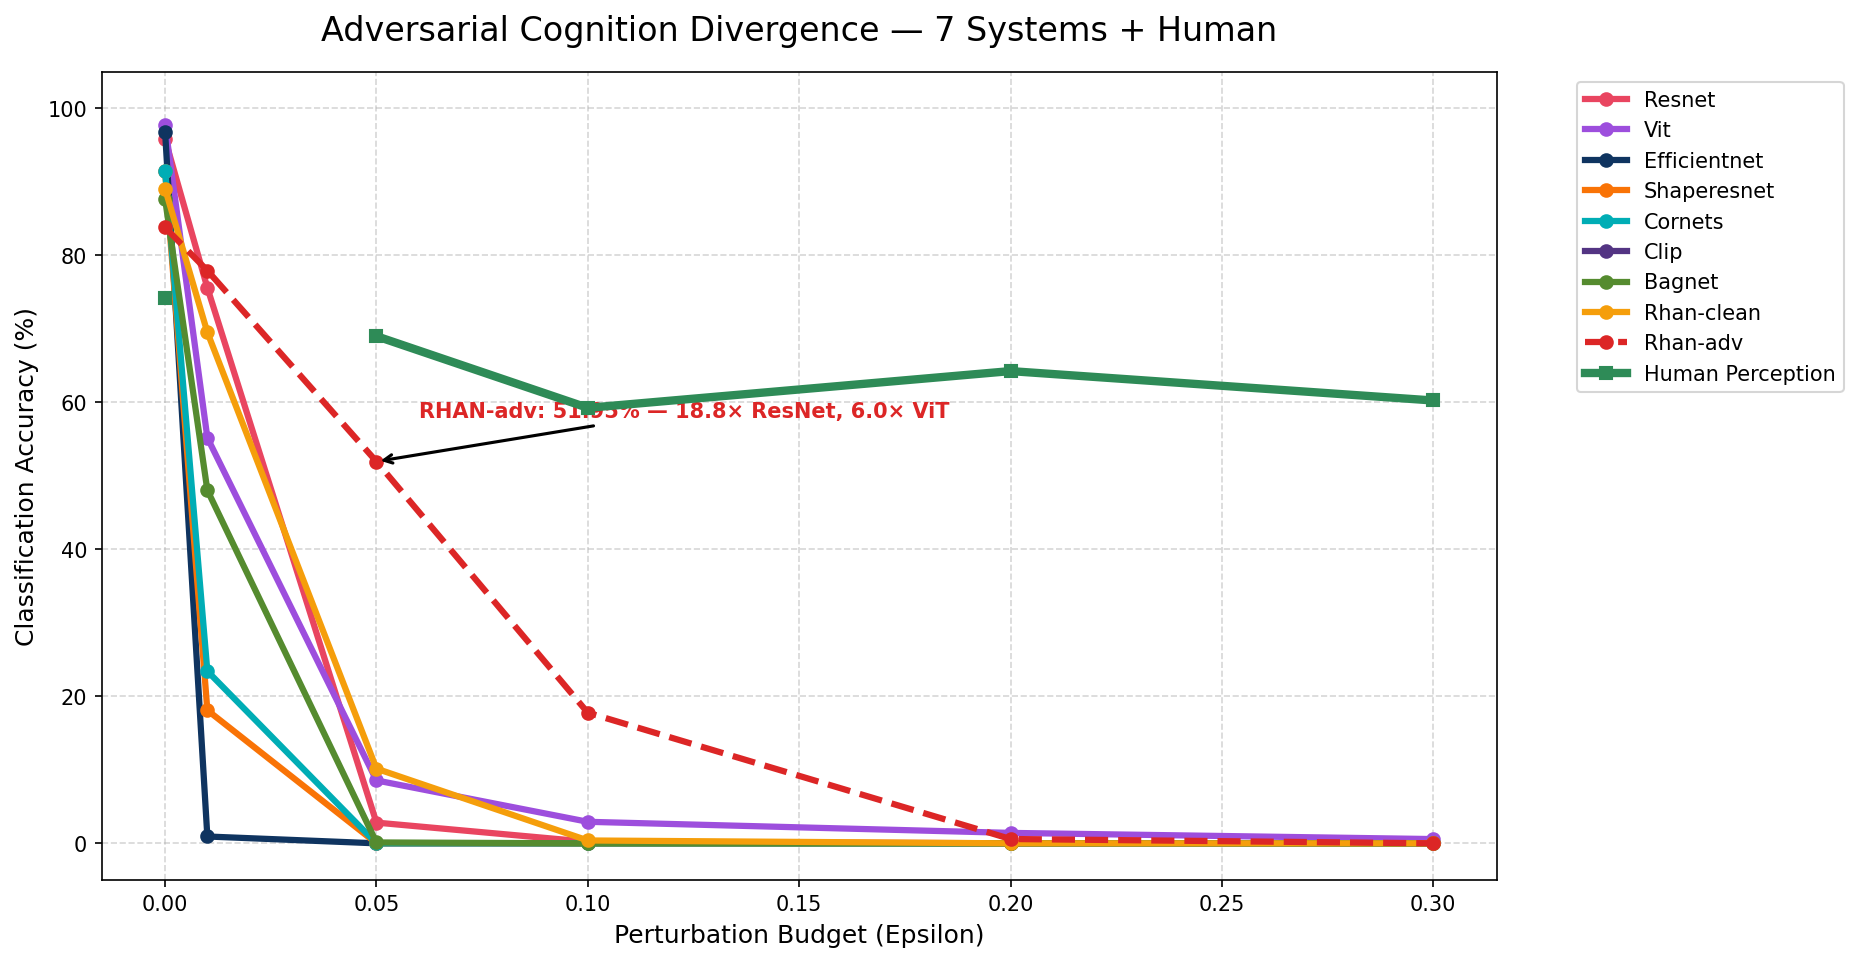
\includegraphics[width=\textwidth]{figures/FINAL_divergence_with_rhan.png}
  \caption{Accuracy divergence curves (Fig.~A.1).}
  \label{fig:div_acc_full}
\end{subfigure}
\hfill
\begin{subfigure}[b]{0.48\textwidth}
  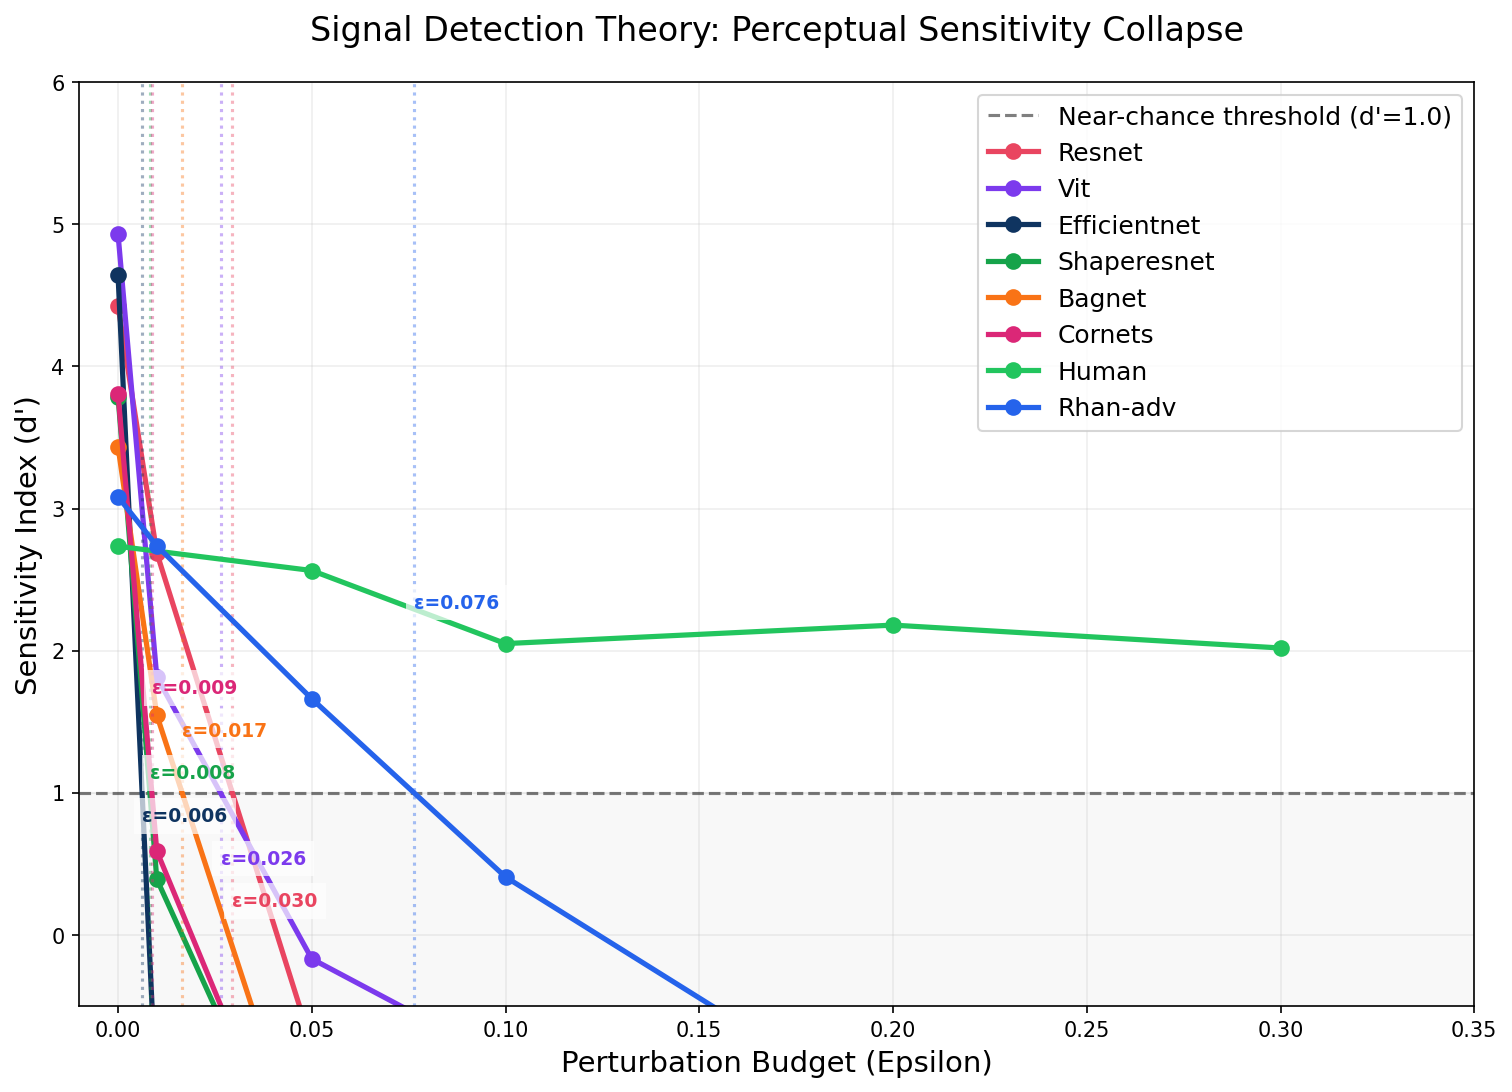
\includegraphics[width=\textwidth]{figures/final_dprime_with_rhan.png}
  \caption{SDT $d'$ sensitivity curves (Fig.~A.2).}
  \label{fig:div_dprime_full}
\end{subfigure}
\caption{\textbf{Unified Accuracy and Perceptual Sensitivity Curves}
across twelve architectures and human vision.}
\label{fig:unified_curves_full}
\end{figure}

\begin{figure}[H]
\centering
\begin{subfigure}[b]{0.48\textwidth}
  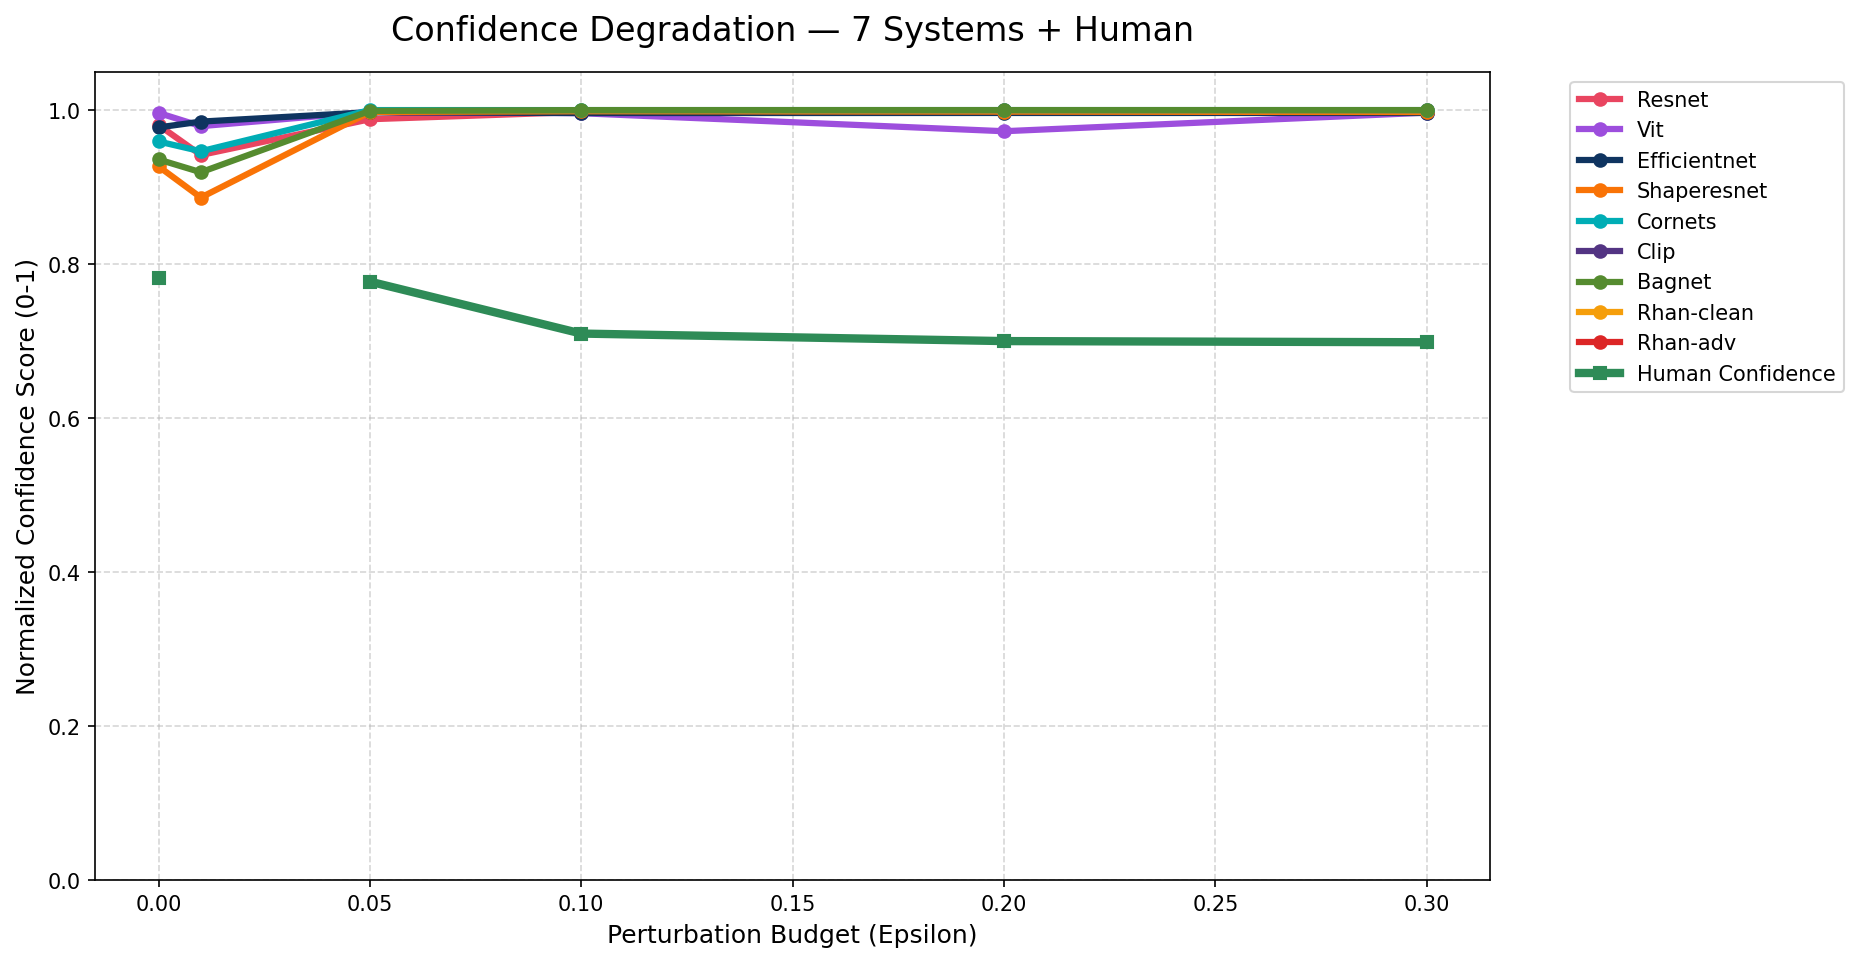
\includegraphics[width=\textwidth]{figures/full_confidence_curve.png}
  \caption{Confidence decay curves (Fig.~A.3).}
  \label{fig:confidence_decay_full}
\end{subfigure}
\hfill
\begin{subfigure}[b]{0.48\textwidth}
  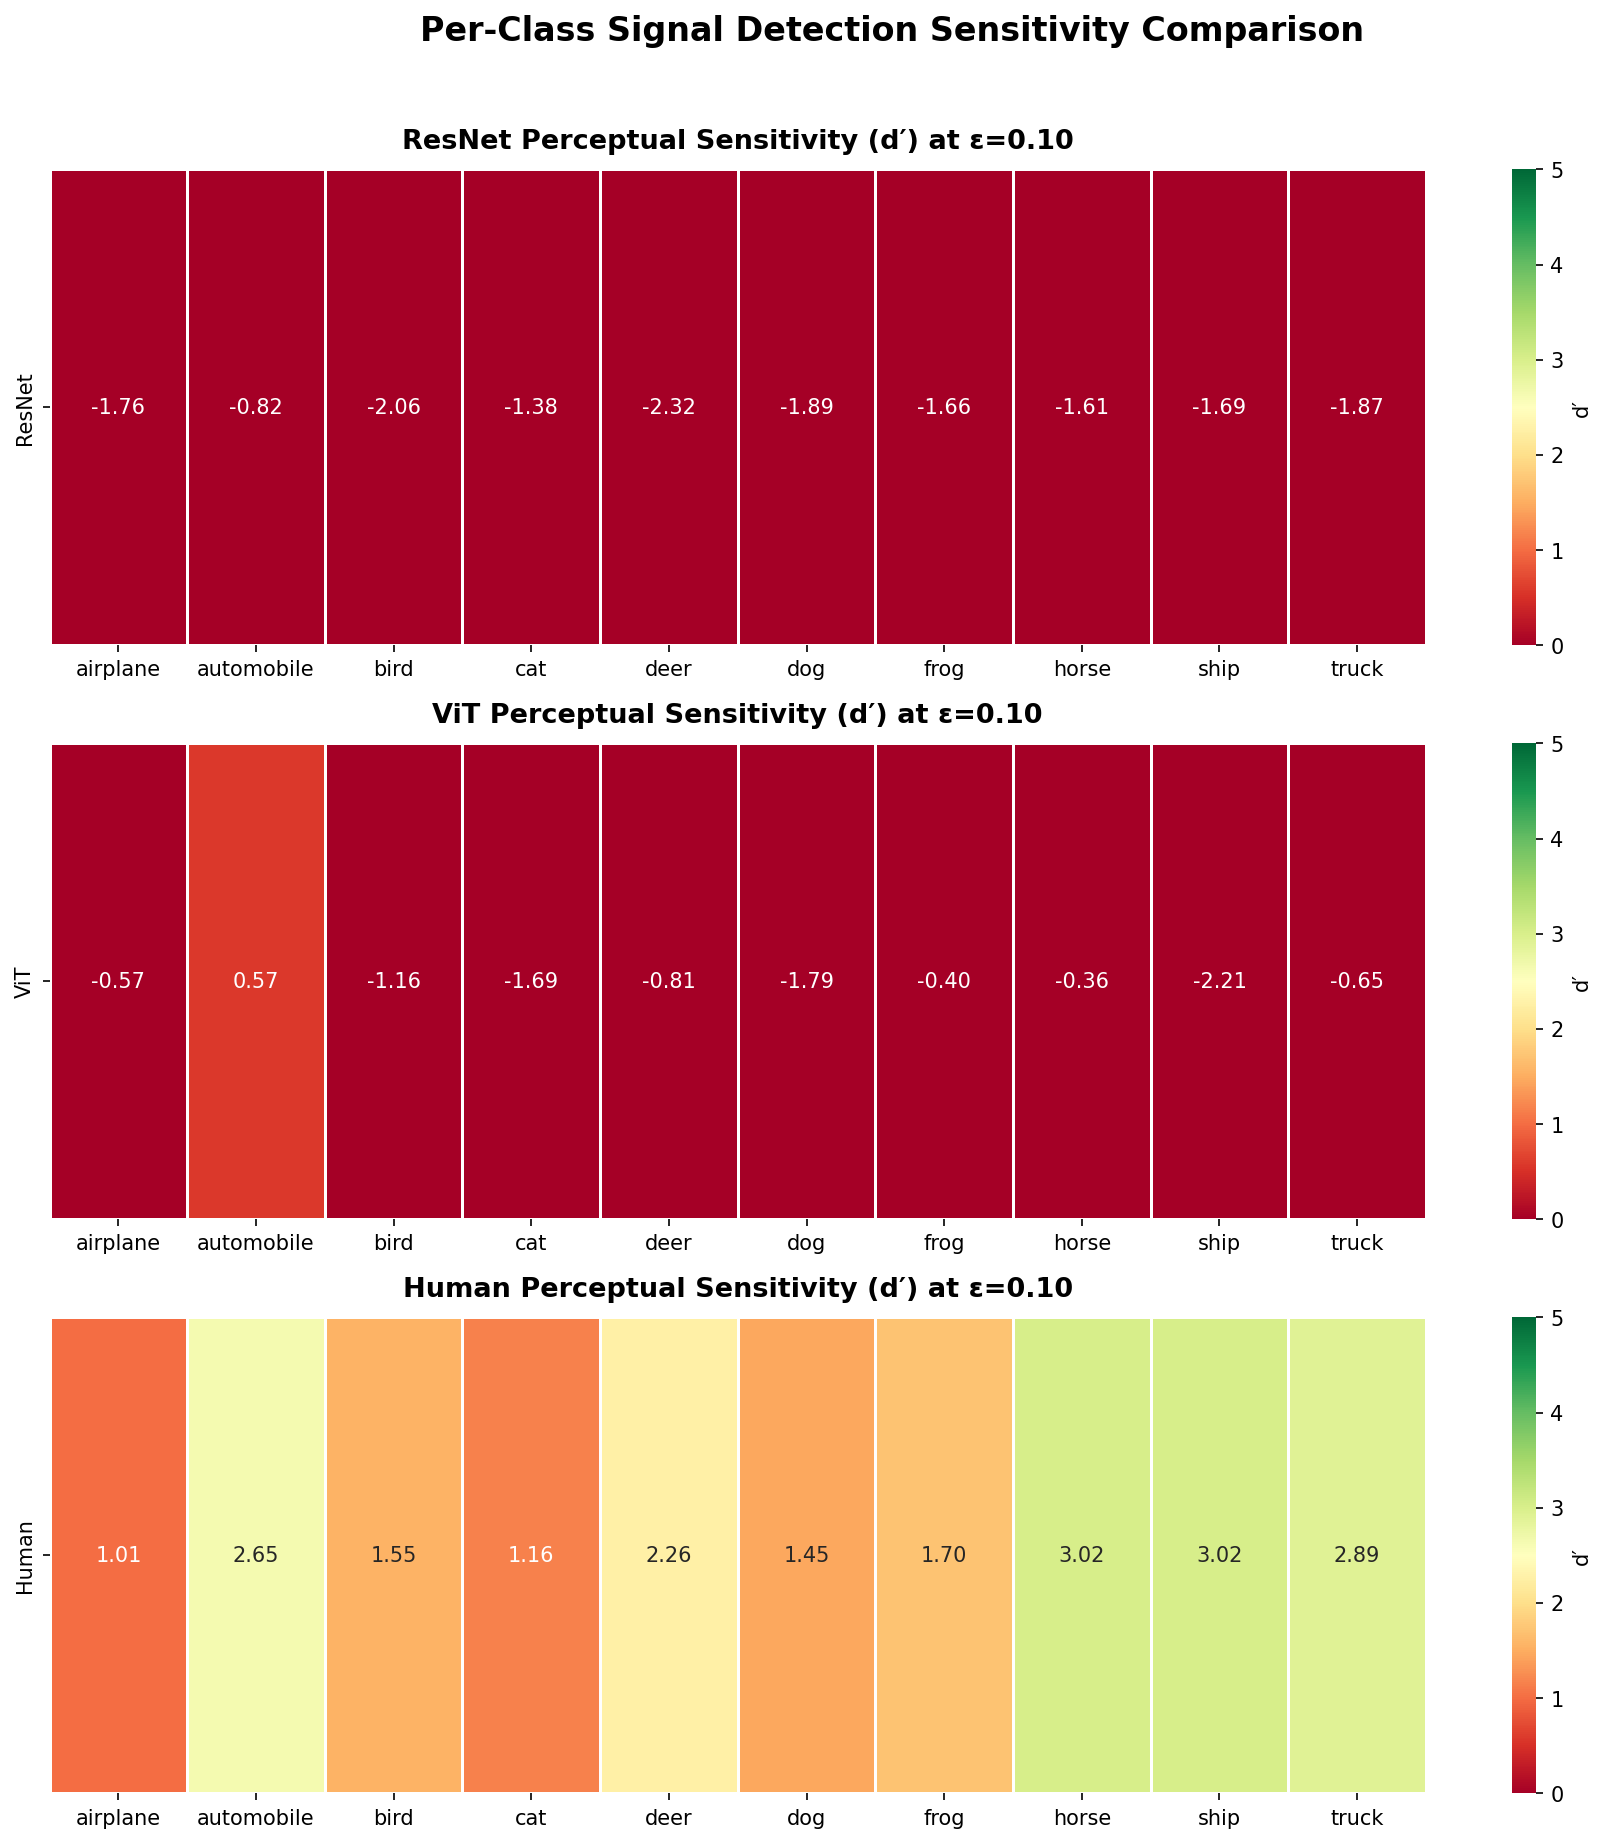
\includegraphics[width=\textwidth]{figures/perclass_dprime_eps0.10.png}
  \caption{Per-class $d'$ at $\varepsilon{=}0.10$ (Fig.~A.4).}
  \label{fig:perclass_dprime_full}
\end{subfigure}
\caption{\textbf{Confidence Calibration and Semantic Class Sensitivity}.}
\label{fig:confidence_and_perclass_full}
\end{figure}

\begin{figure}[H]
\centering
\begin{subfigure}[b]{0.48\textwidth}
  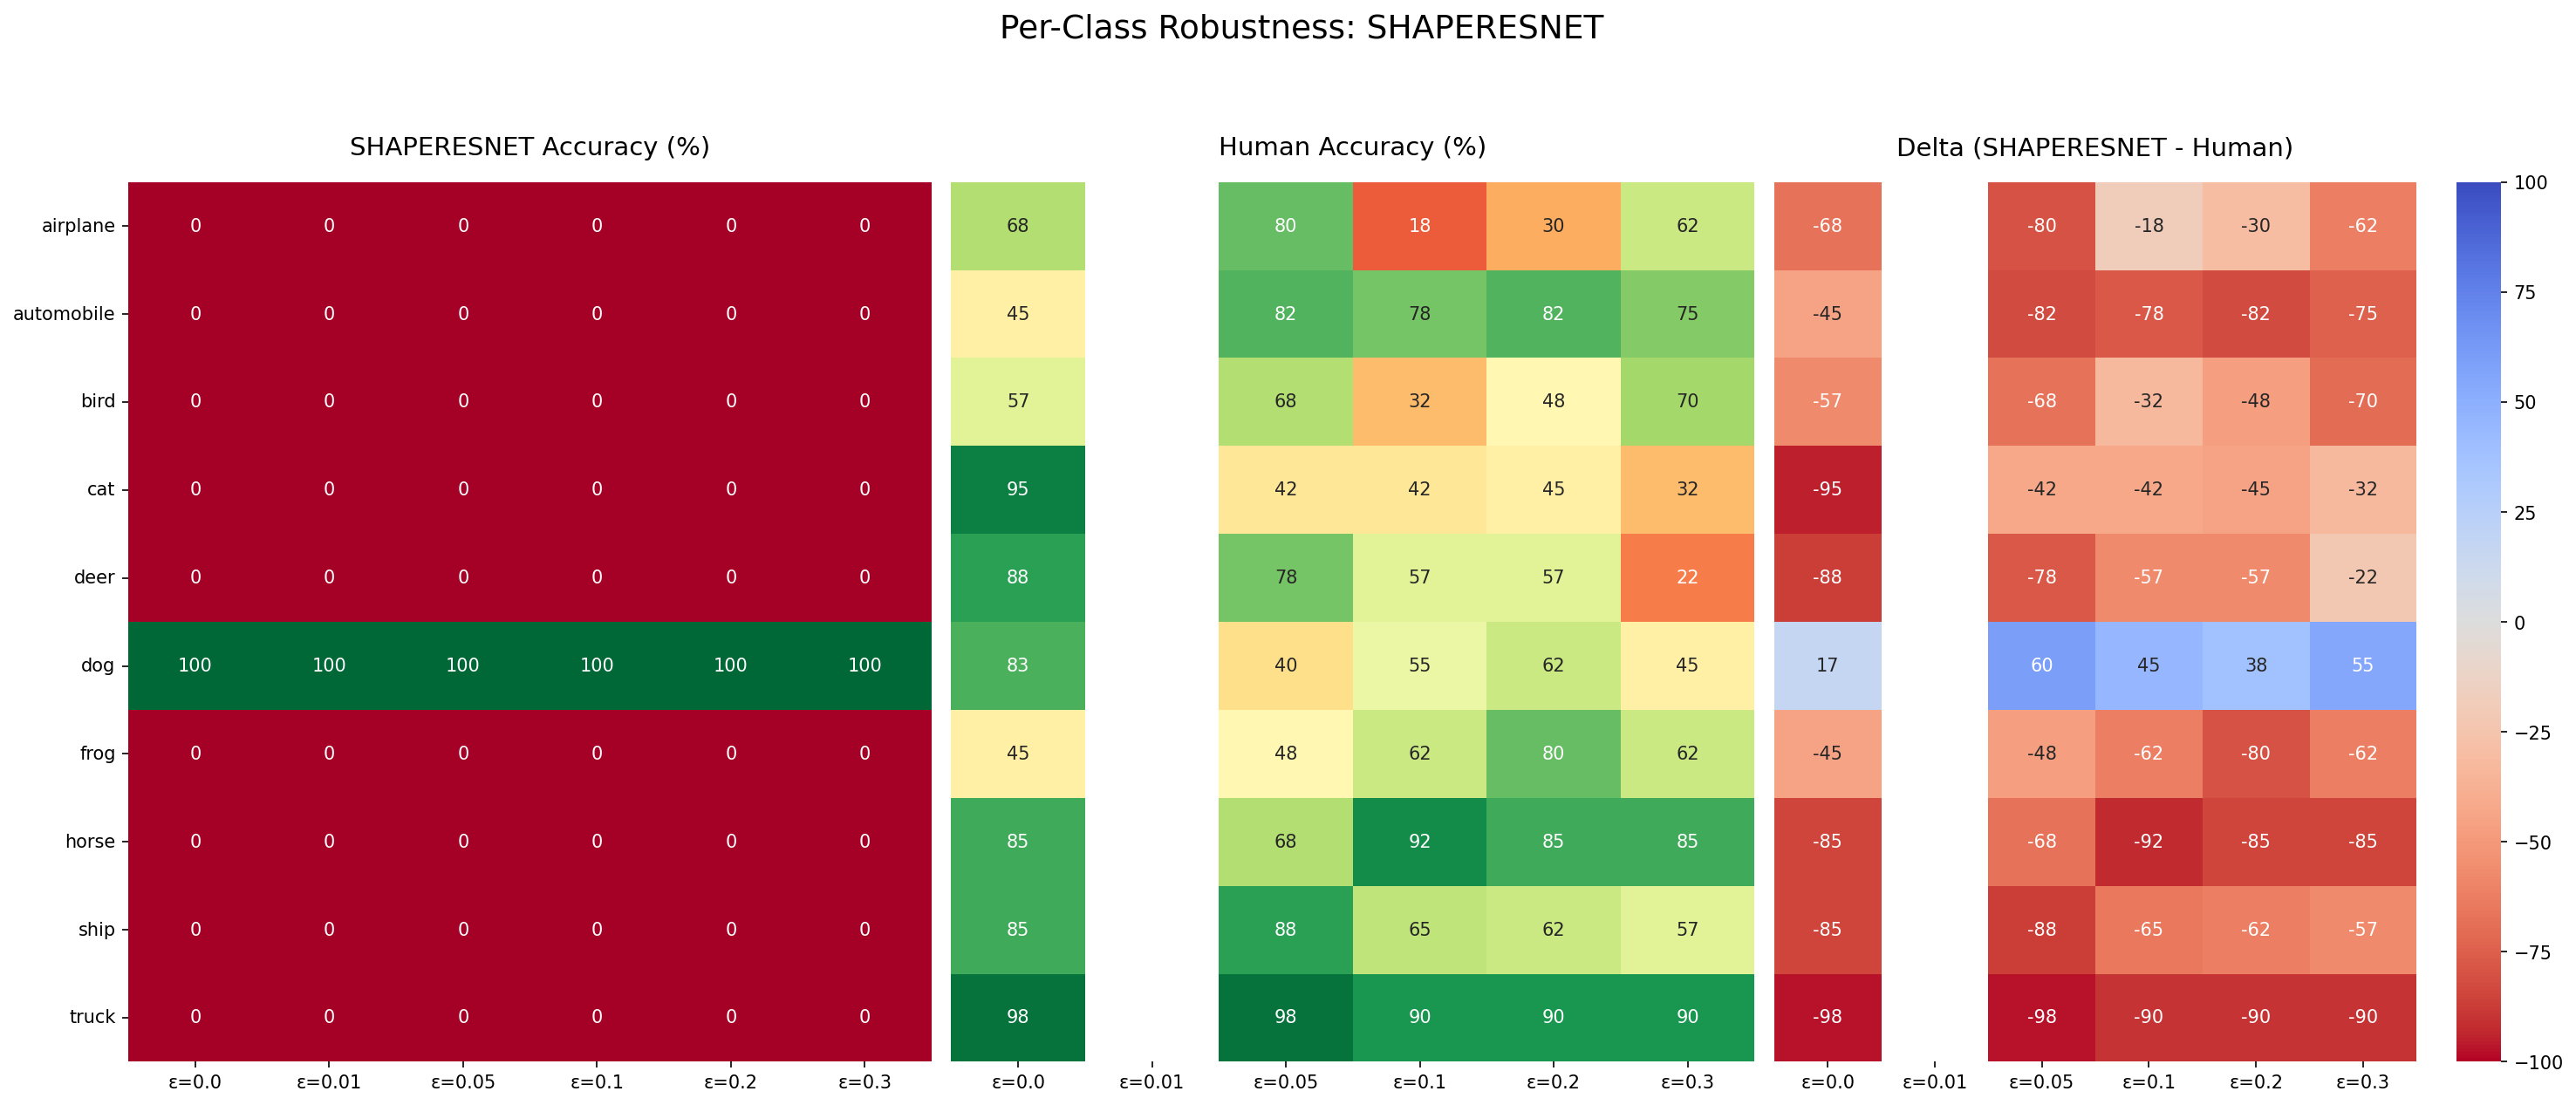
\includegraphics[width=\textwidth]{figures/class_heatmap.png}
  \caption{Machine Performance Accuracy Heatmap (Fig.~A.5).}
  \label{fig:machine_heatmap}
\end{subfigure}
\hfill
\begin{subfigure}[b]{0.48\textwidth}
  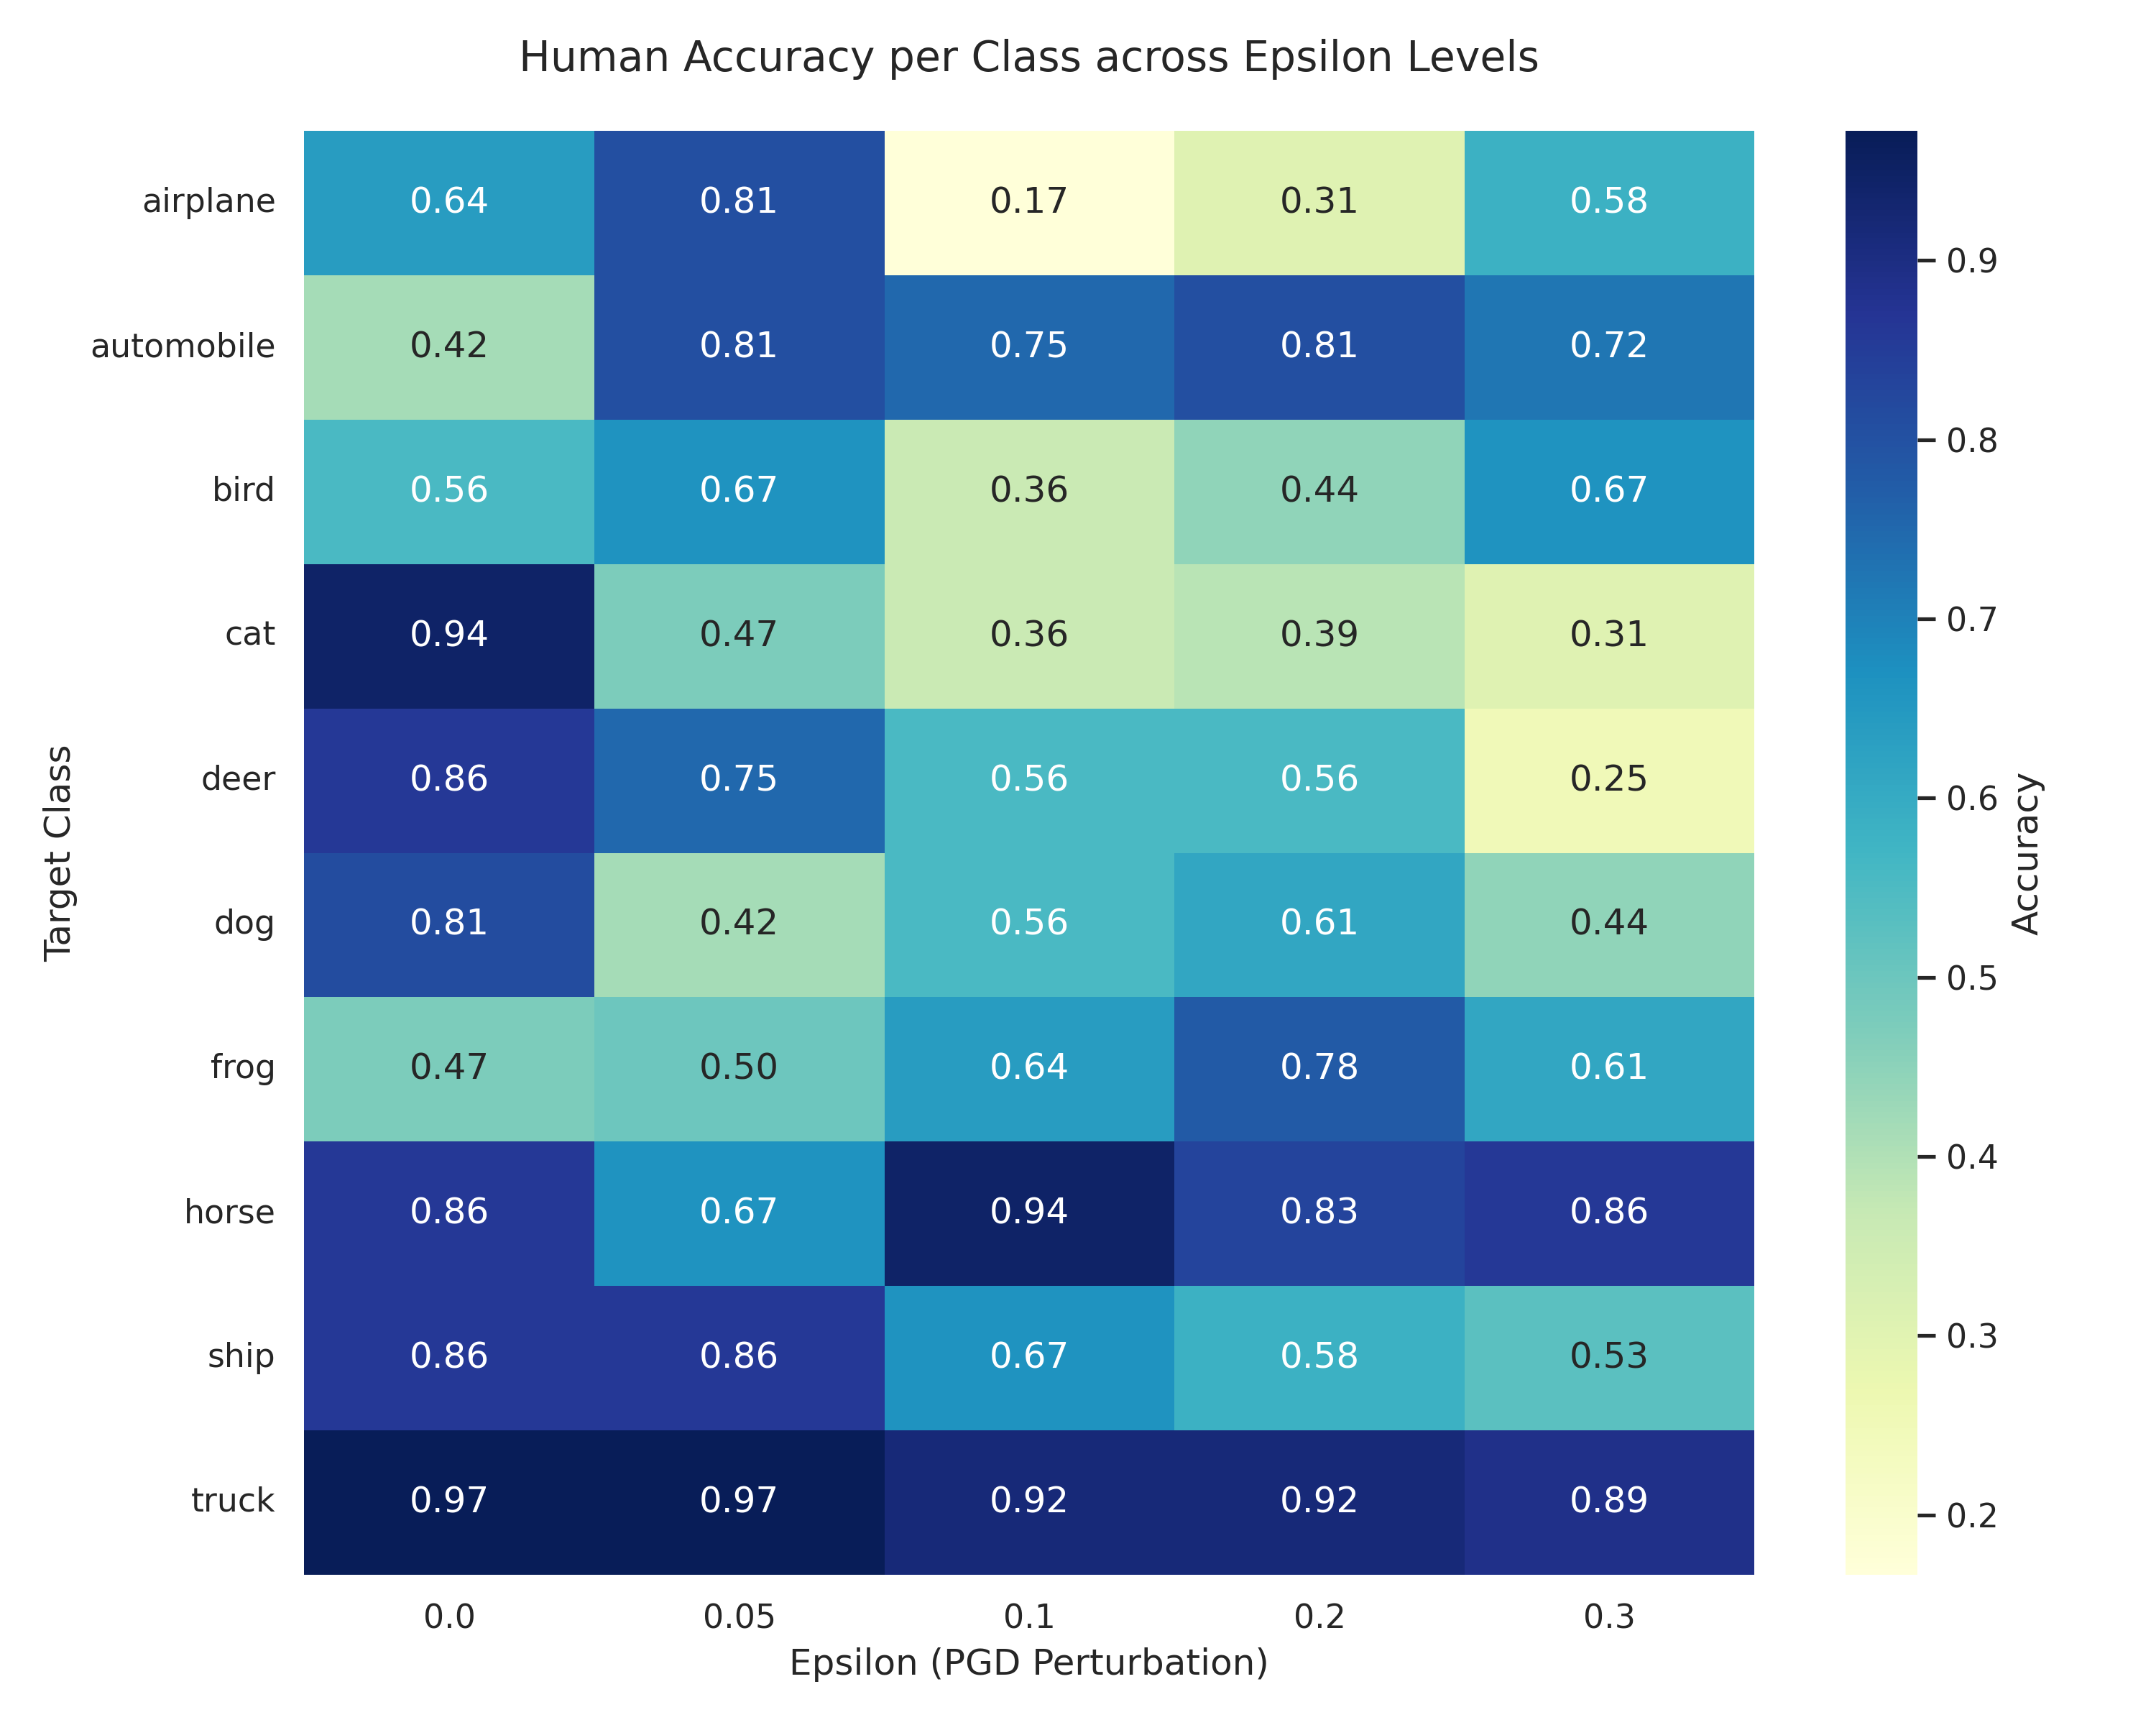
\includegraphics[width=\textwidth]{figures/human_class_heatmap.png}
  \caption{Human Performance Accuracy Heatmap (Fig.~A.6).}
  \label{fig:human_heatmap}
\end{subfigure}
\caption{\textbf{Semantic Class Accuracy Heatmaps across Epsilon Budgets}.}
\label{fig:class_heatmaps}
\end{figure}

\begin{figure}[H]
\centering
\begin{subfigure}[b]{0.48\textwidth}
  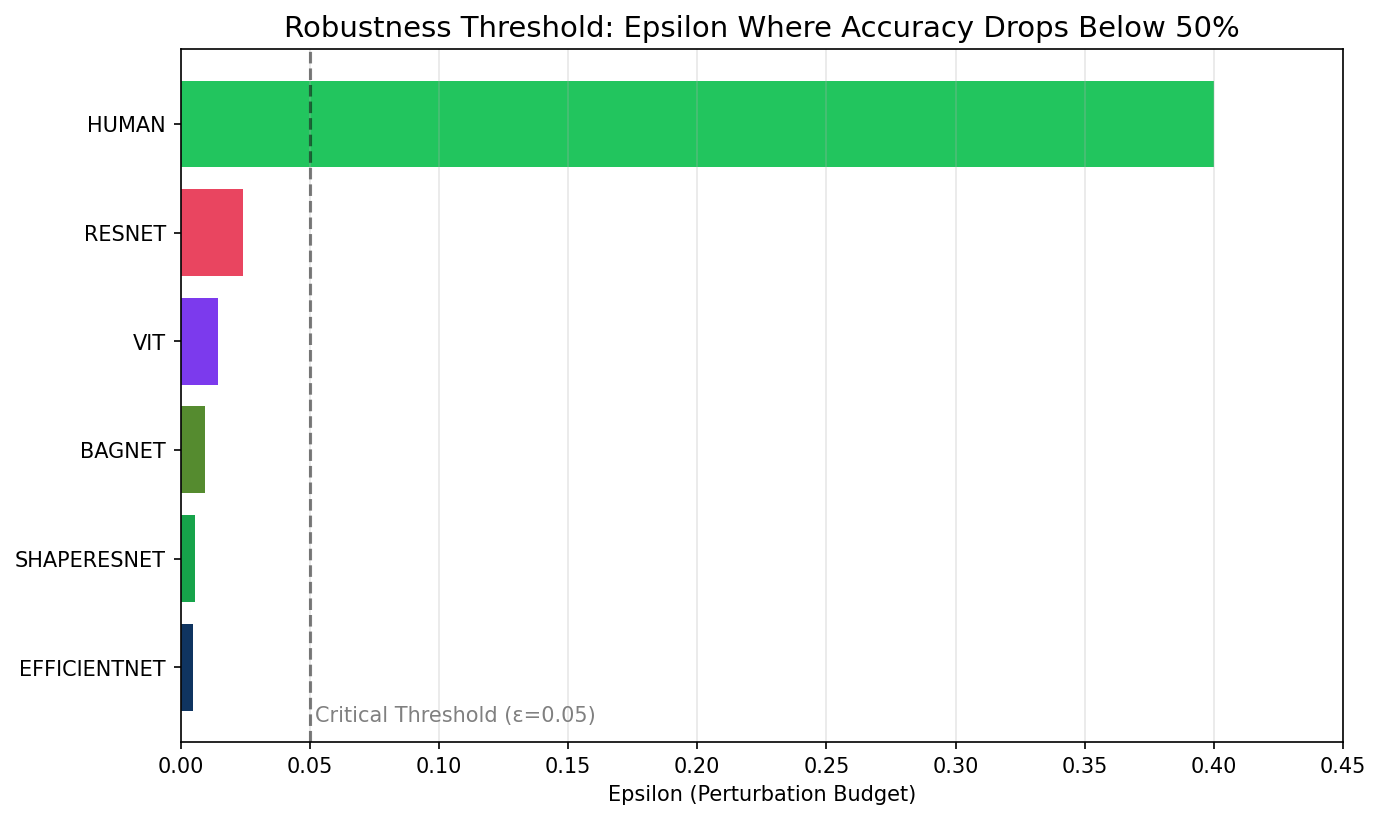
\includegraphics[width=\textwidth]{figures/accuracy_threshold_bars.png}
  \caption{Accuracy-based Thresholds (Fig.~A.7).}
  \label{fig:acc_thresholds}
\end{subfigure}
\hfill
\begin{subfigure}[b]{0.48\textwidth}
  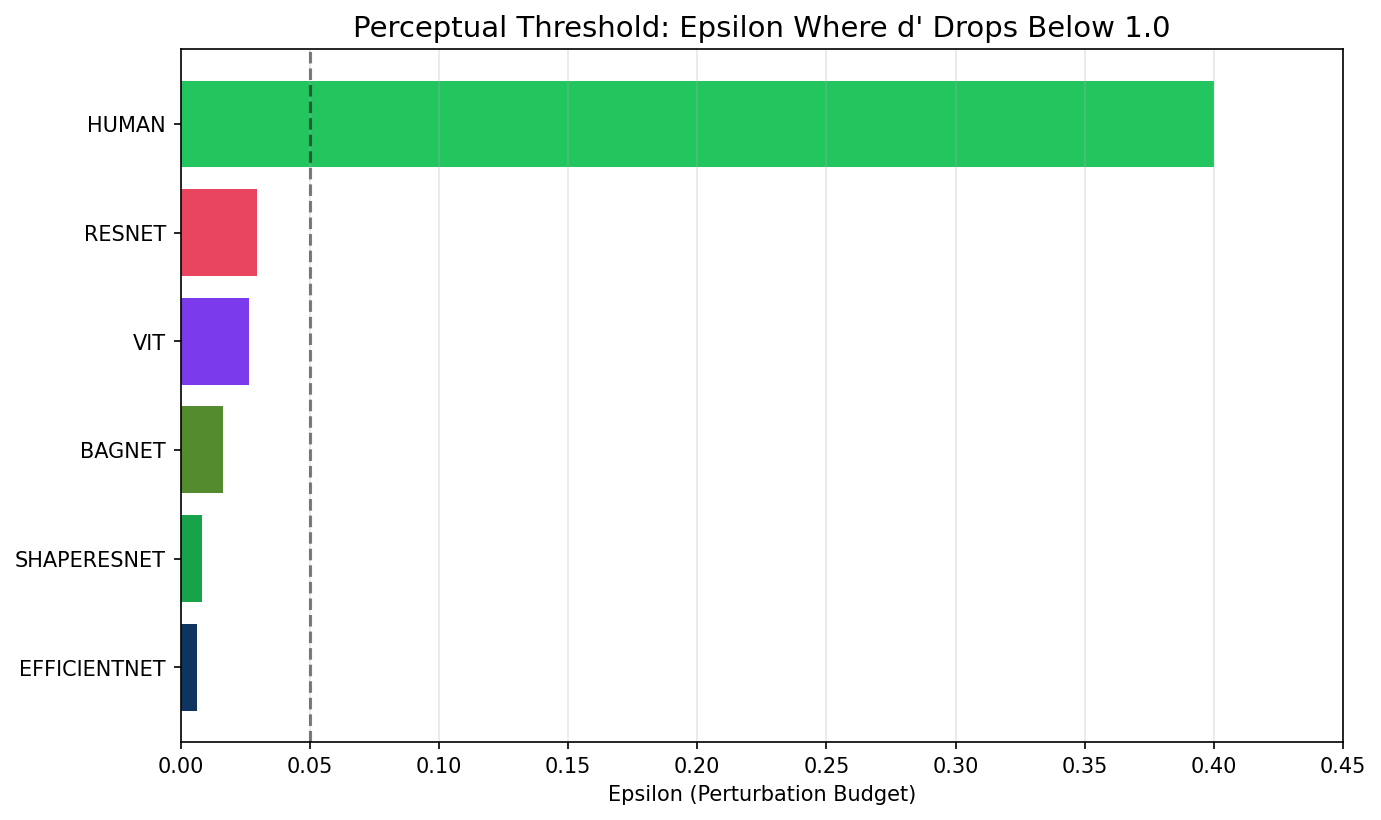
\includegraphics[width=\textwidth]{figures/sdt_threshold_bars.png}
  \caption{SDT Sensitivity Thresholds (Fig.~A.8).}
  \label{fig:sdt_thresholds}
\end{subfigure}
\caption{\textbf{Empirical and Perceptual Robustness Thresholds}.}
\label{fig:threshold_bars}
\end{figure}


% ============================================================
\section{Representation and Latent Space Topology}
\label{app:latent}
% ============================================================

\begin{figure}[H]
\centering
\begin{subfigure}[b]{0.48\textwidth}
  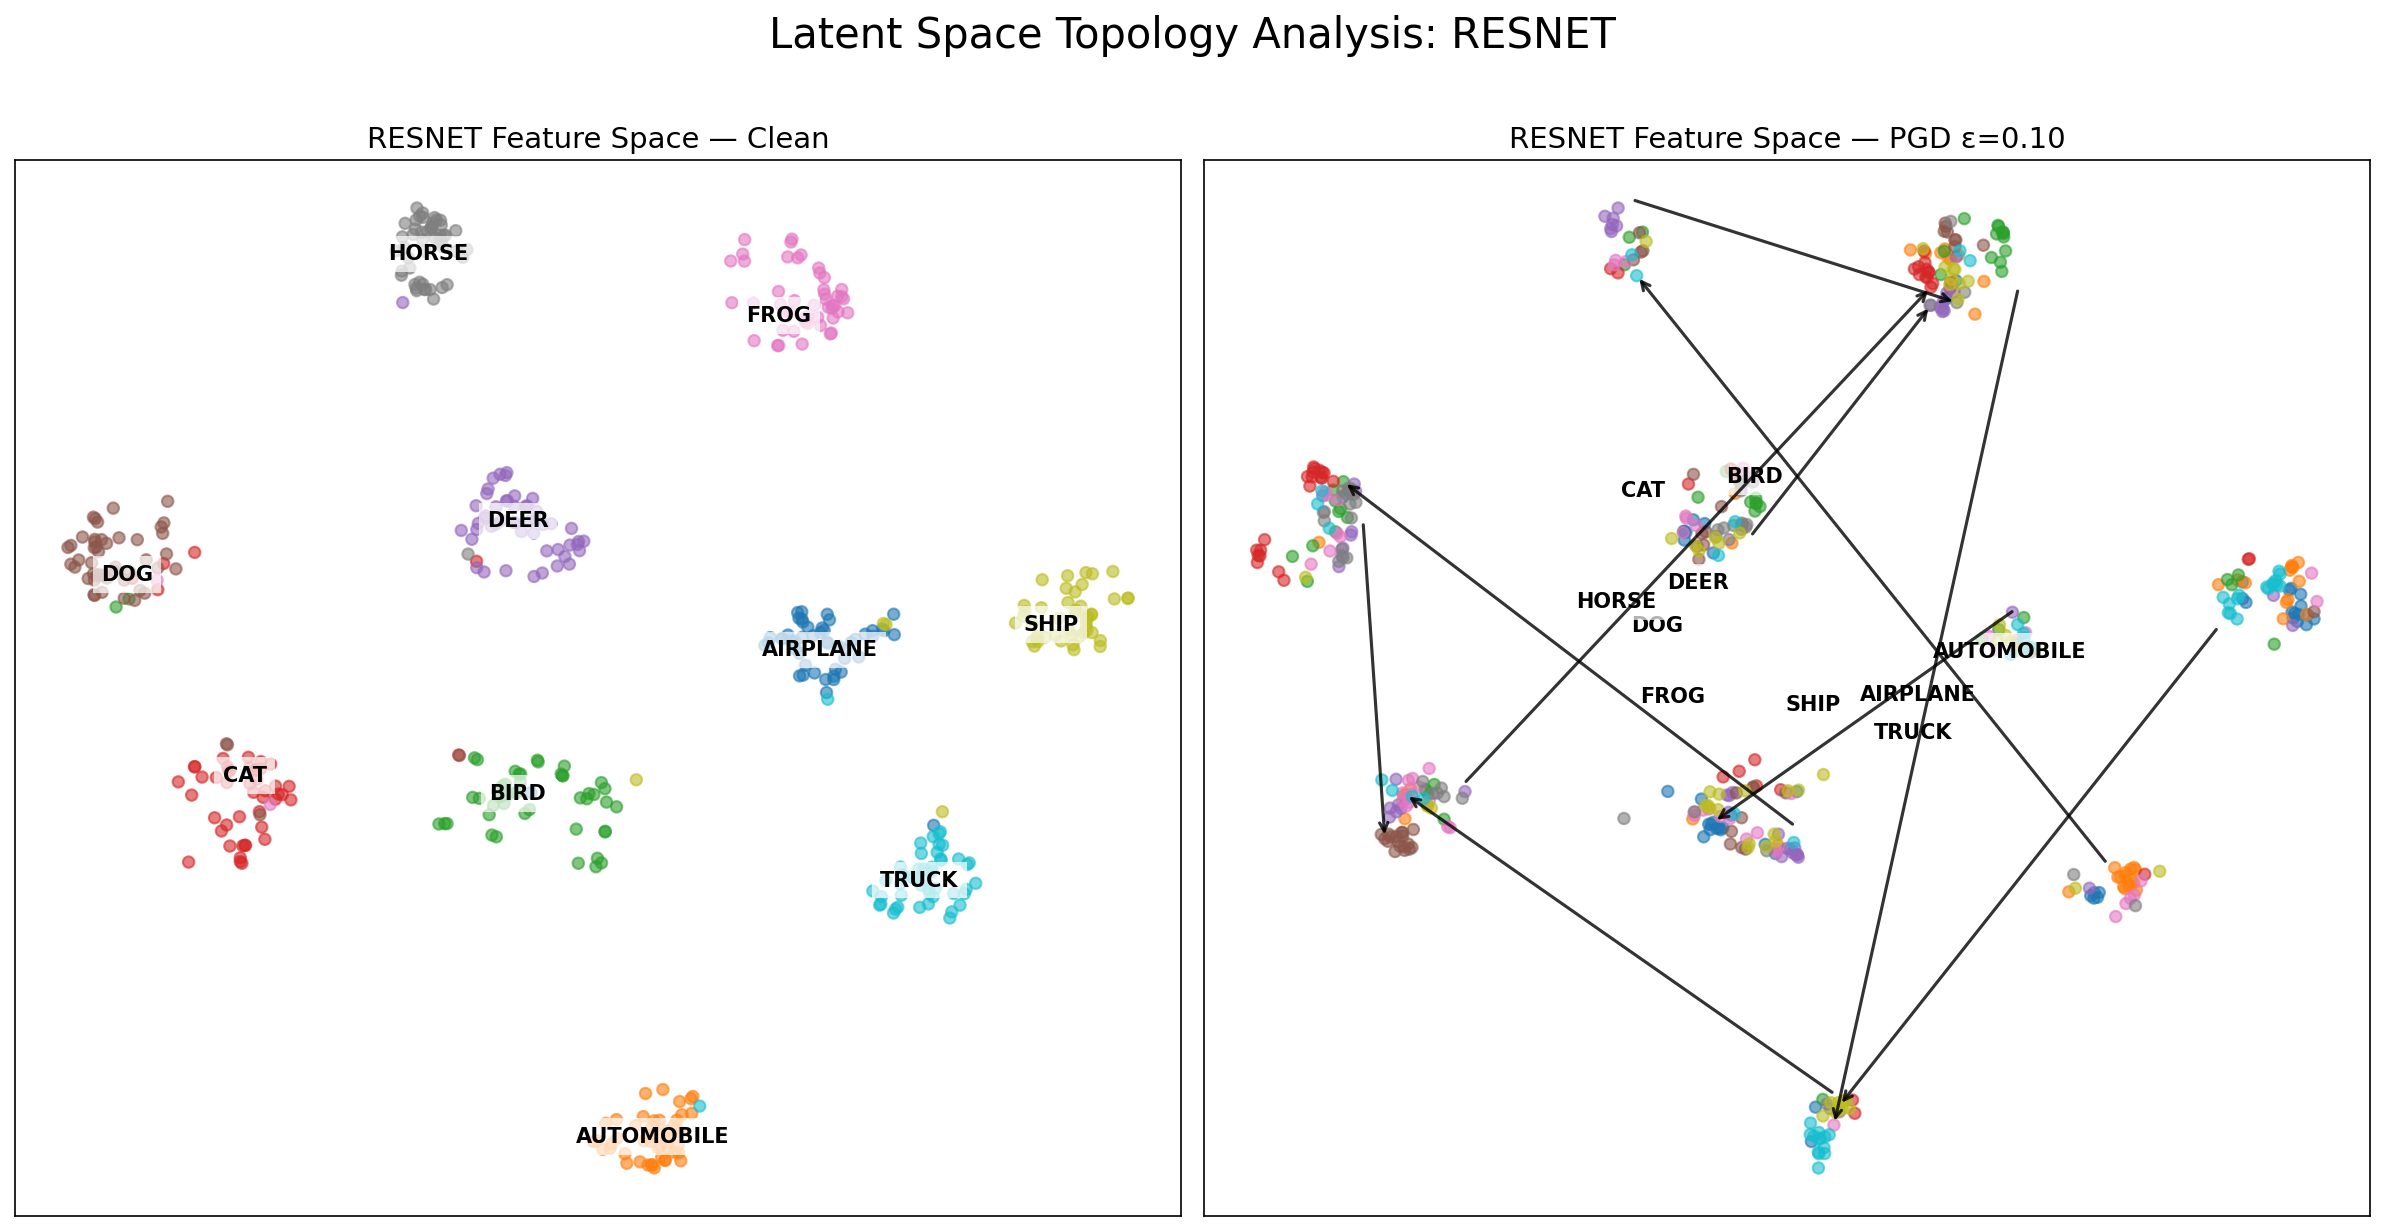
\includegraphics[width=\textwidth]{figures/resnet_tsne.png}
  \caption{ResNet-18 latent t-SNE (Fig.~A.9).}
\end{subfigure}
\hfill
\begin{subfigure}[b]{0.48\textwidth}
  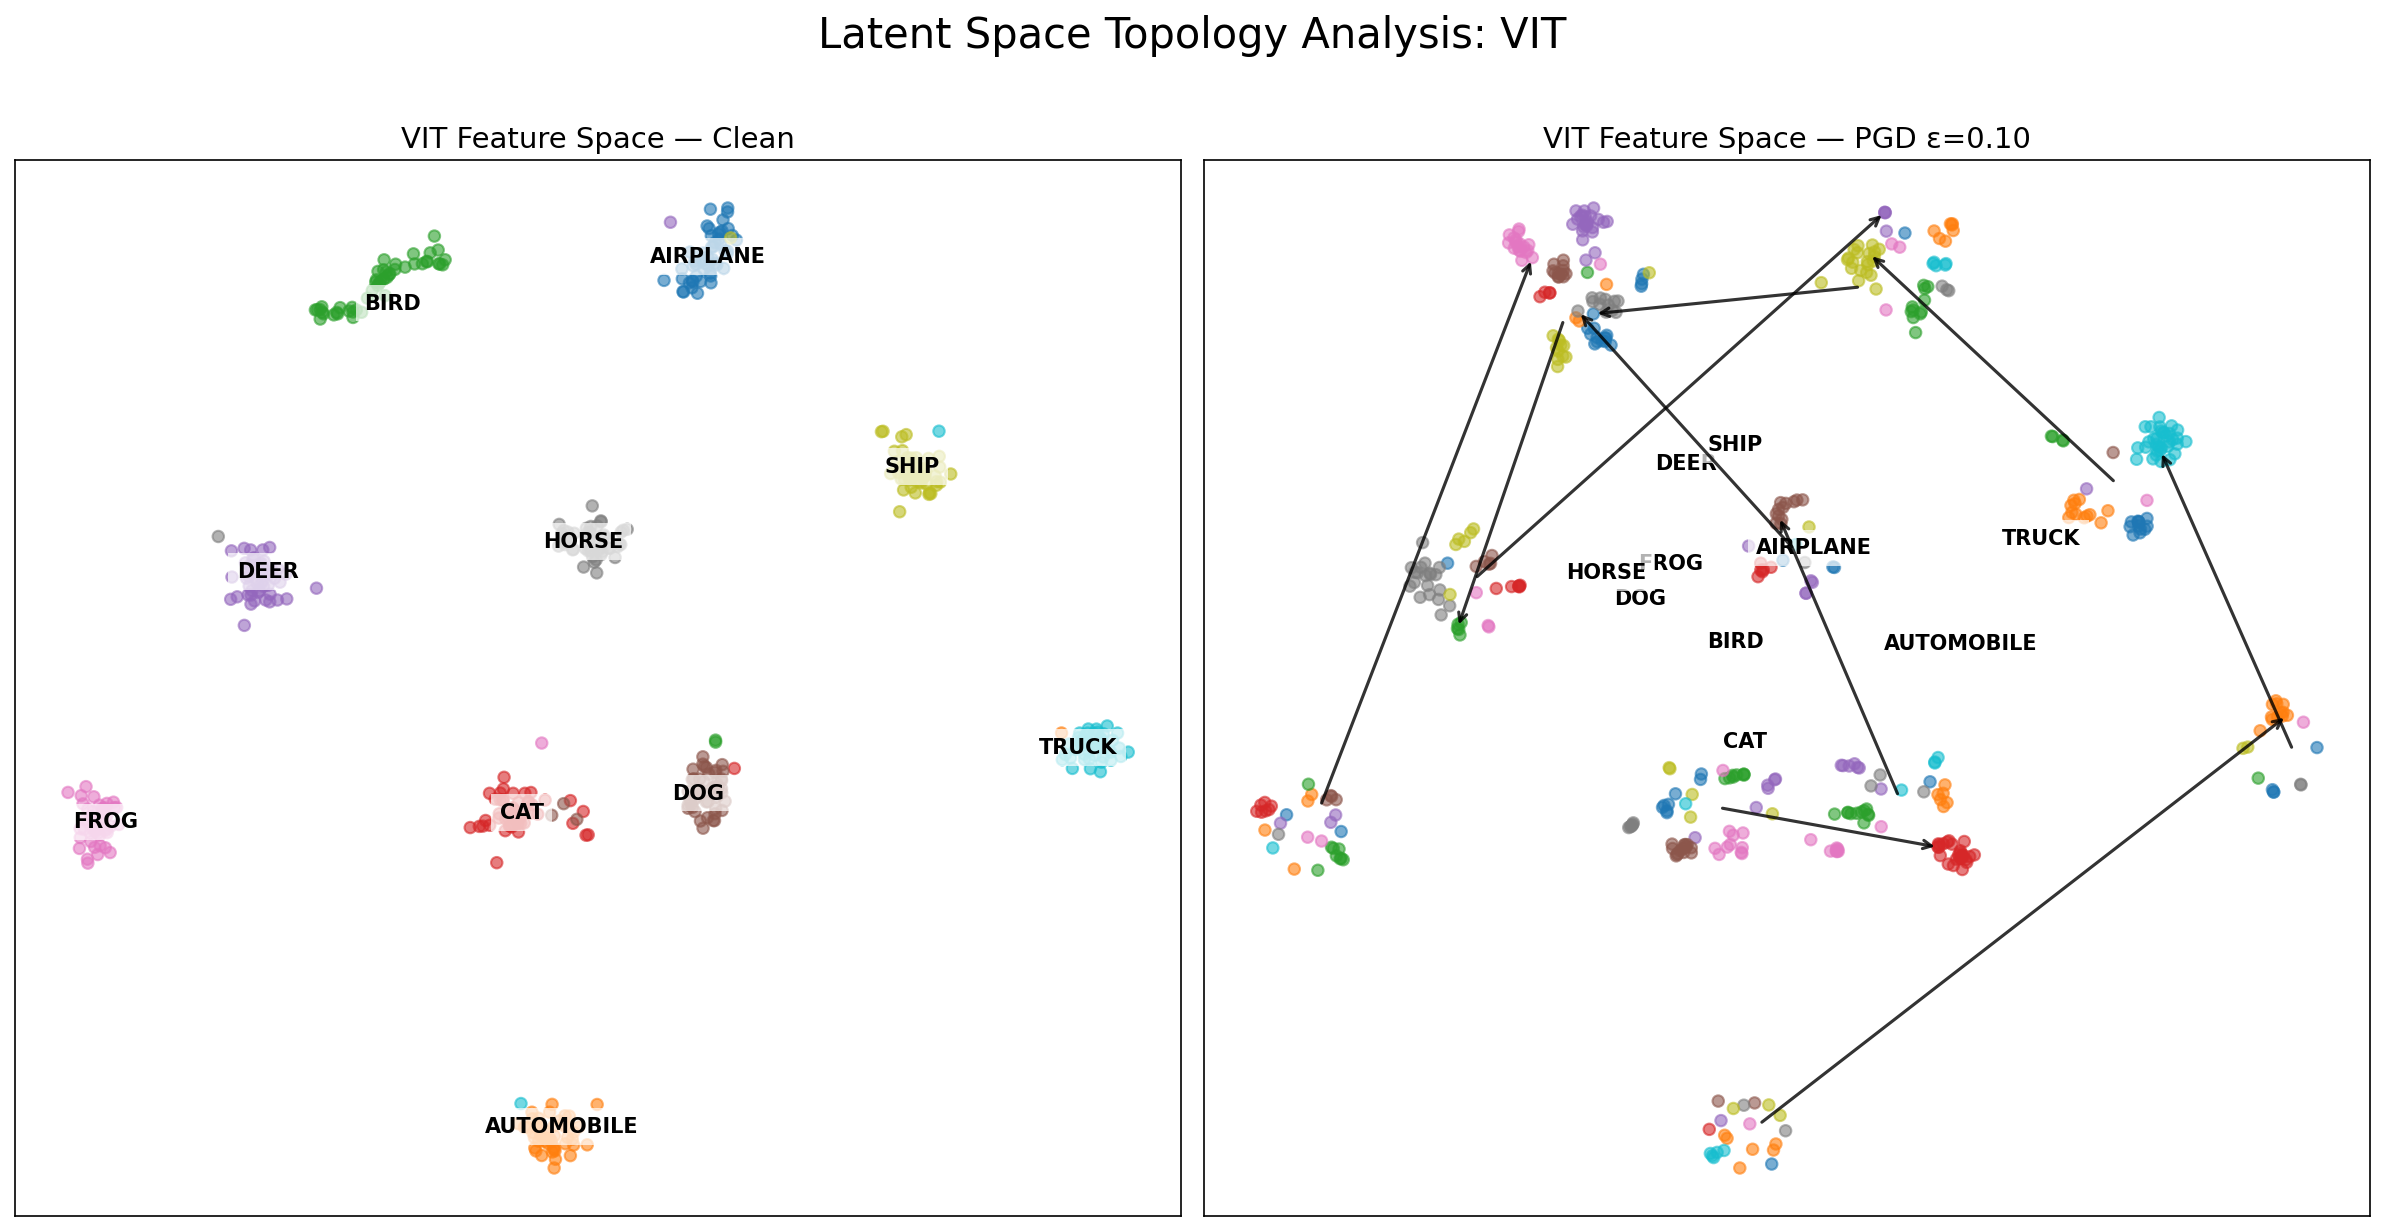
\includegraphics[width=\textwidth]{figures/vit_tsne.png}
  \caption{ViT-Small latent t-SNE (Fig.~A.10).}
\end{subfigure}
\caption{\textbf{Latent Feature Space Displacement t-SNE Projections}.}
\end{figure}

\begin{figure}[H]
\centering
\begin{subfigure}[b]{0.48\textwidth}
  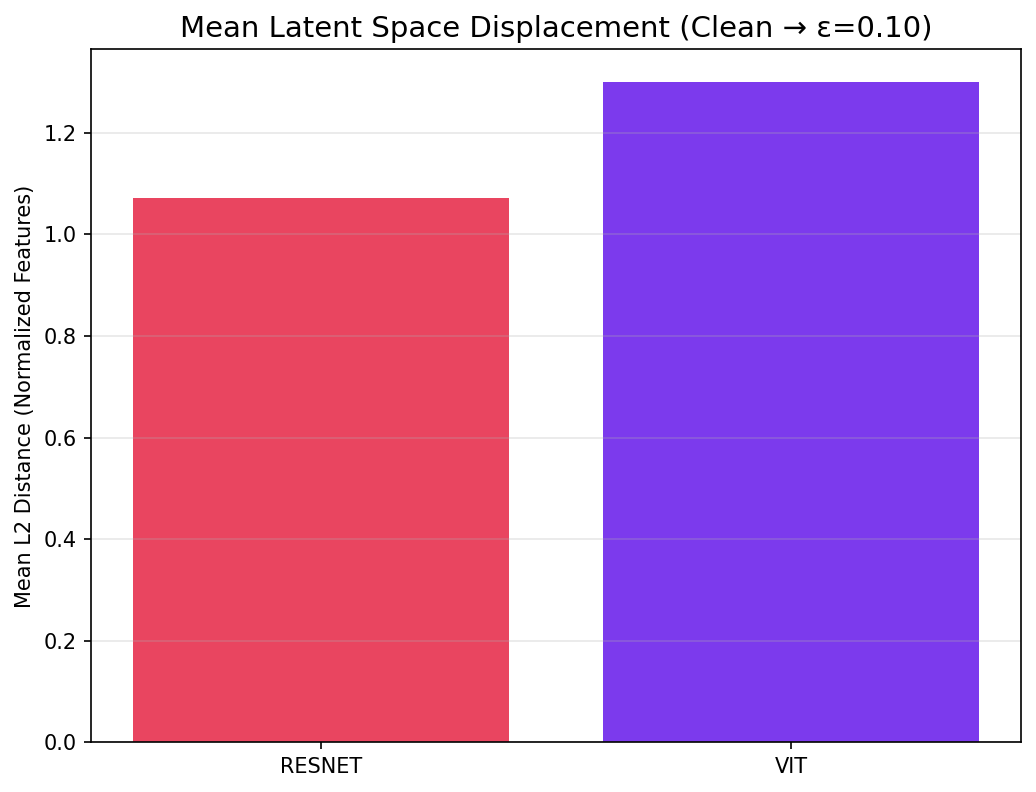
\includegraphics[width=\textwidth]{figures/displacement_comparison.bar.png}
  \caption{Latent space centroid displacement (Fig.~A.11).}
\end{subfigure}
\hfill
\begin{subfigure}[b]{0.48\textwidth}
  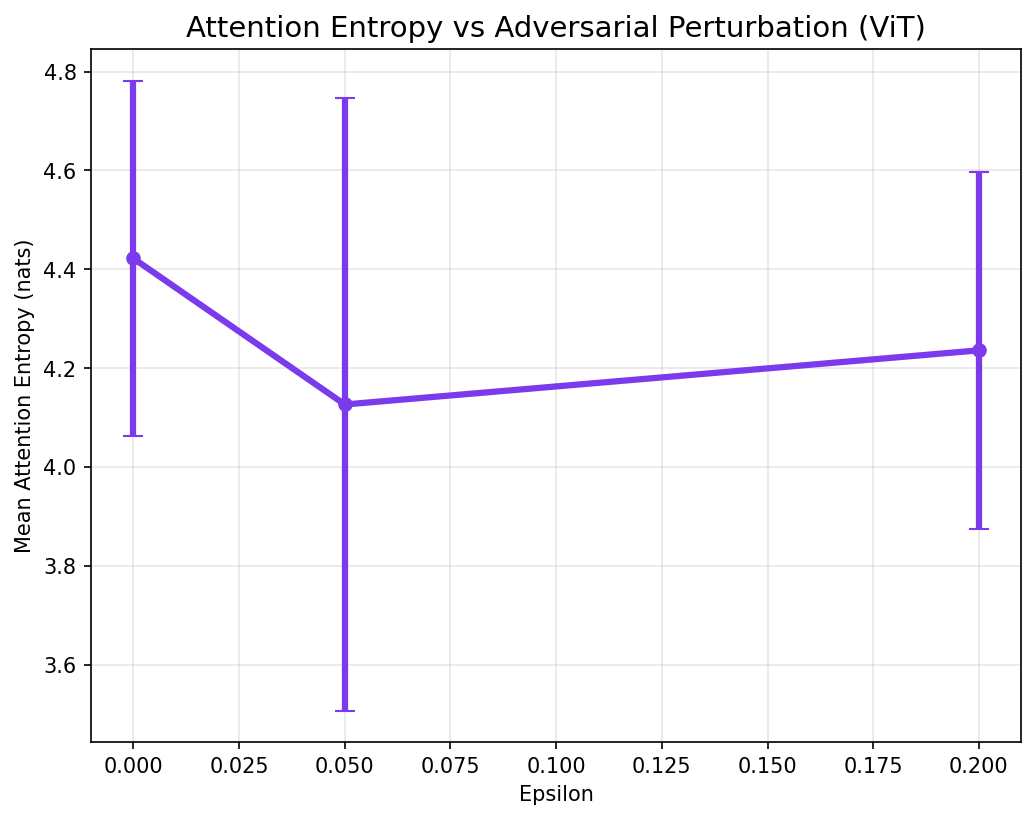
\includegraphics[width=\textwidth]{figures/vit_attention_entropy.png}
  \caption{ViT self-attention entropy decay (Fig.~A.12).}
\end{subfigure}
\caption{\textbf{Latent Displacement and Attention Entropy Analysis}.}
\end{figure}

\begin{figure}[H]
\centering
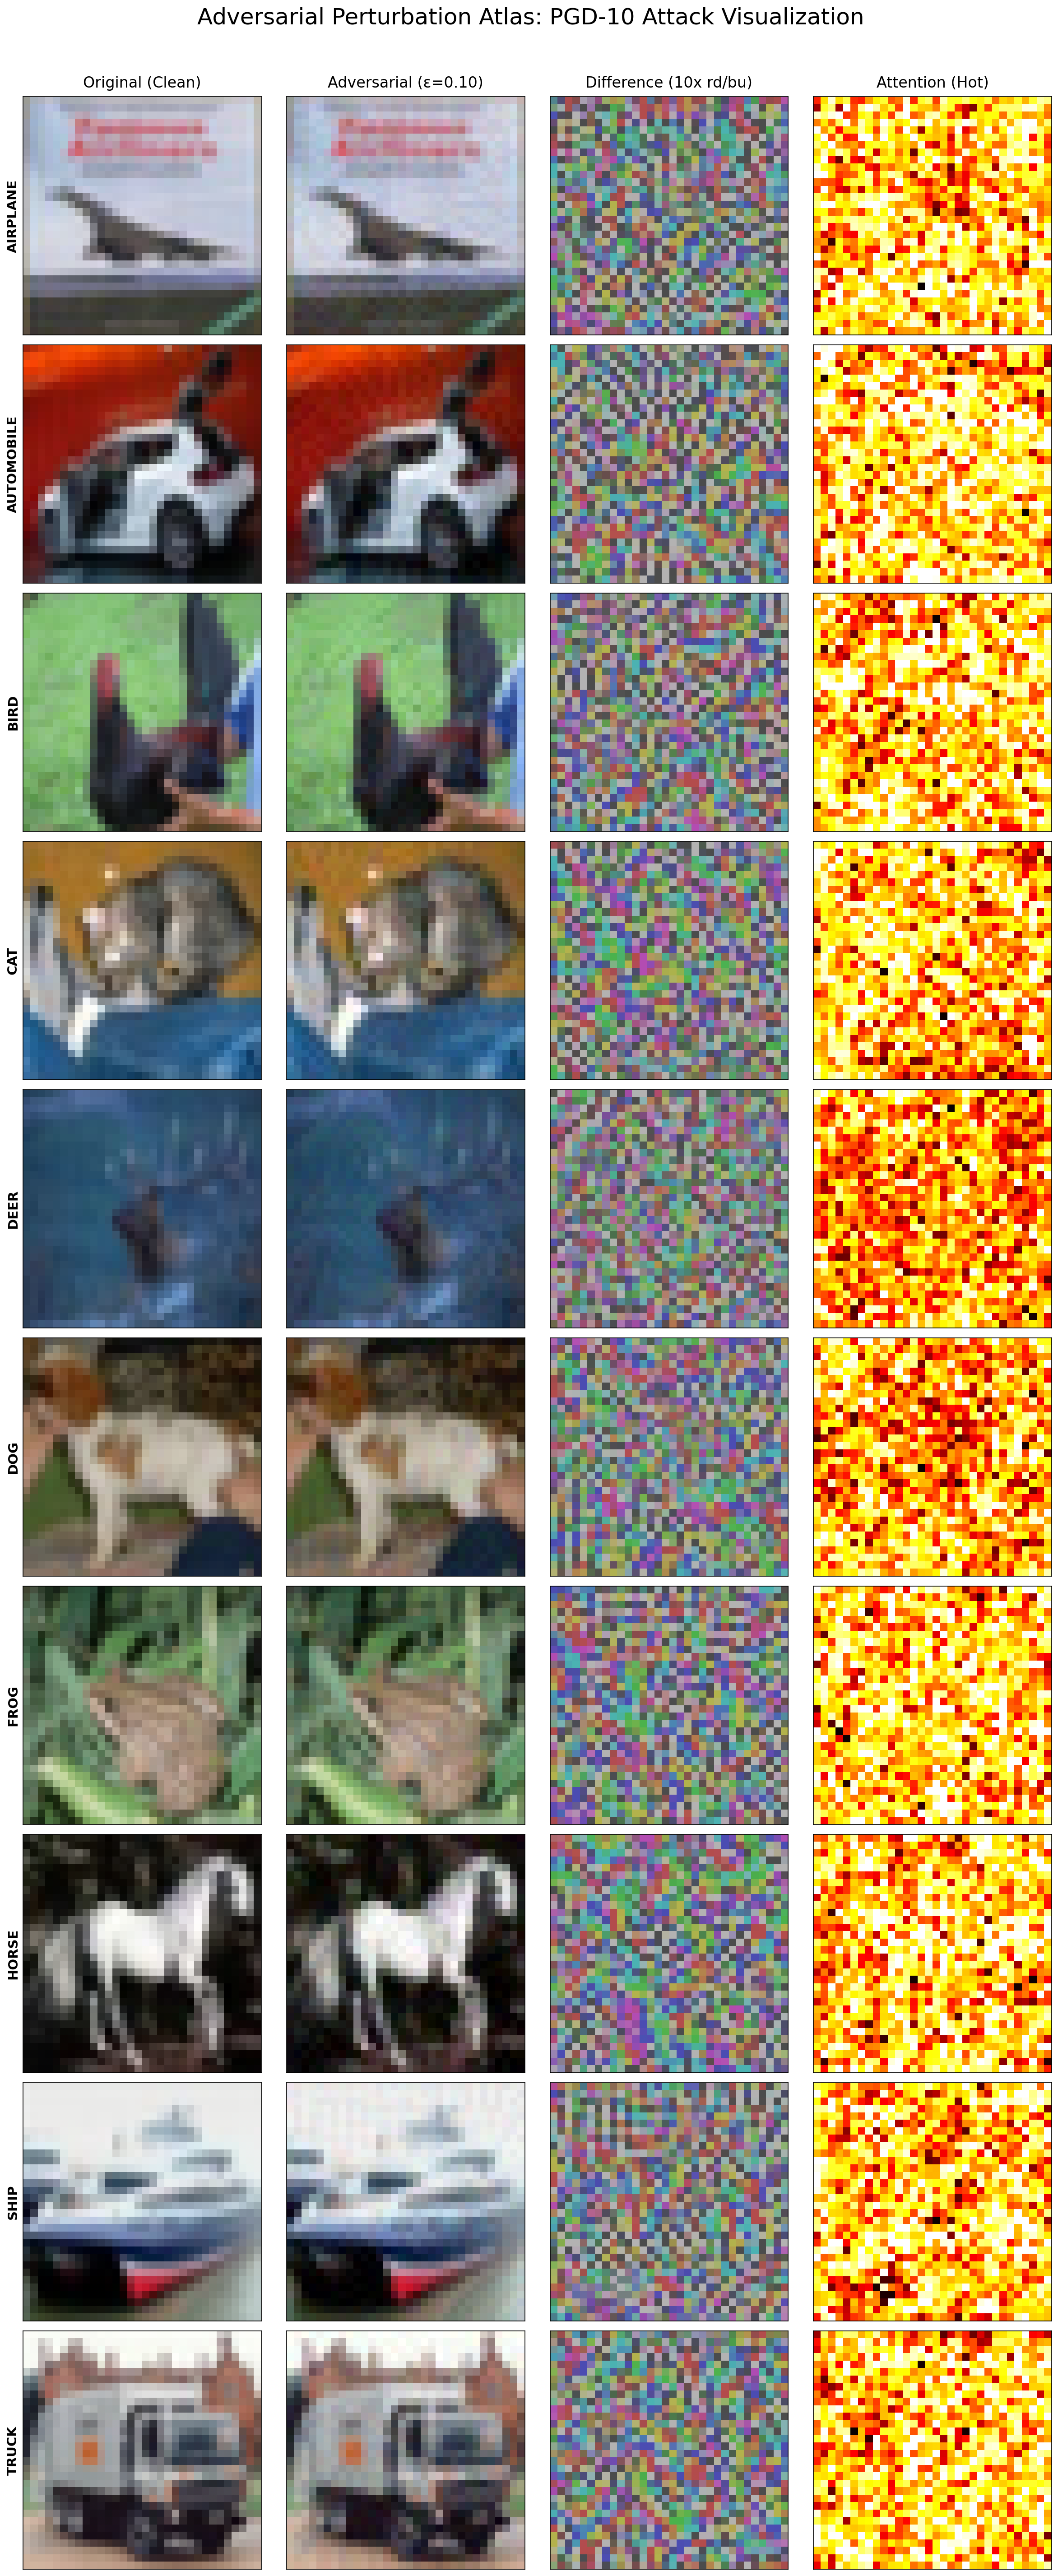
\includegraphics[width=0.9\textwidth]{figures/perturbation_atlas.png}
\caption{\textbf{The Adversarial Perturbation Atlas (Fig.~A.13)}.}
\end{figure}


% ============================================================
\section{Model-Specific Confusion Matrices}
\label{app:confusion}
% ============================================================

\begin{figure}[H]
\centering
\begin{subfigure}[b]{0.48\textwidth}
  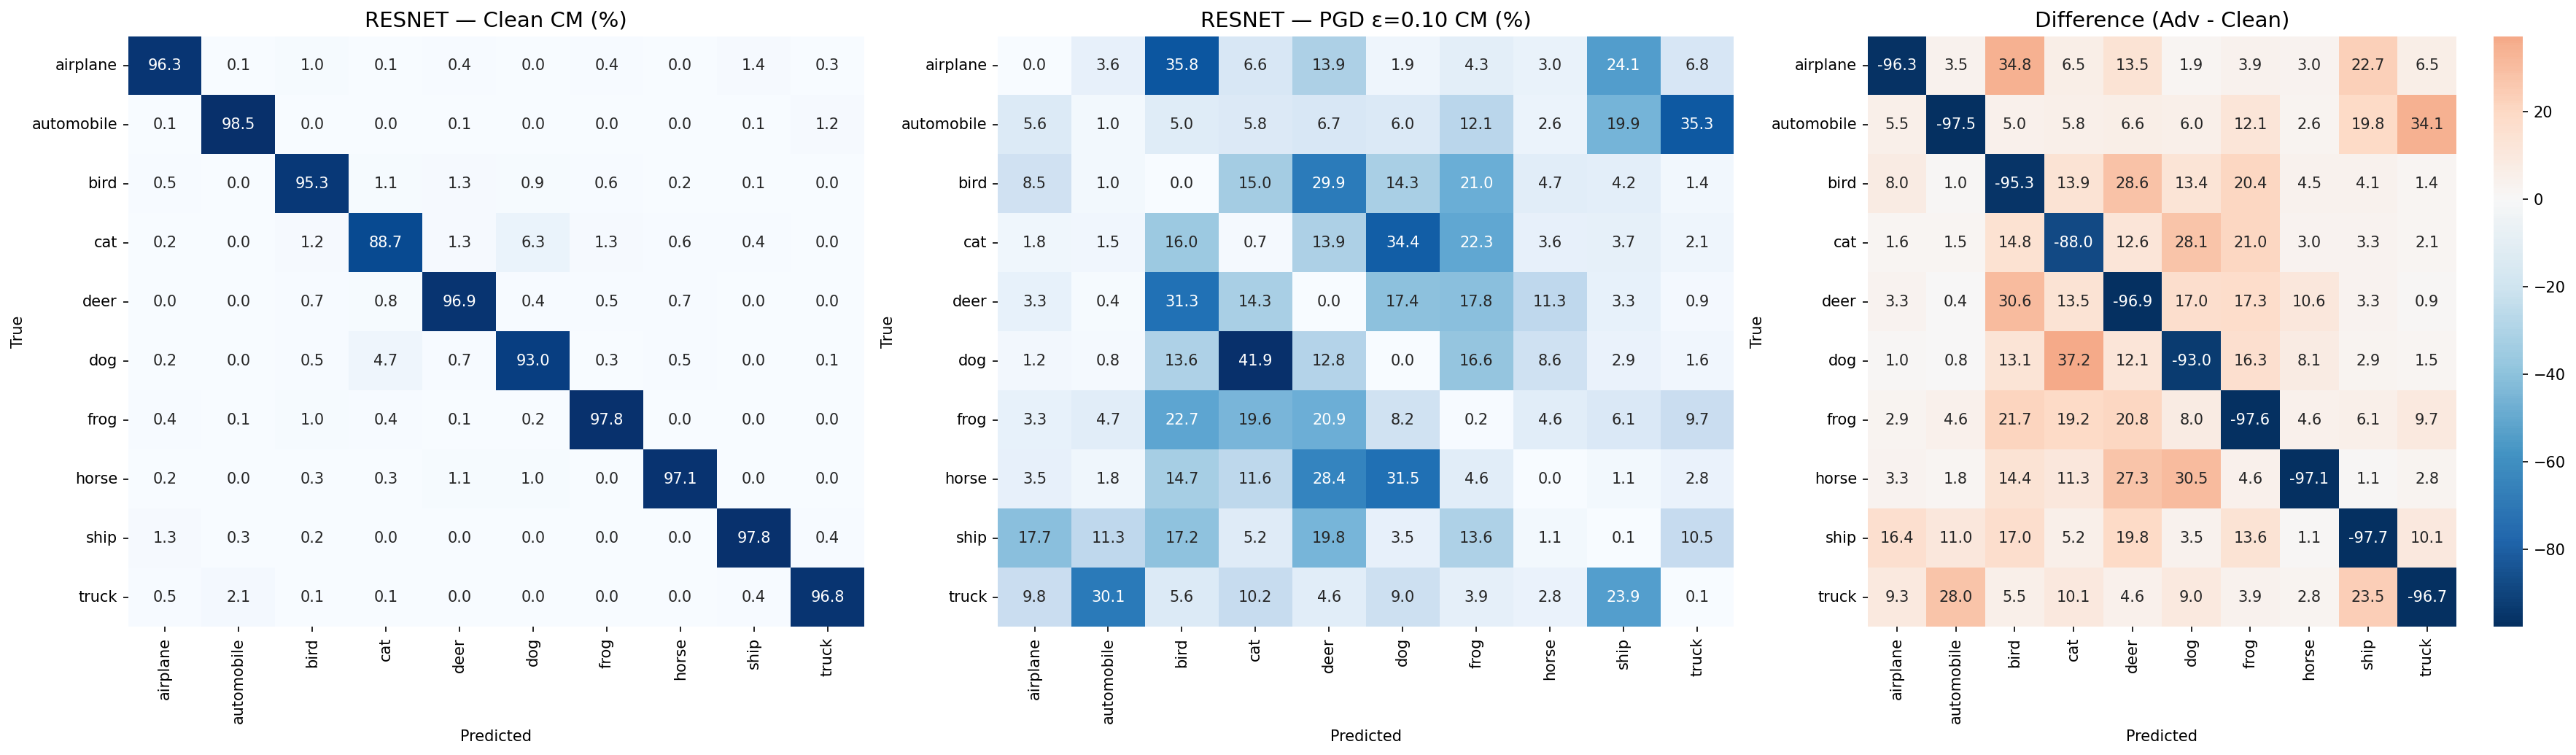
\includegraphics[width=\textwidth]{figures/resnet_confusion_suite.png}
  \caption{ResNet-18 (Fig.~A.14).}
\end{subfigure}
\hfill
\begin{subfigure}[b]{0.48\textwidth}
  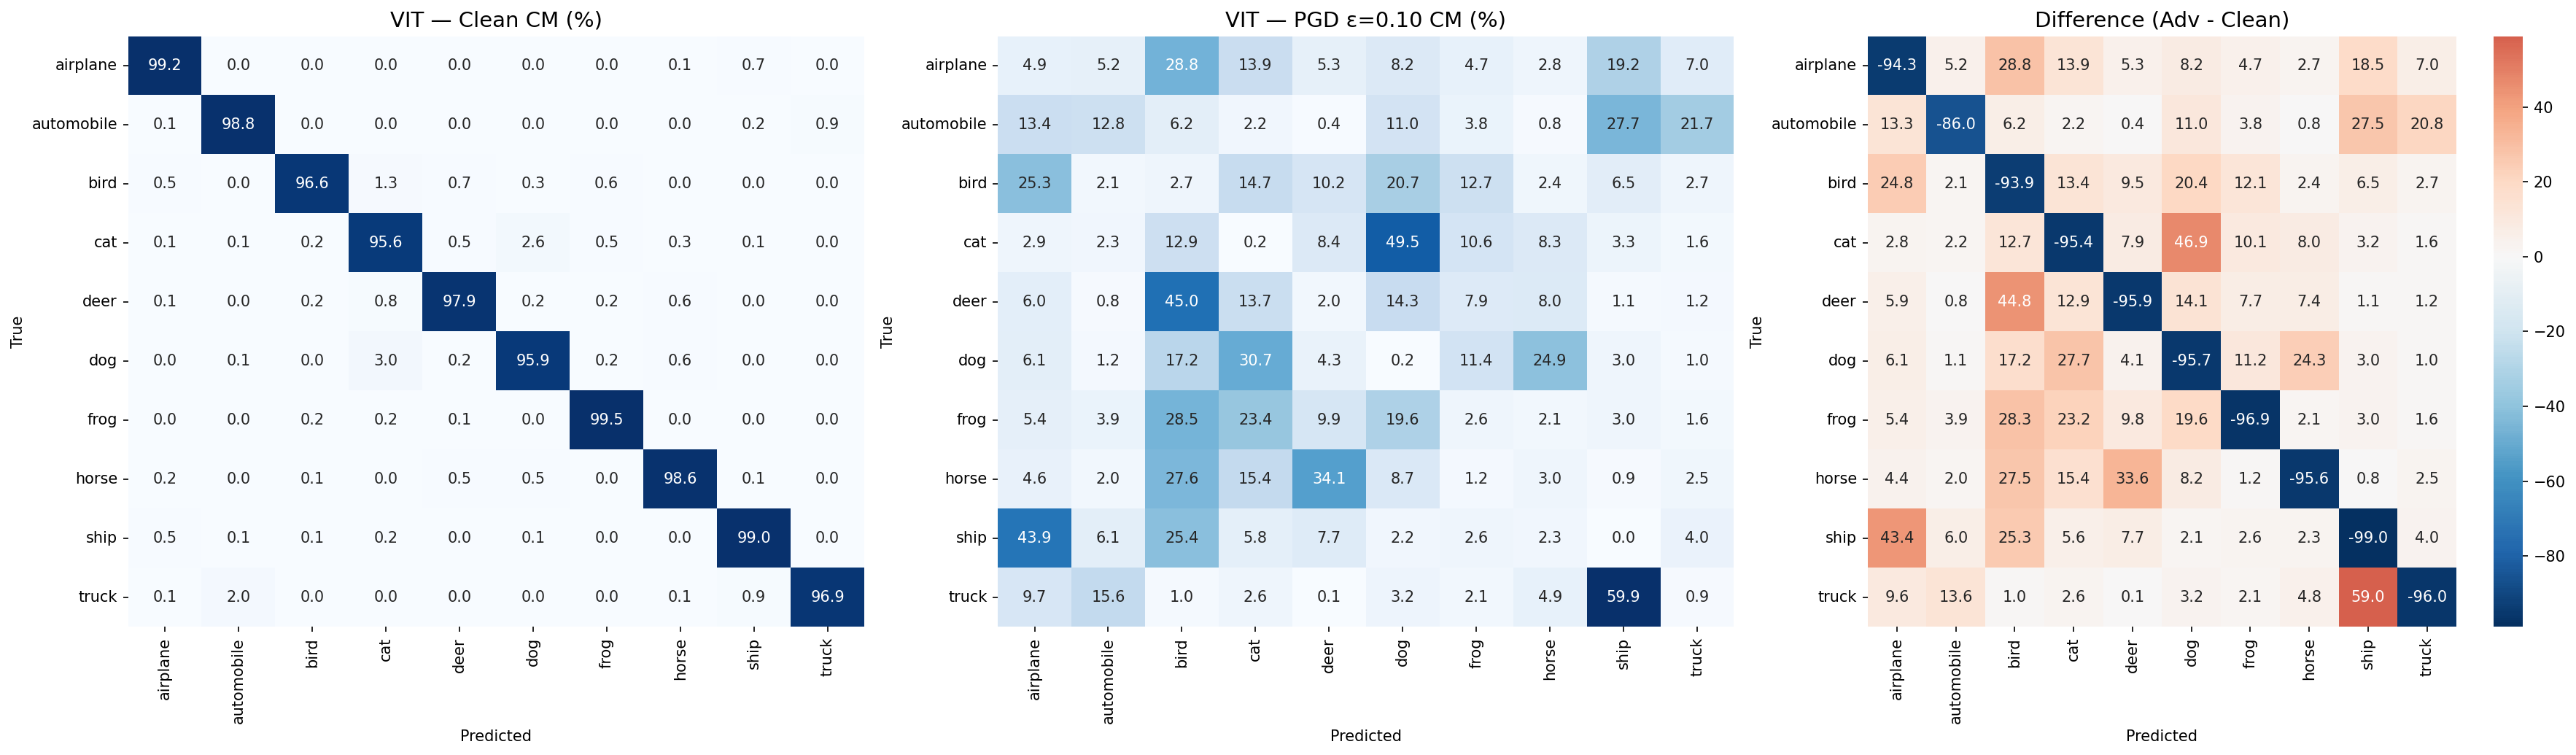
\includegraphics[width=\textwidth]{figures/vit_confusion_suite.png}
  \caption{ViT-Small (Fig.~A.15).}
\end{subfigure}
\caption{\textbf{Adversarial Confusion Matrices: ResNet-18 vs.\ ViT-Small}.}
\end{figure}

\begin{figure}[H]
\centering
\begin{subfigure}[b]{0.48\textwidth}
  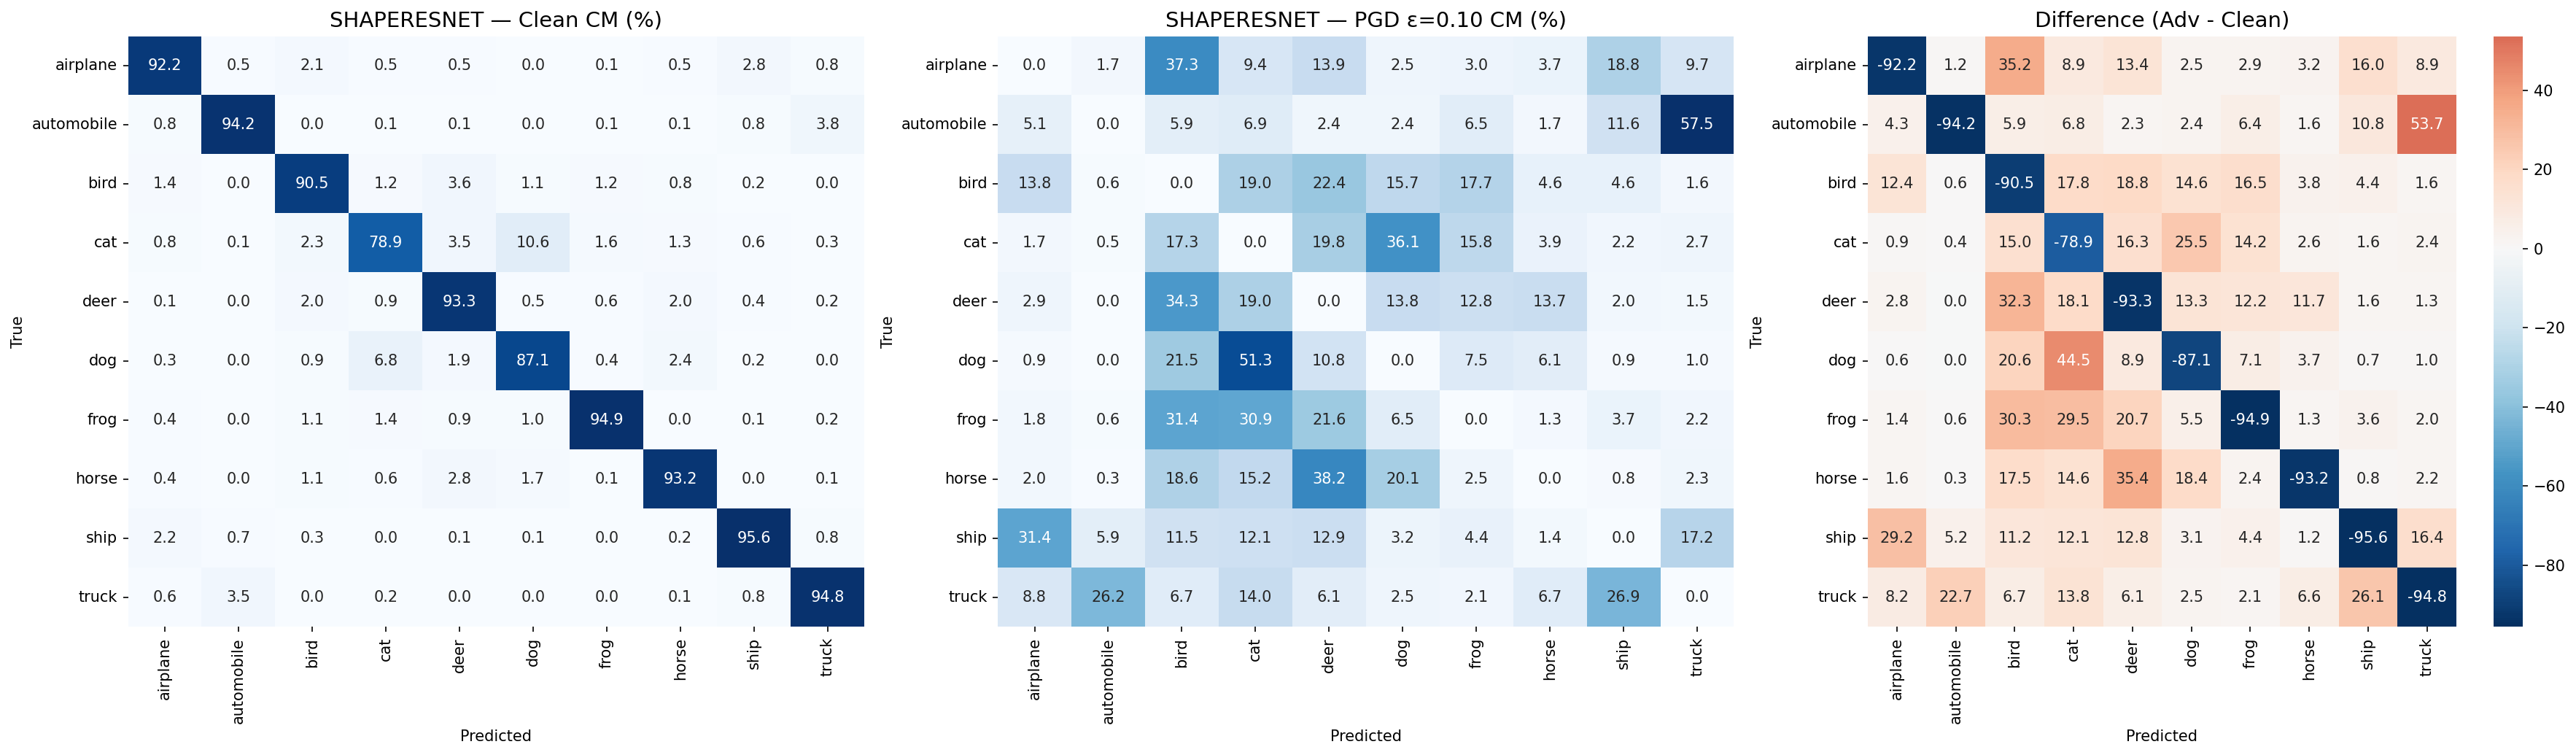
\includegraphics[width=\textwidth]{figures/shaperesnet_confusion_suite.png}
  \caption{Shape-ResNet-50 (Fig.~A.16).}
\end{subfigure}
\hfill
\begin{subfigure}[b]{0.48\textwidth}
  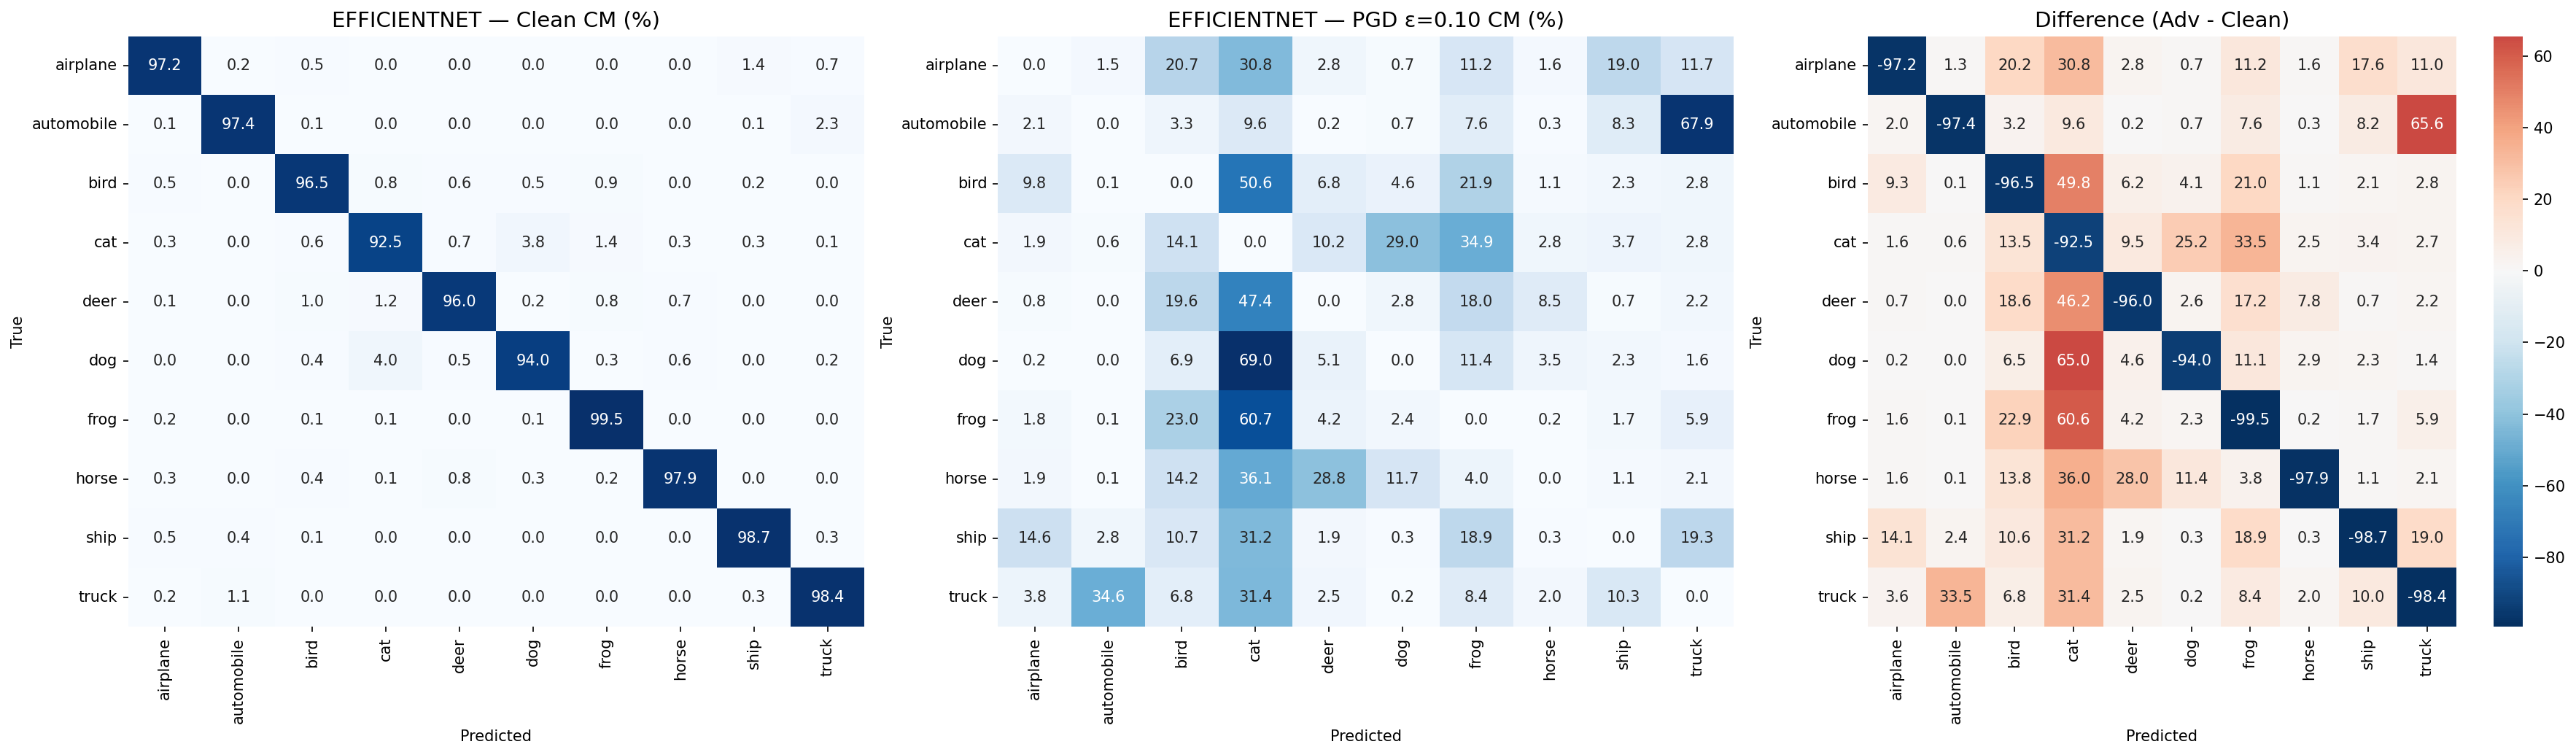
\includegraphics[width=\textwidth]{figures/efficientnet_confusion_suite.png}
  \caption{EfficientNet-B0 (Fig.~A.17).}
\end{subfigure}
\caption{\textbf{Alternative Feedforward Confusion Suites}.}
\end{figure}

\begin{figure}[H]
\centering
\begin{subfigure}[b]{0.48\textwidth}
  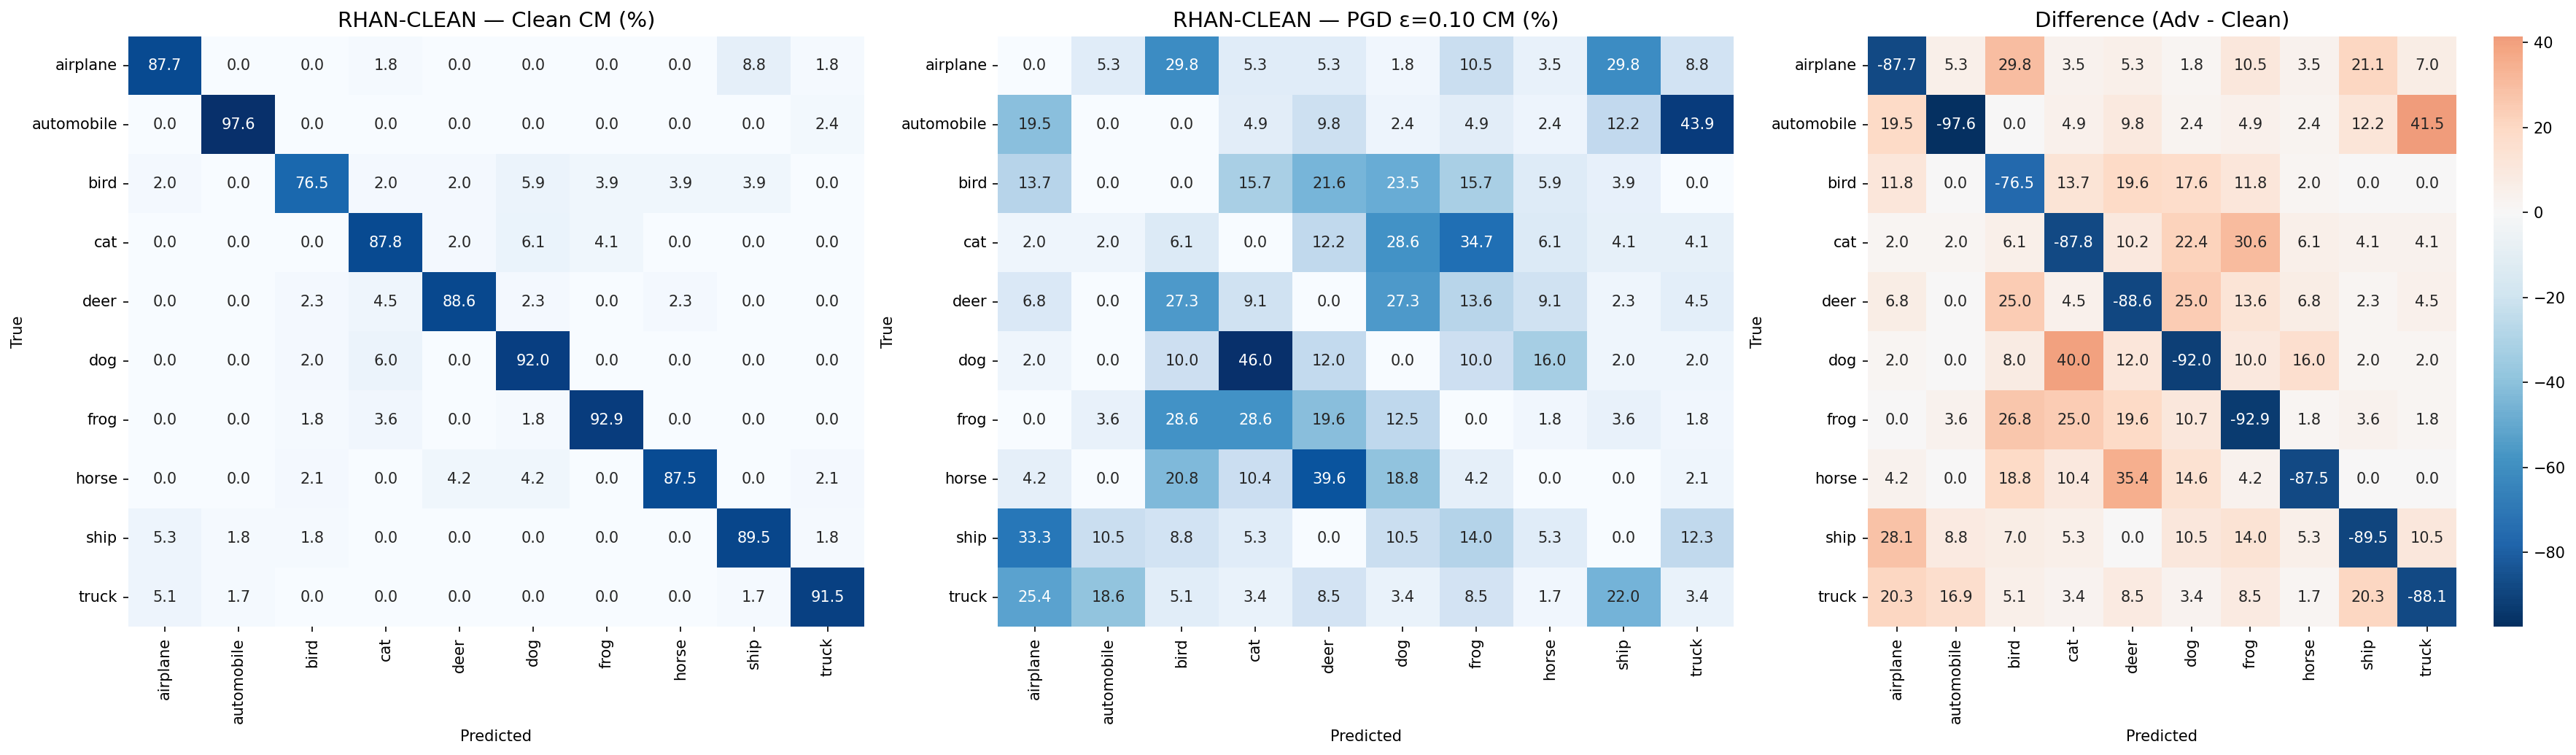
\includegraphics[width=\textwidth]{figures/rhan-clean_confusion_suite.png}
  \caption{RHAN-clean (Fig.~A.18).}
\end{subfigure}
\hfill
\begin{subfigure}[b]{0.48\textwidth}
  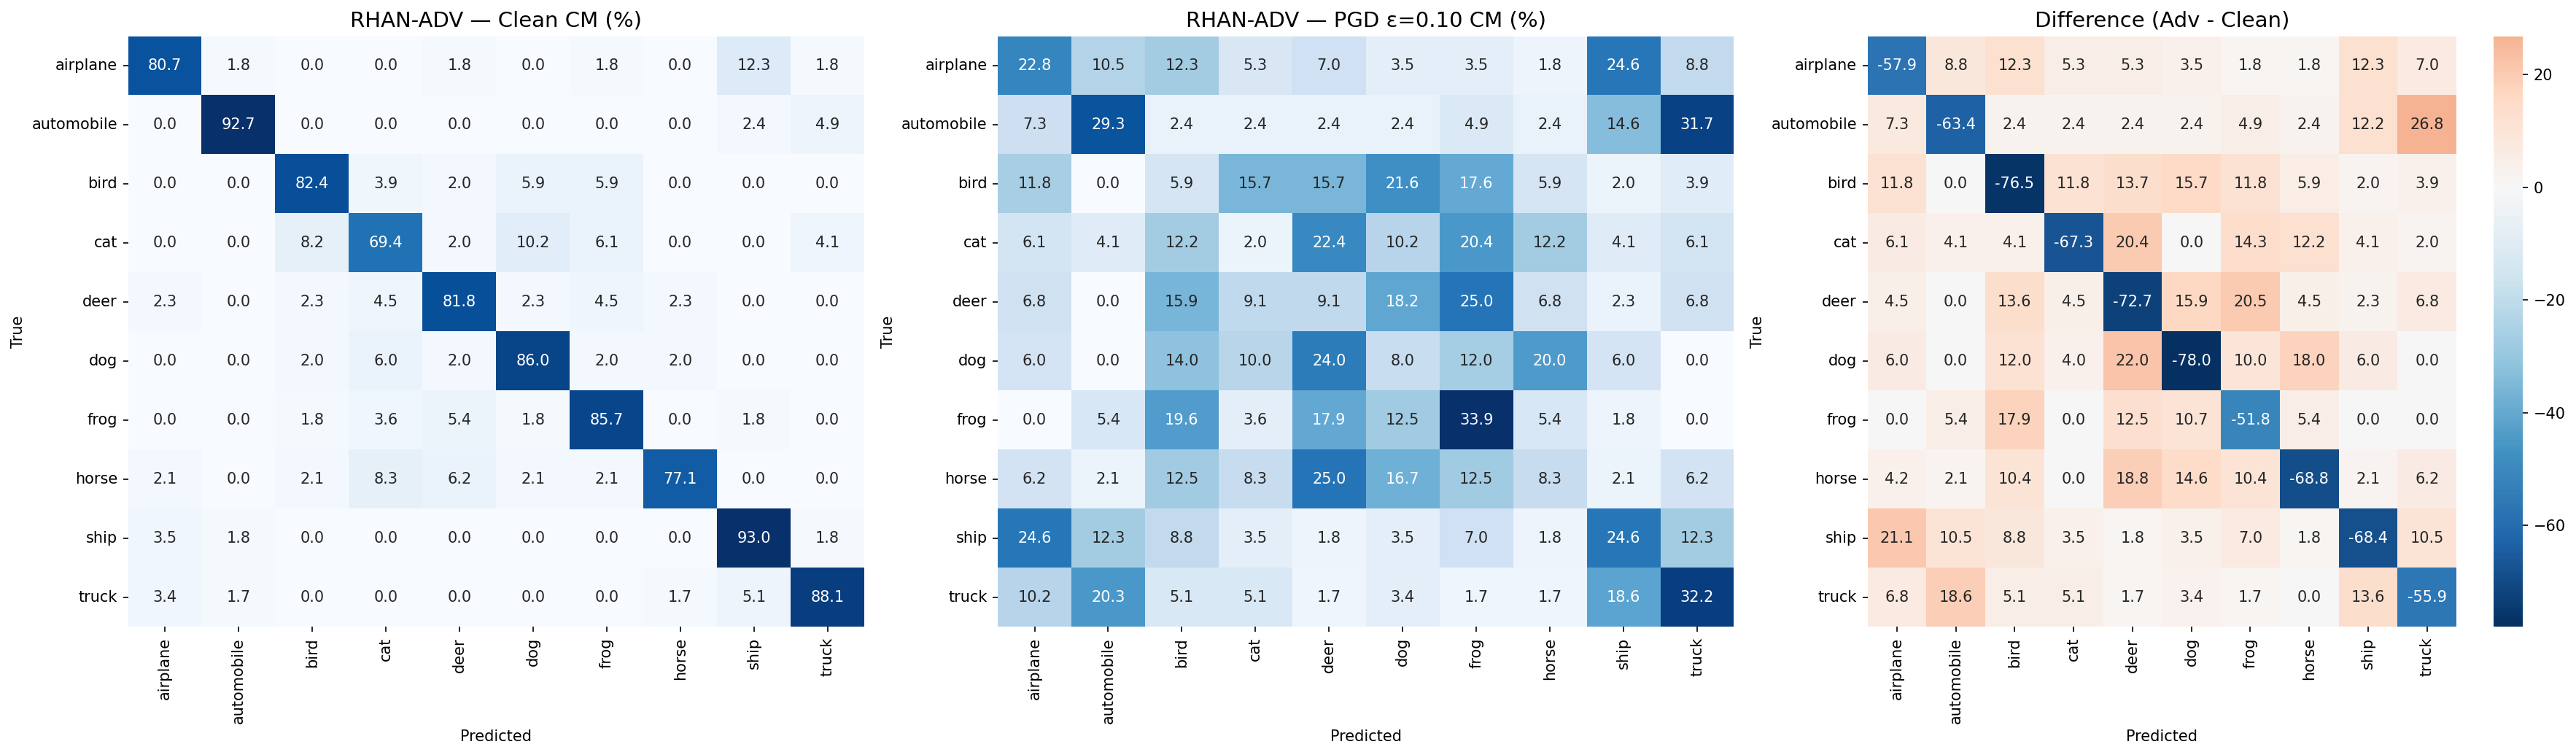
\includegraphics[width=\textwidth]{figures/rhan-adv_confusion_suite.png}
  \caption{RHAN-adv (Fig.~A.19).}
\end{subfigure}
\caption{\textbf{RHAN Confusion Suite Comparison}.}
\end{figure}


% ============================================================
\section{Recurrent Feedback Gating Maps}
\label{app:gating}
% ============================================================

\begin{figure}[H]
\centering
\begin{subfigure}[b]{0.48\textwidth}
  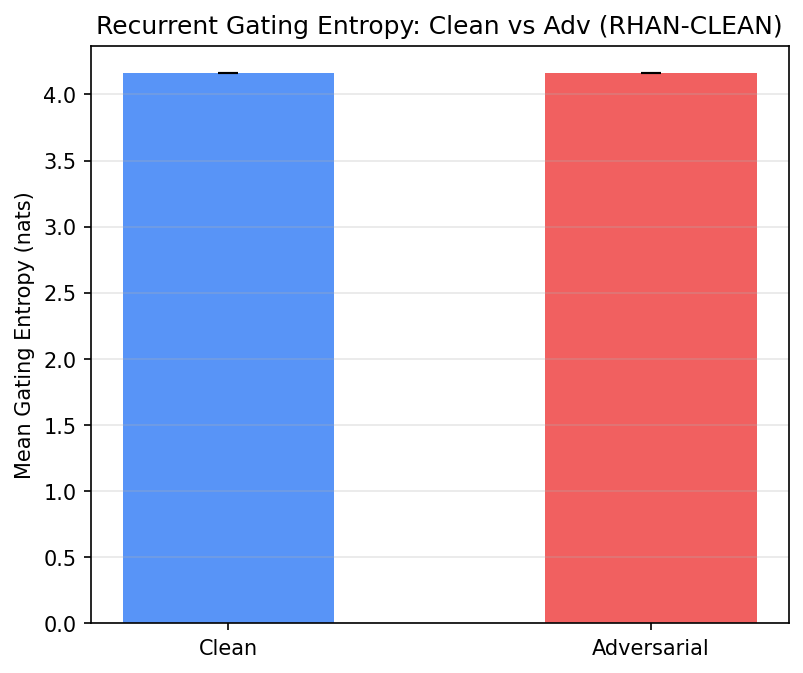
\includegraphics[width=\textwidth]{figures/gating_entropy_comparison.png}
  \caption{Gate Entropy (Fig.~A.20).}
\end{subfigure}
\hfill
\begin{subfigure}[b]{0.48\textwidth}
  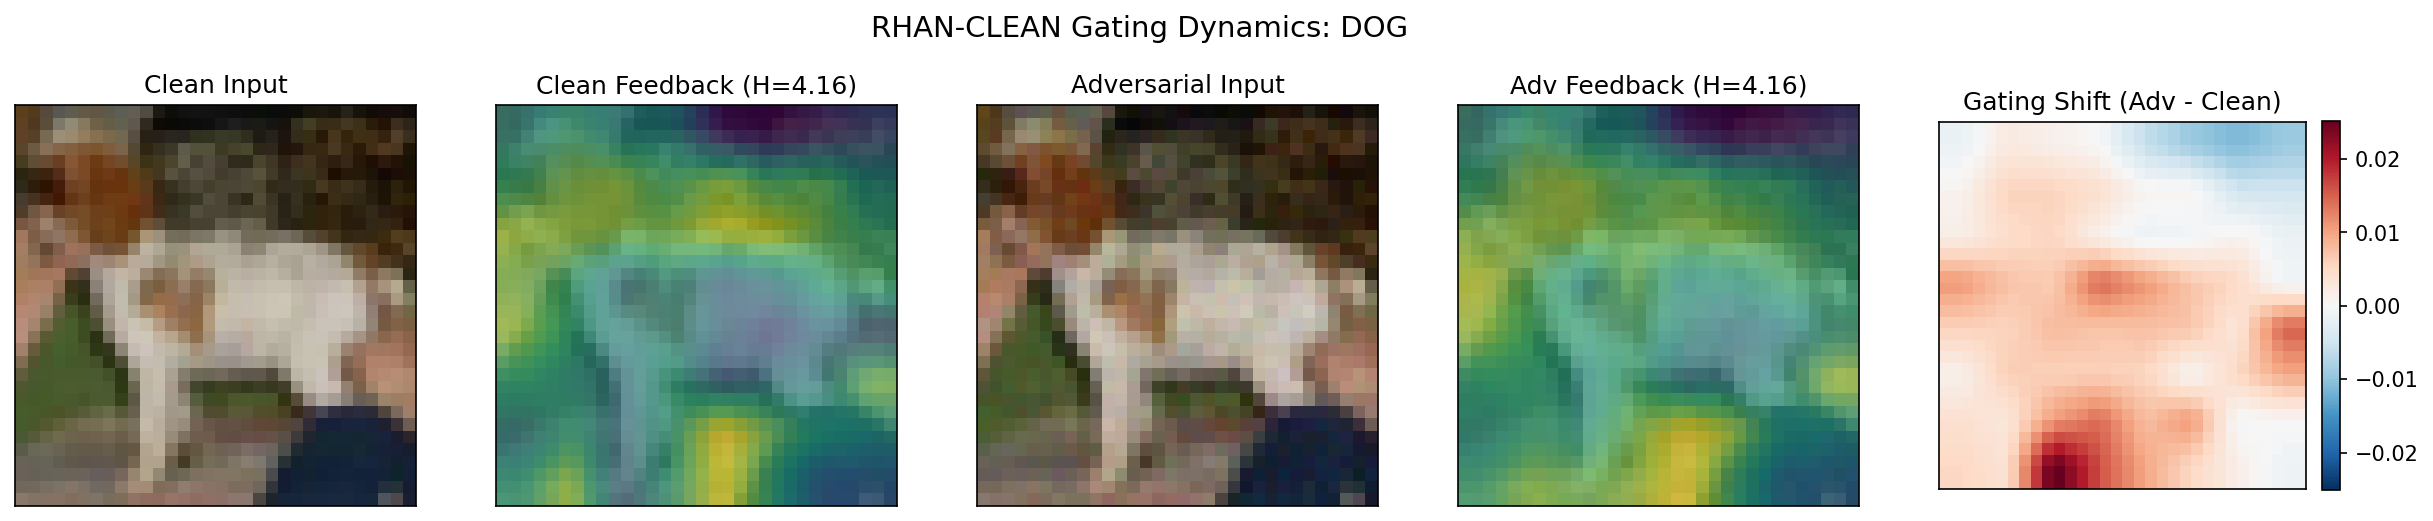
\includegraphics[width=\textwidth]{figures/feedback_dog.png}
  \caption{Dog Gating Map (Fig.~A.21).}
\end{subfigure}
\caption{\textbf{RHAN-adv Gating Dynamics}.}
\end{figure}

\begin{figure}[H]
\centering
\begin{subfigure}[b]{0.48\textwidth}
  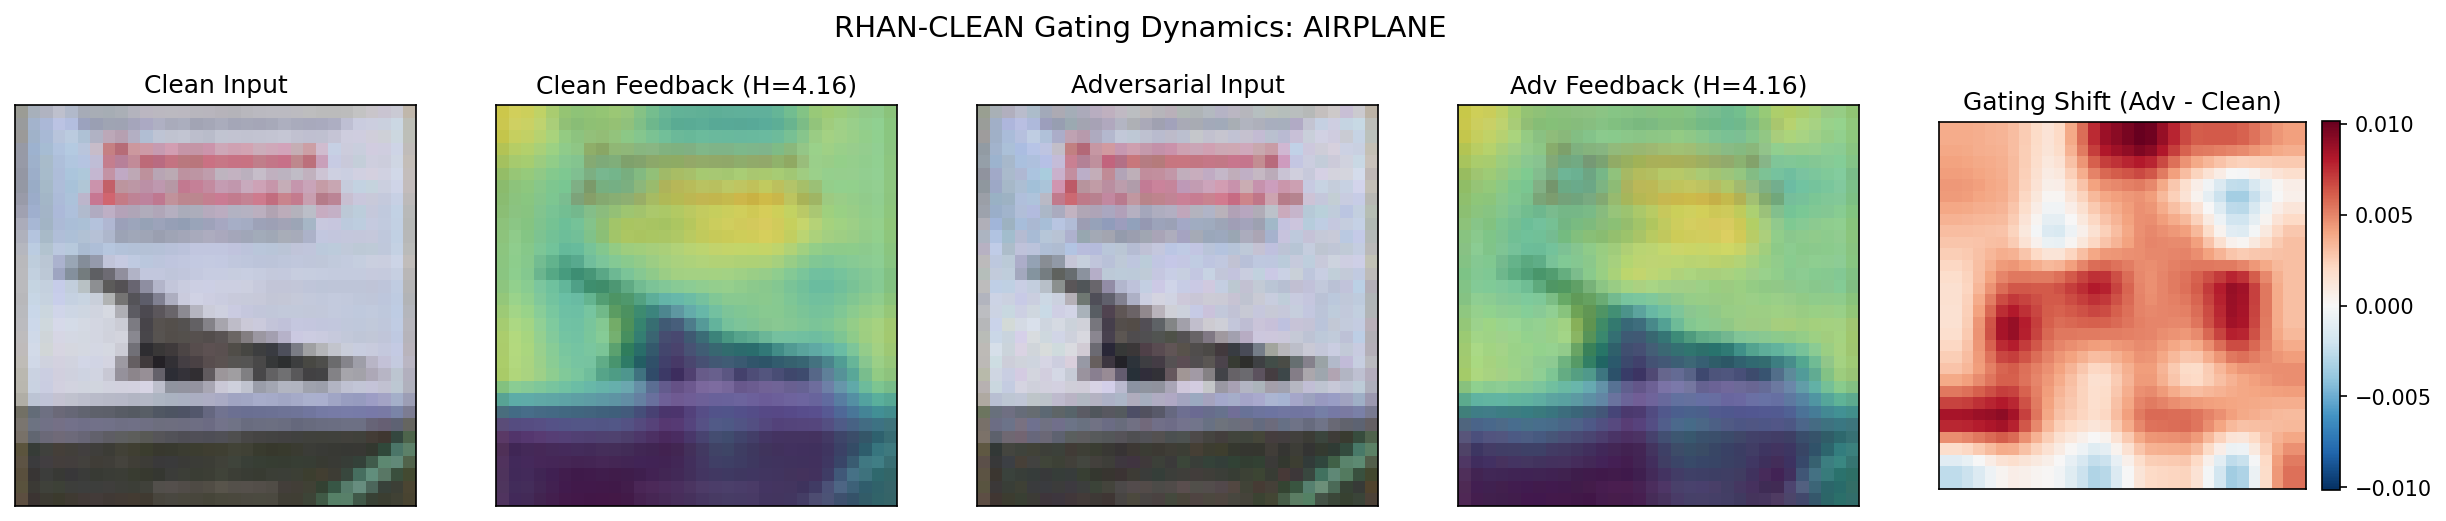
\includegraphics[width=\textwidth]{figures/feedback_airplane.png}
  \caption{Airplane (Fig.~A.22).}
\end{subfigure}
\hfill
\begin{subfigure}[b]{0.48\textwidth}
  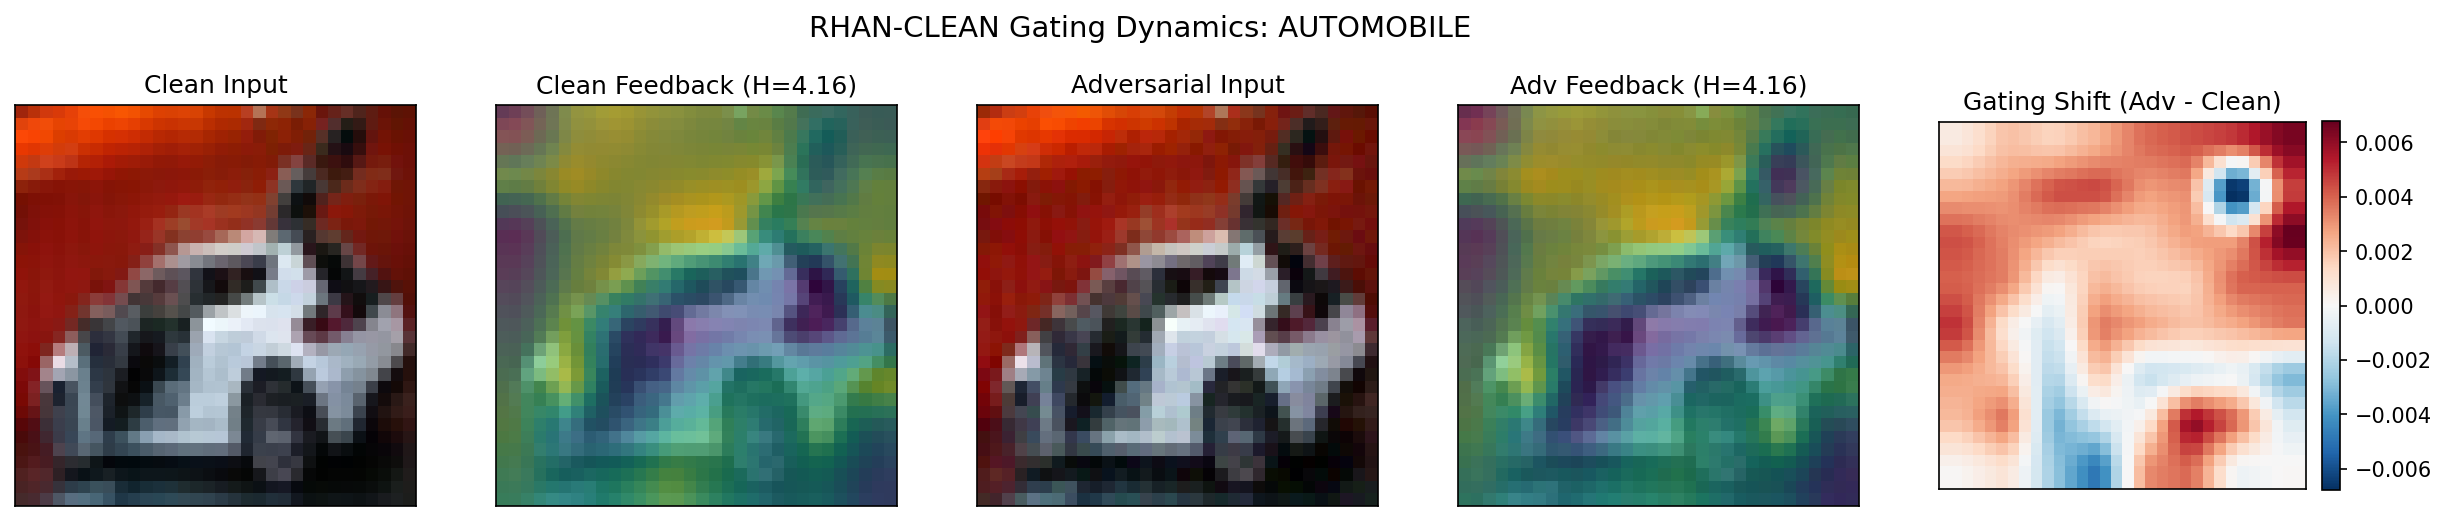
\includegraphics[width=\textwidth]{figures/feedback_automobile.png}
  \caption{Automobile (Fig.~A.23).}
\end{subfigure}
\caption{\textbf{Gating Maps: Airplane and Automobile}.}
\end{figure}

\begin{figure}[H]
\centering
\begin{subfigure}[b]{0.48\textwidth}
  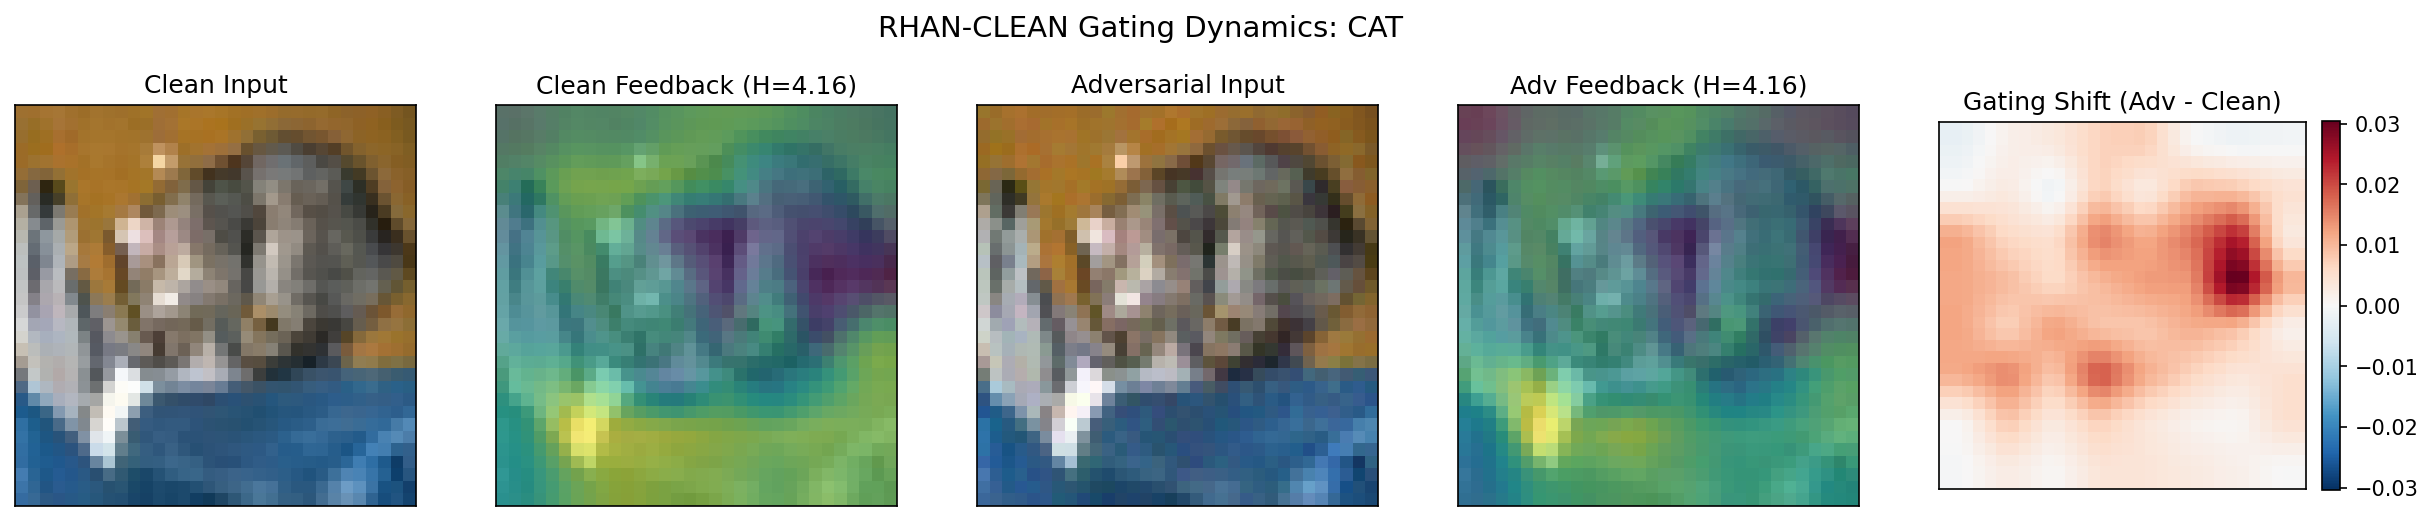
\includegraphics[width=\textwidth]{figures/feedback_cat.png}
  \caption{Cat (Fig.~A.24).}
\end{subfigure}
\hfill
\begin{subfigure}[b]{0.48\textwidth}
  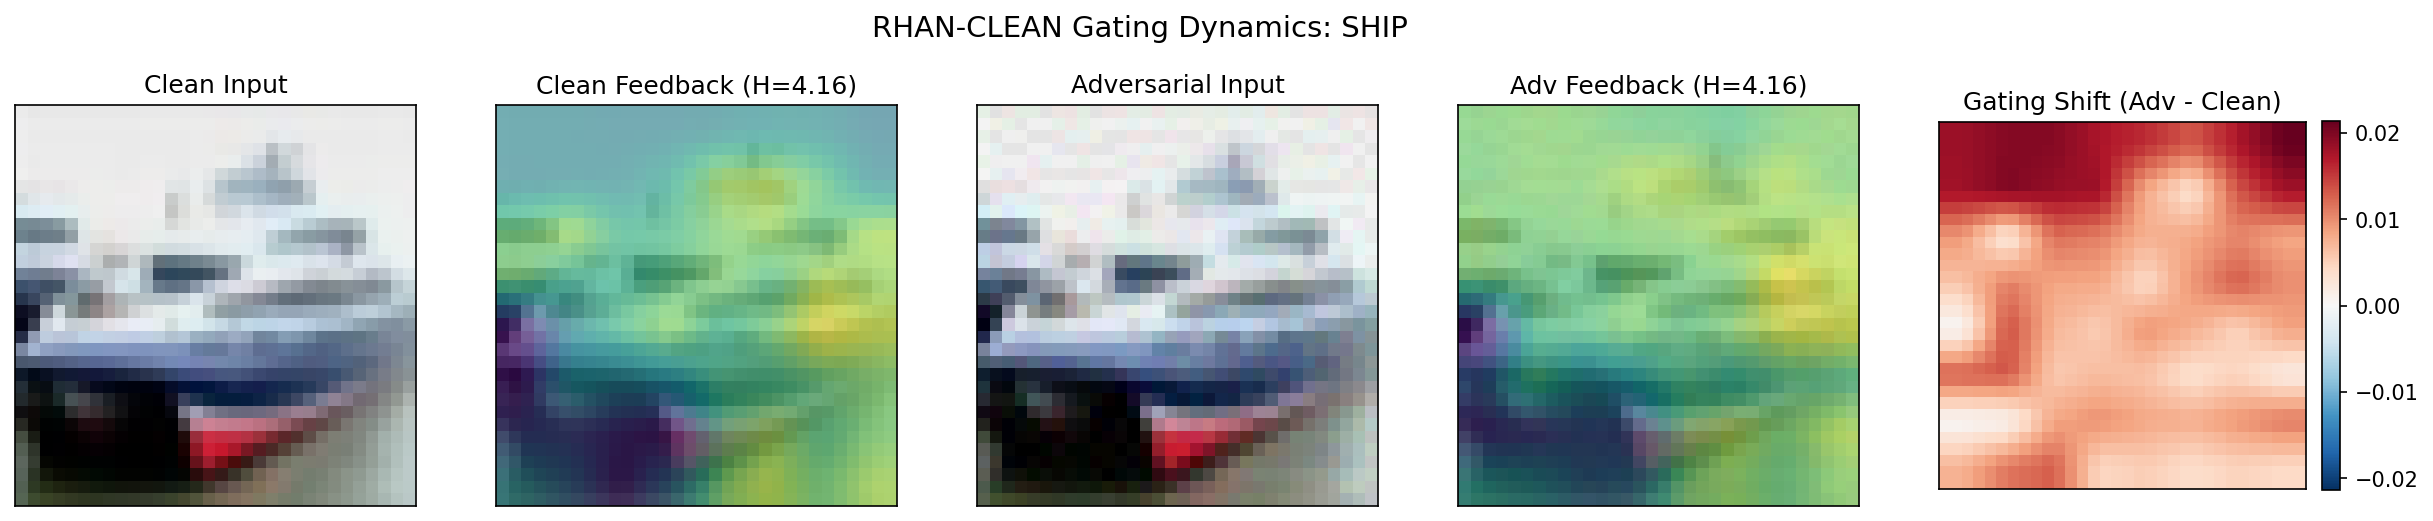
\includegraphics[width=\textwidth]{figures/feedback_ship.png}
  \caption{Ship (Fig.~A.25).}
\end{subfigure}
\caption{\textbf{Gating Maps: Cat and Ship}.}
\end{figure}


% ============================================================
\section{Visual Psychophysics Stimuli and Grad-CAM Explanations}
\label{app:gradcam}
% ============================================================

\begin{figure}[H]
\centering
\begin{subfigure}[b]{0.32\textwidth}
  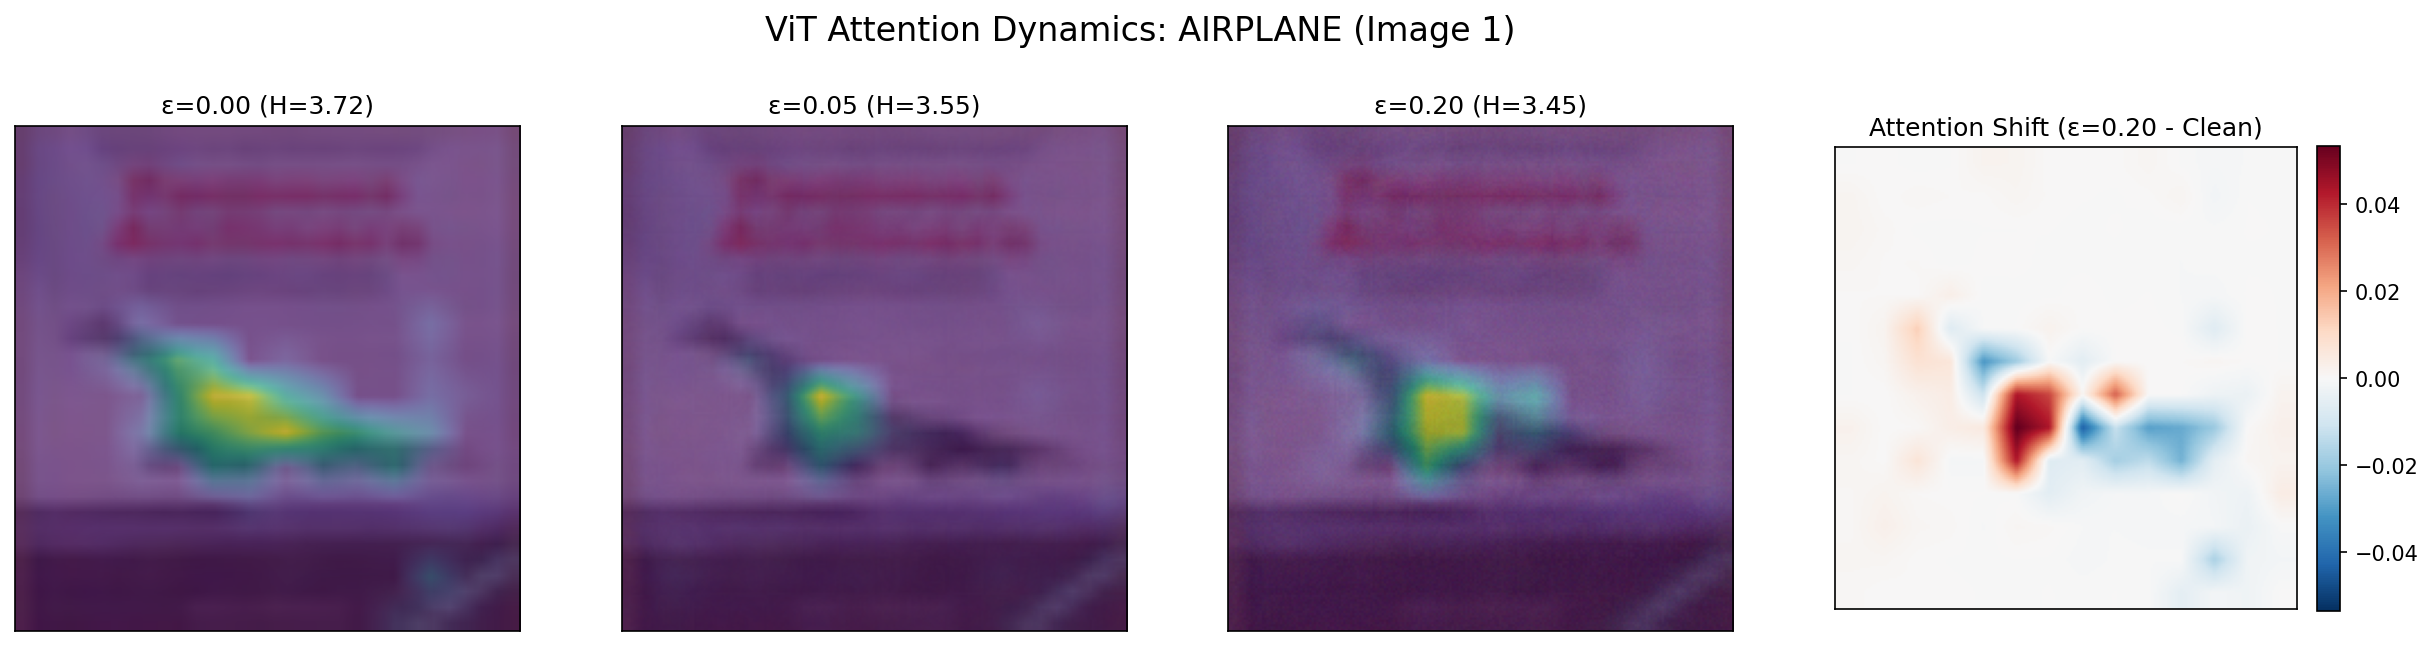
\includegraphics[width=\textwidth]{figures/airplane_1.png}
  \caption{Clean}
\end{subfigure}
\hfill
\begin{subfigure}[b]{0.32\textwidth}
  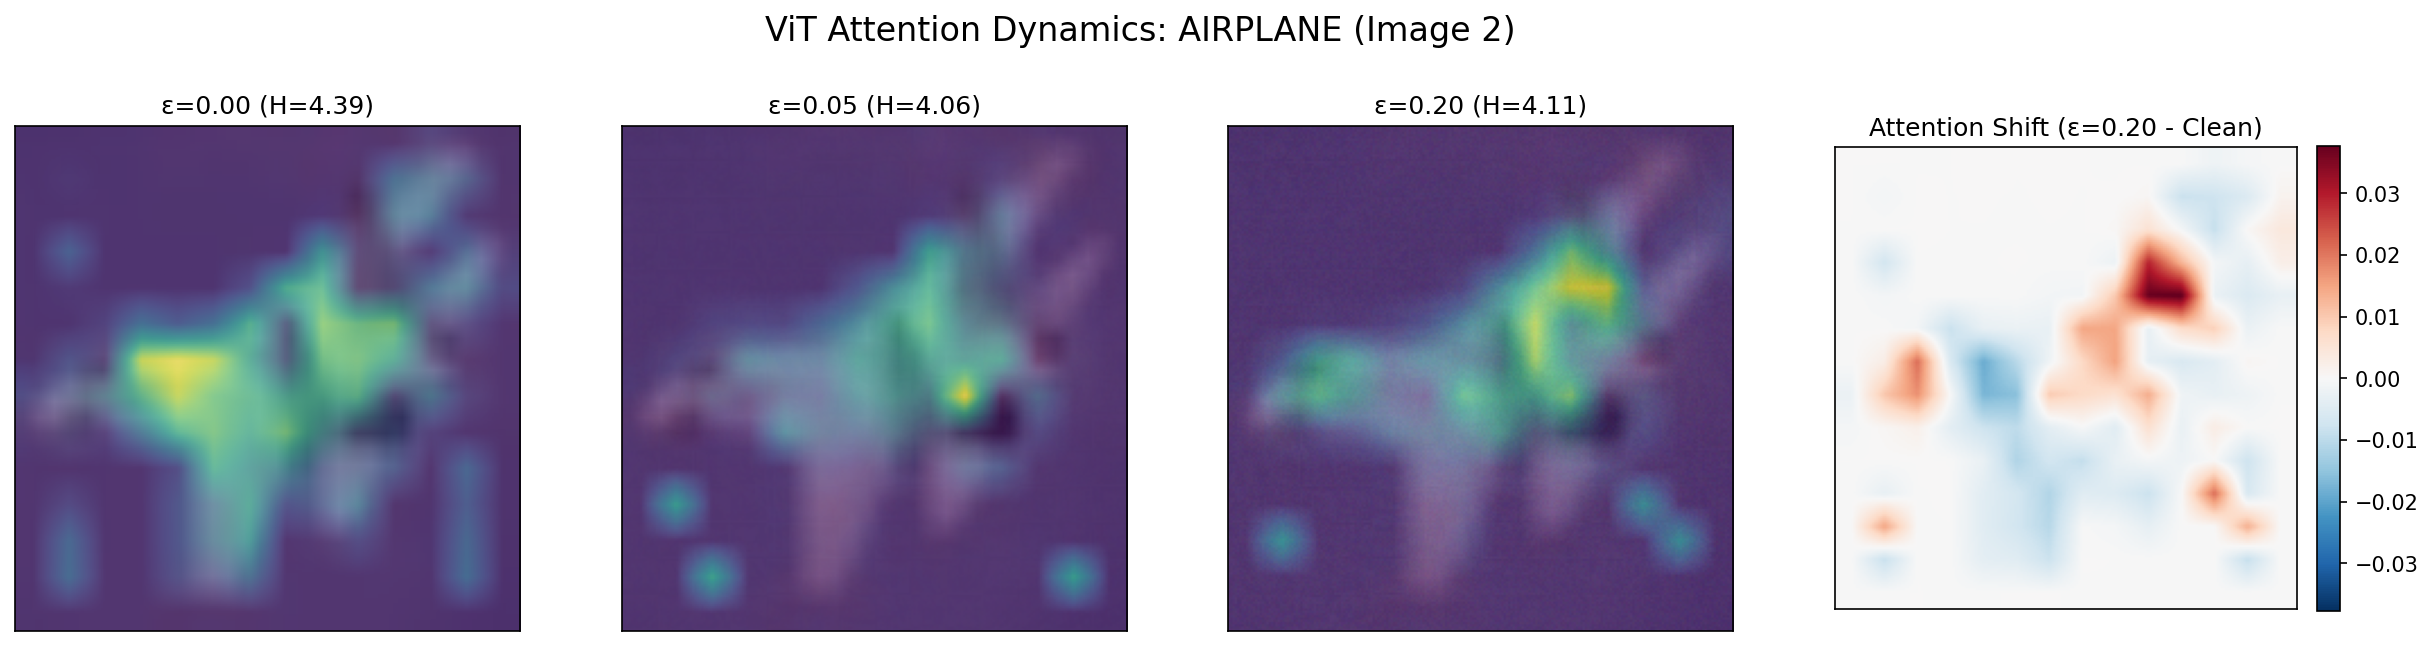
\includegraphics[width=\textwidth]{figures/airplane_2.png}
  \caption{Adversarial}
\end{subfigure}
\hfill
\begin{subfigure}[b]{0.32\textwidth}
  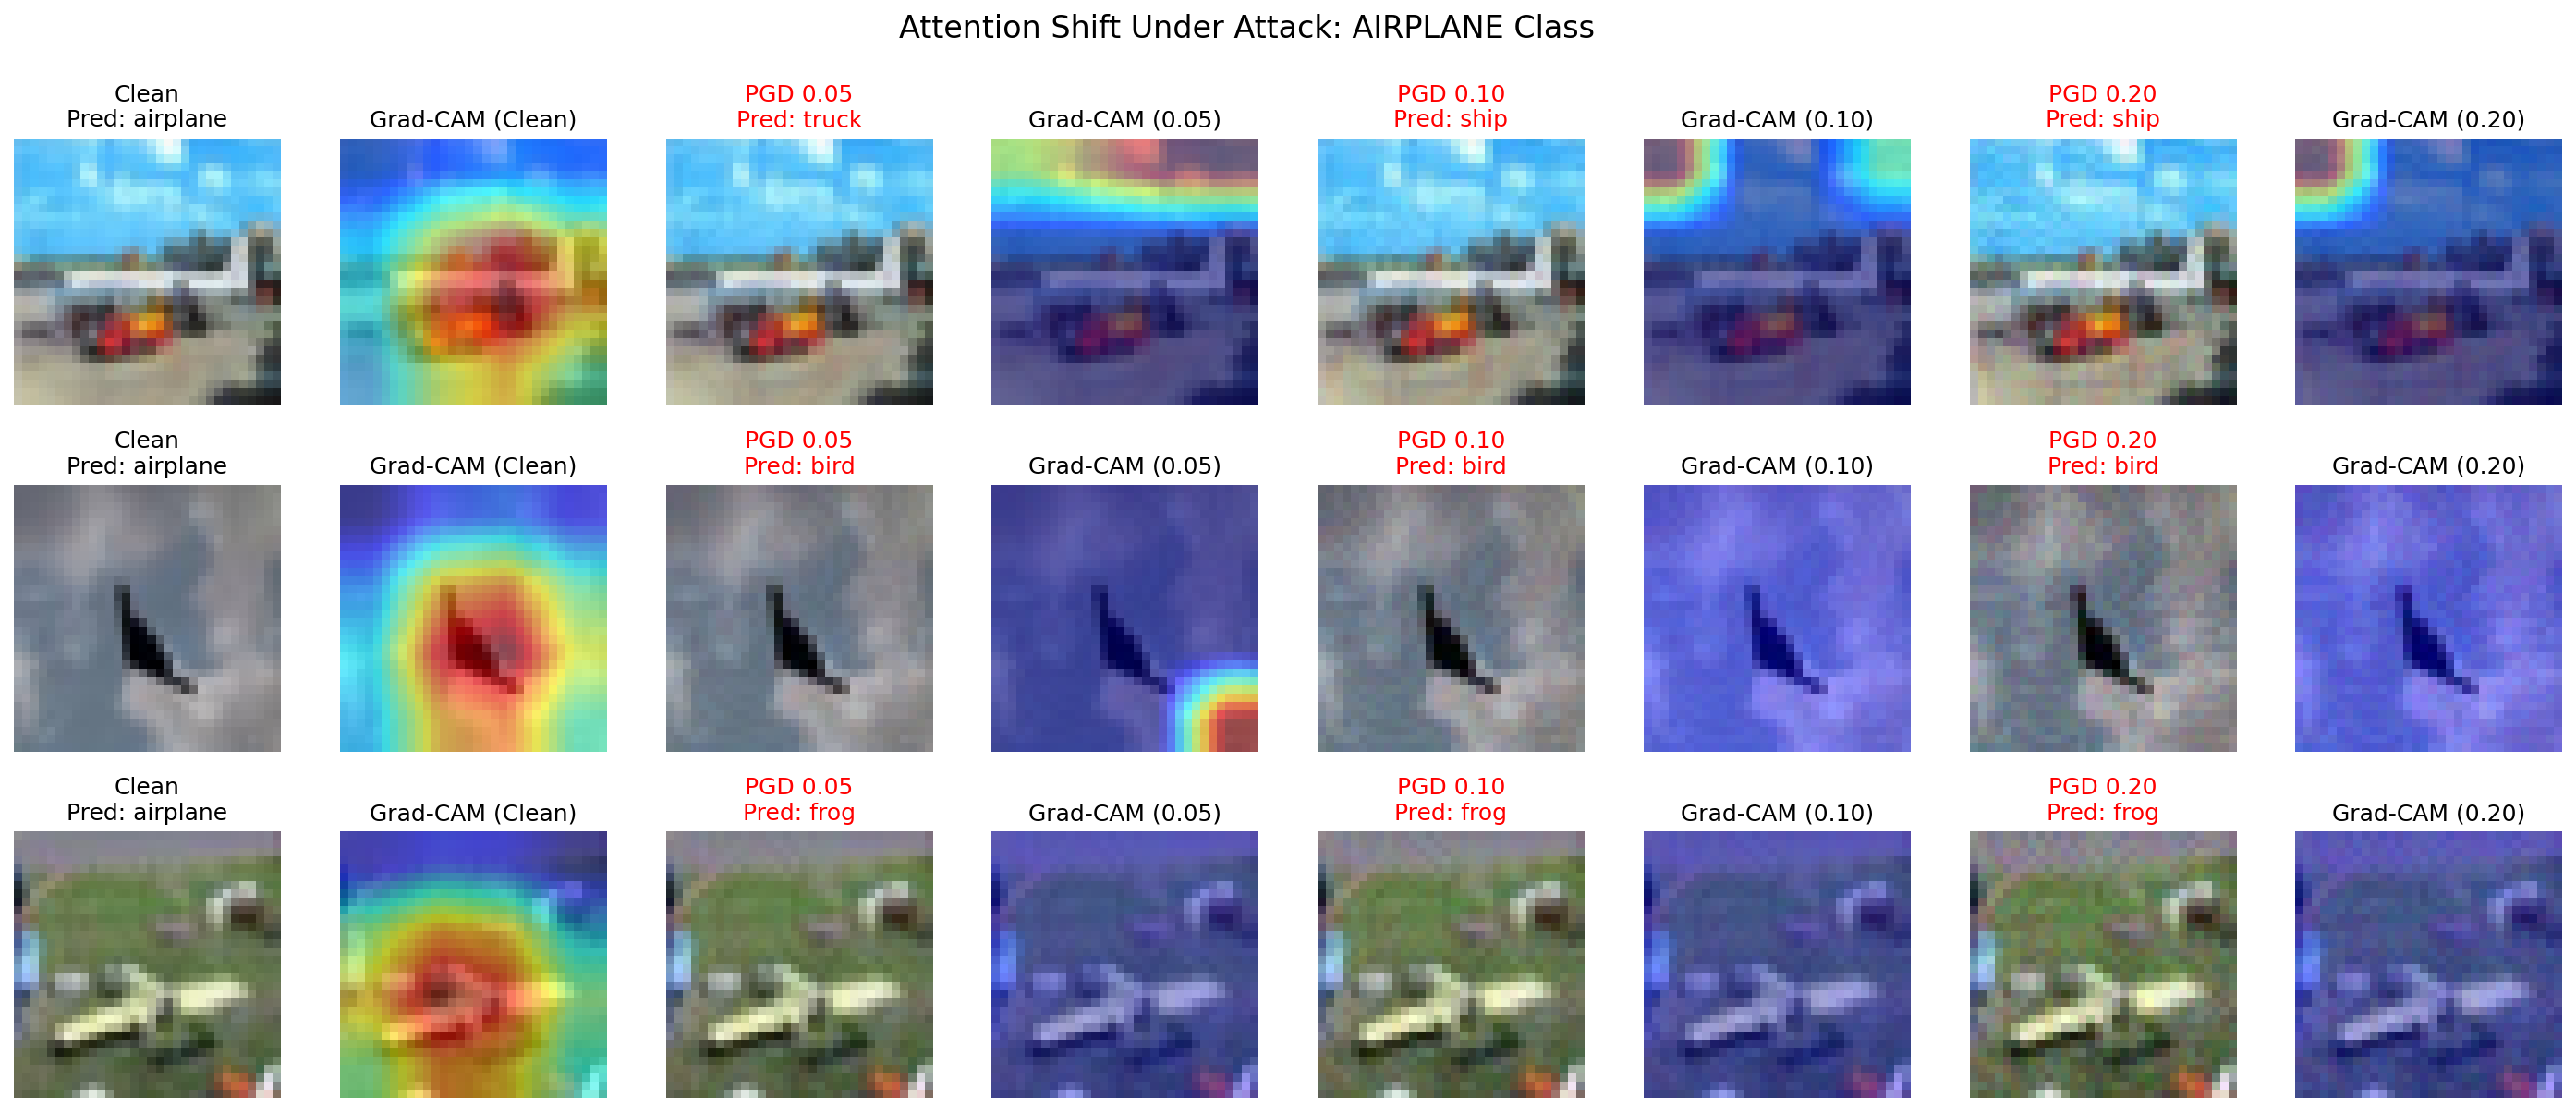
\includegraphics[width=\textwidth]{figures/airplane_gradcam.png}
  \caption{Grad-CAM}
\end{subfigure}
\caption{\textbf{Airplane Stimuli and Grad-CAM (Fig.~A.26, A.27)}.}
\end{figure}

\begin{figure}[H]
\centering
\begin{subfigure}[b]{0.32\textwidth}
  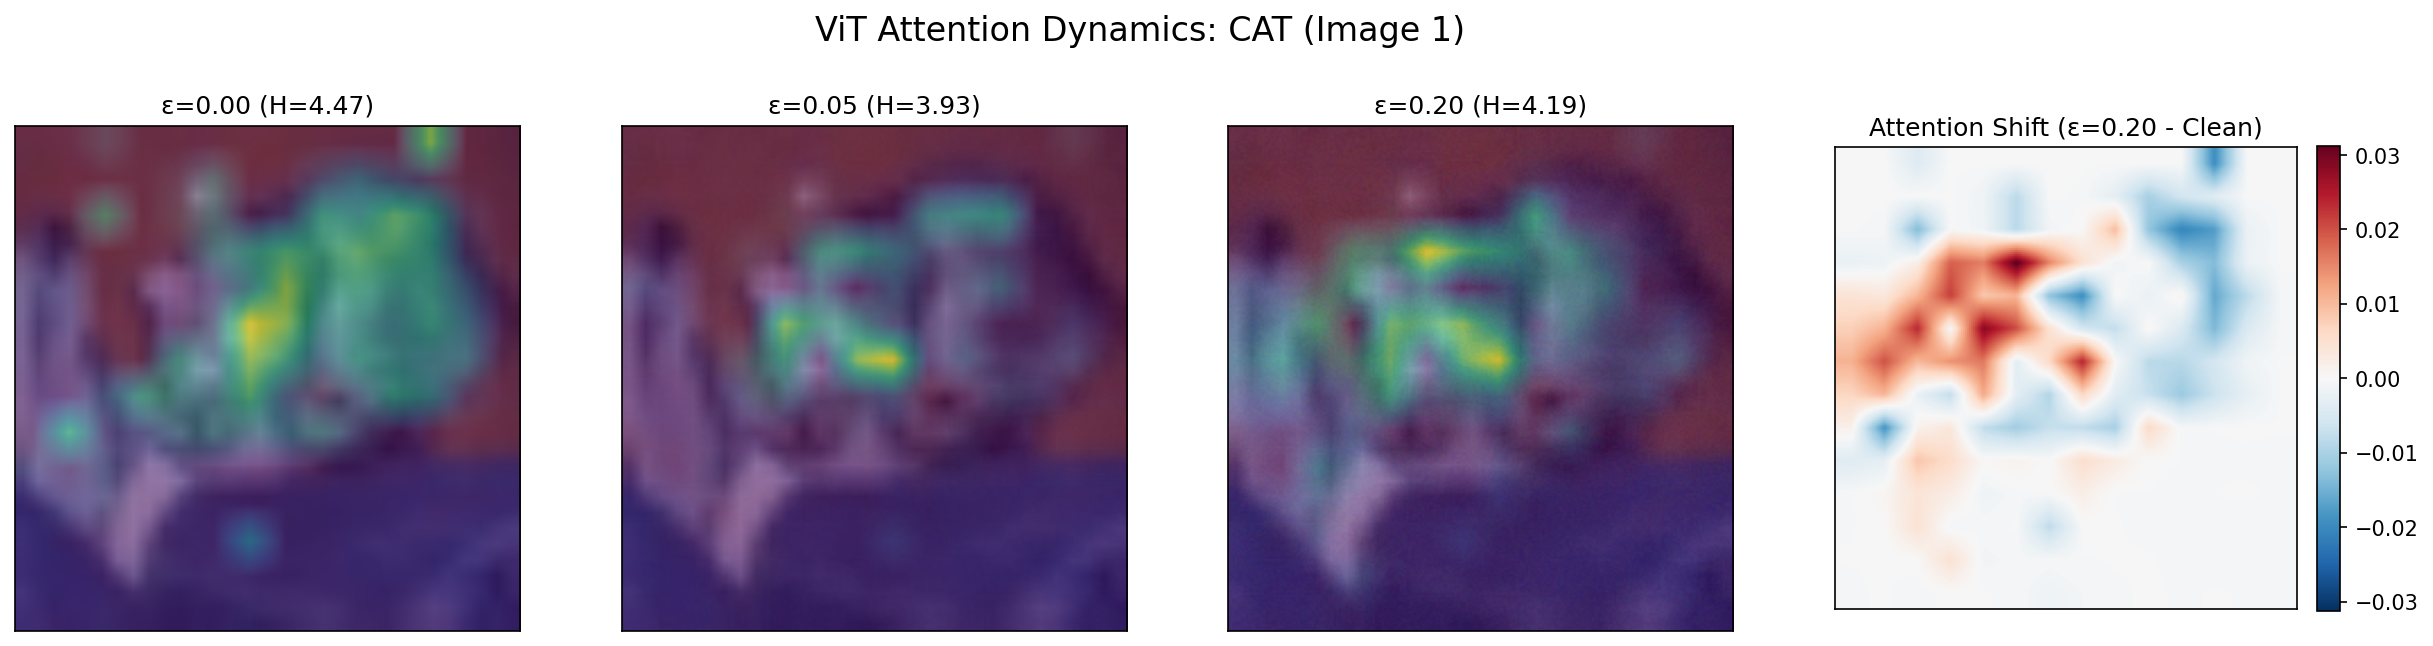
\includegraphics[width=\textwidth]{figures/cat_1.png}
  \caption{Clean}
\end{subfigure}
\hfill
\begin{subfigure}[b]{0.32\textwidth}
  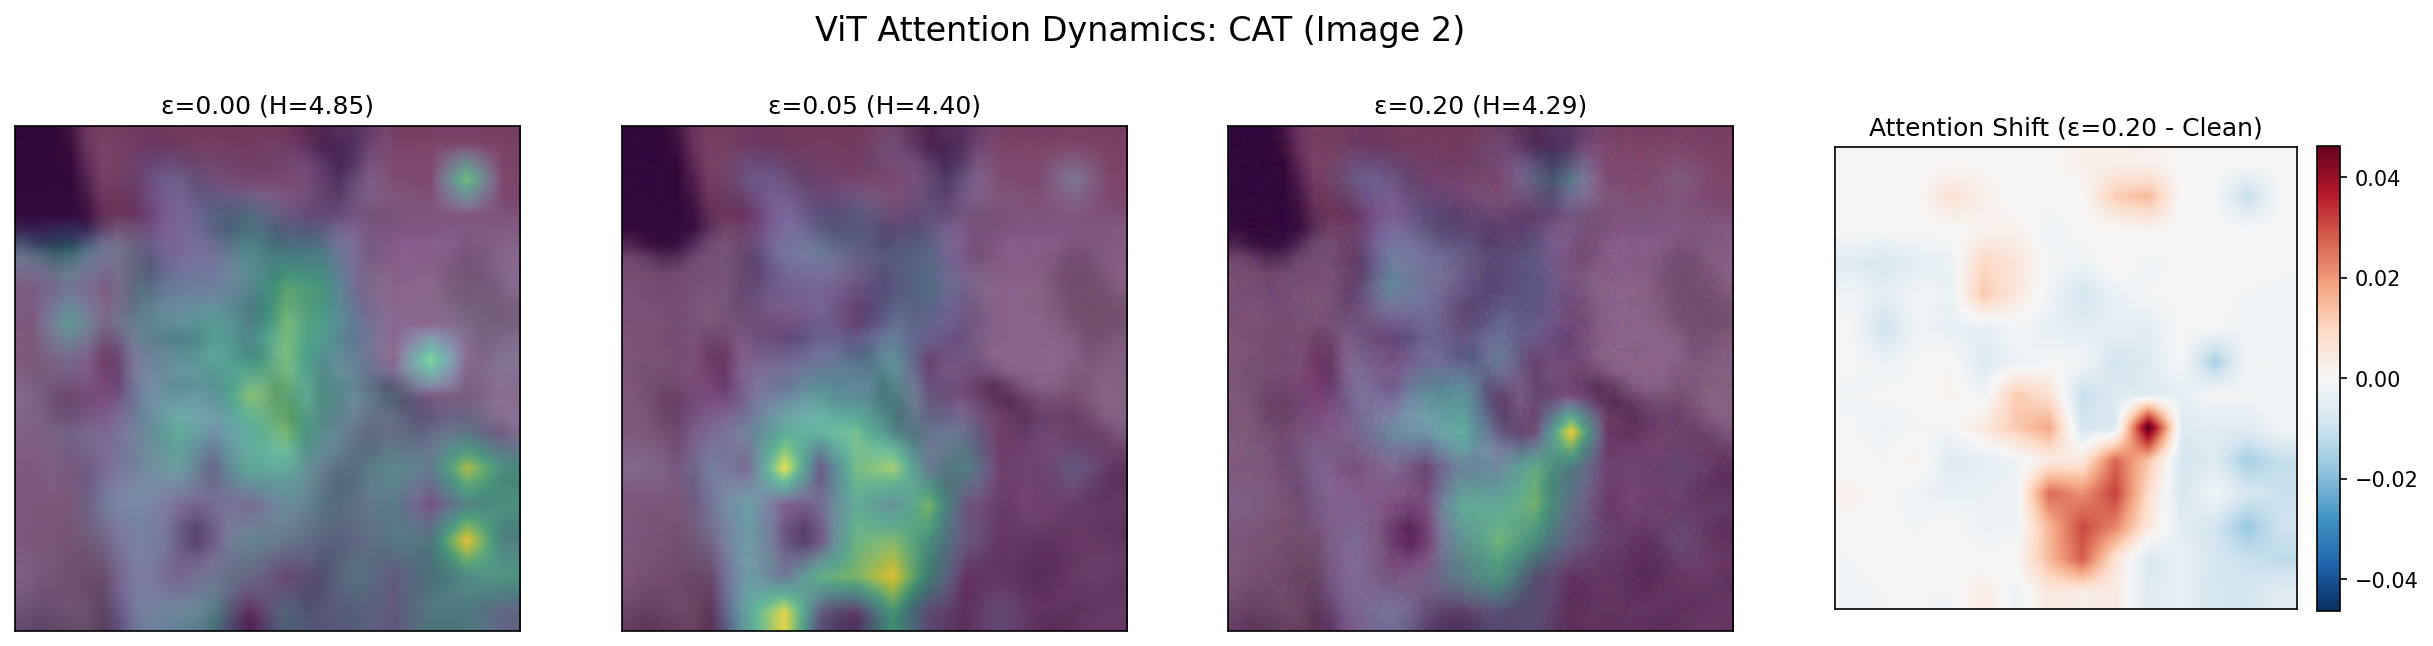
\includegraphics[width=\textwidth]{figures/cat_2.png}
  \caption{Adversarial}
\end{subfigure}
\hfill
\begin{subfigure}[b]{0.32\textwidth}
  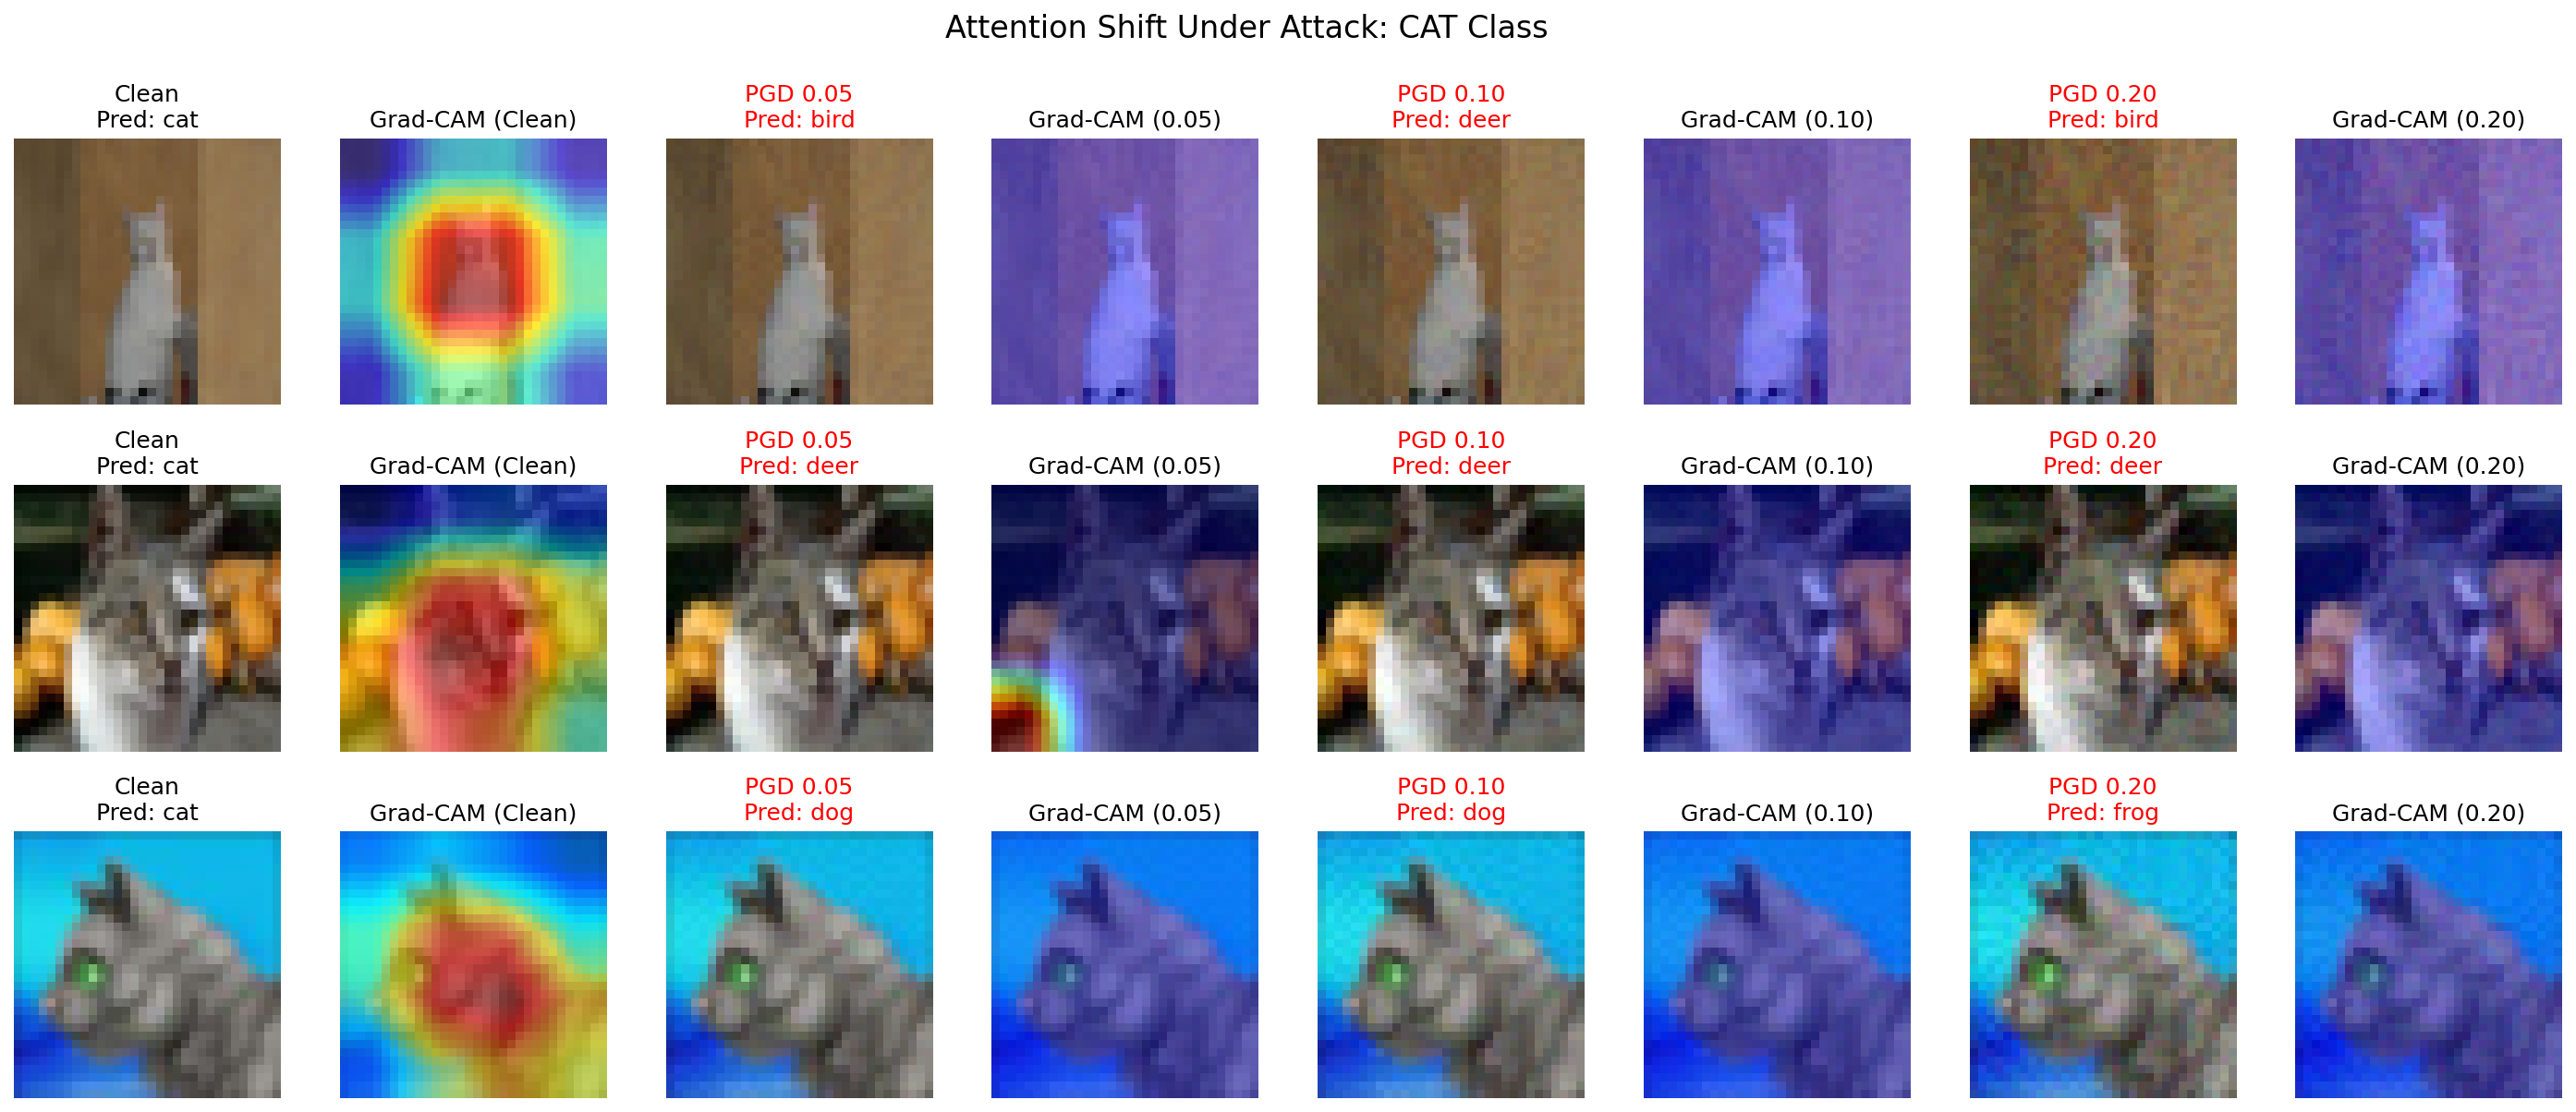
\includegraphics[width=\textwidth]{figures/cat_gradcam.png}
  \caption{Grad-CAM}
\end{subfigure}
\caption{\textbf{Cat Stimuli and Grad-CAM (Fig.~A.28, A.29)}.}
\end{figure}

\begin{figure}[H]
\centering
\begin{subfigure}[b]{0.32\textwidth}
  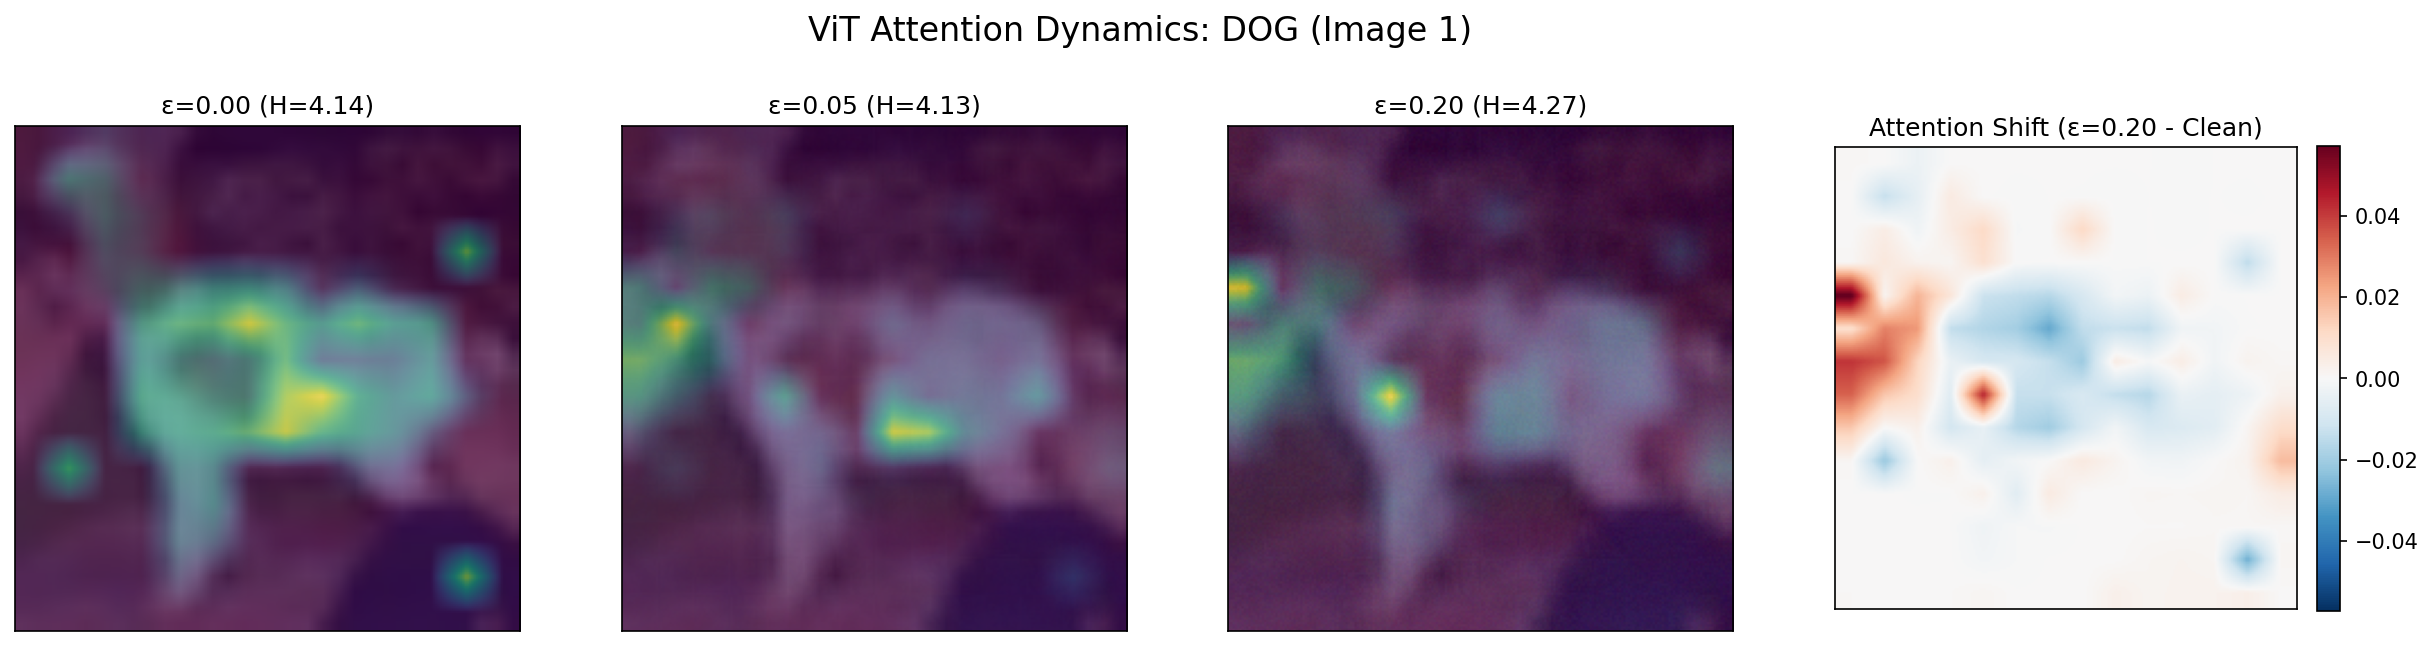
\includegraphics[width=\textwidth]{figures/dog_1.png}
  \caption{Clean}
\end{subfigure}
\hfill
\begin{subfigure}[b]{0.32\textwidth}
  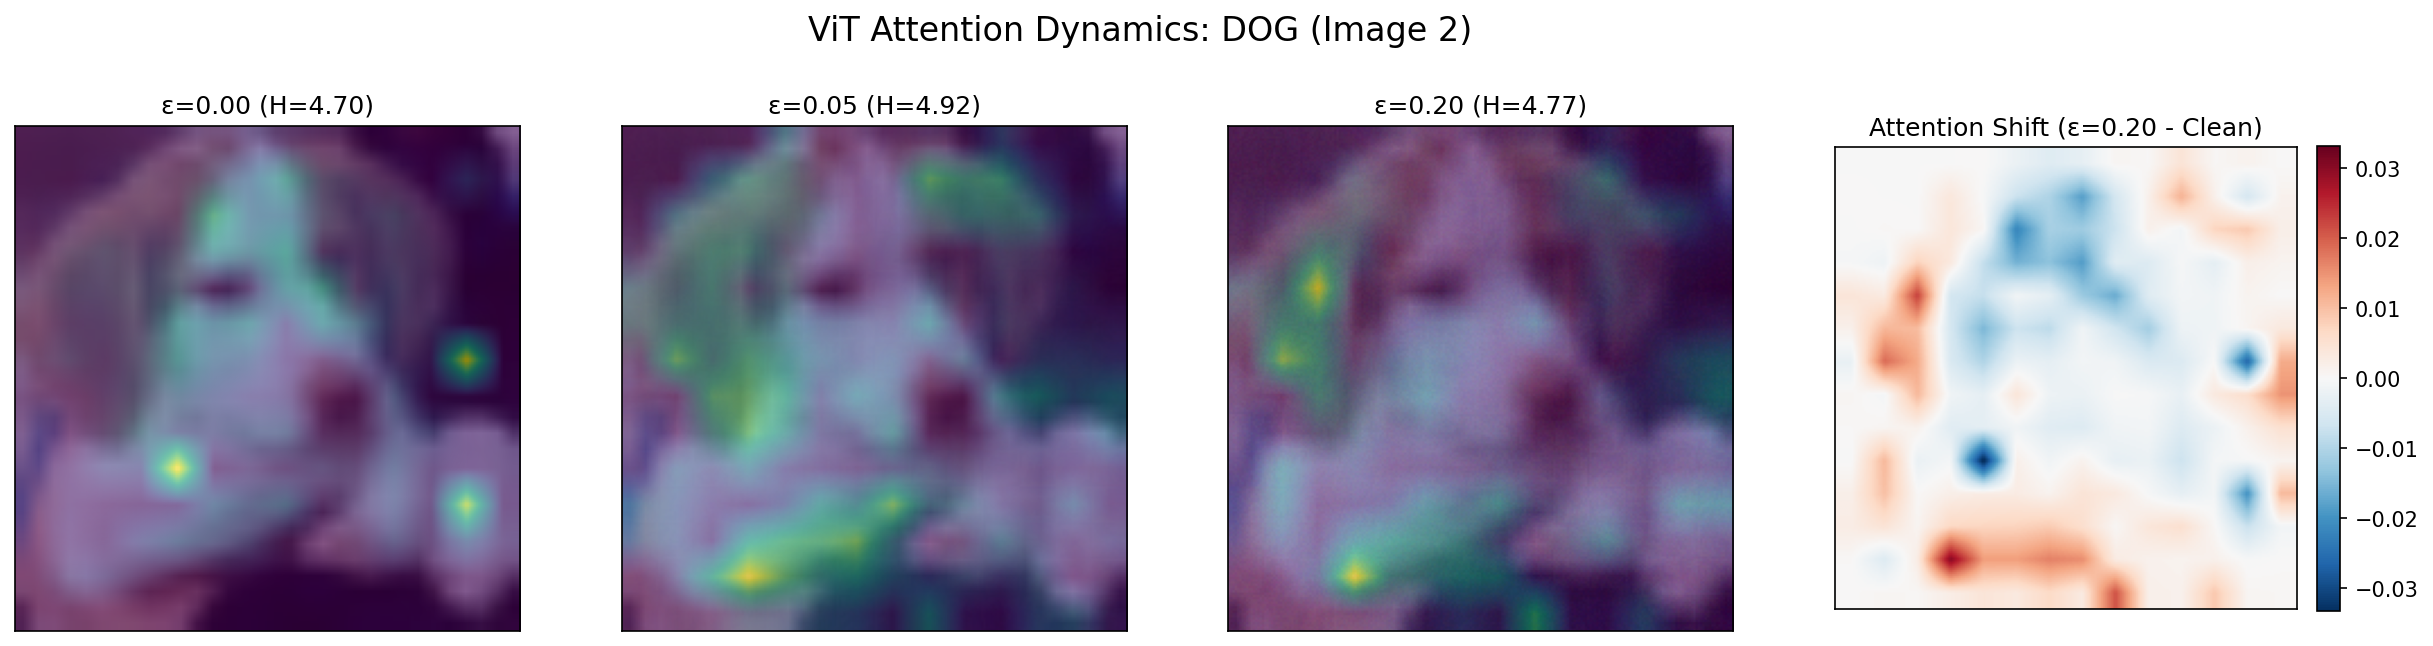
\includegraphics[width=\textwidth]{figures/dog_2.png}
  \caption{Adversarial}
\end{subfigure}
\hfill
\begin{subfigure}[b]{0.32\textwidth}
  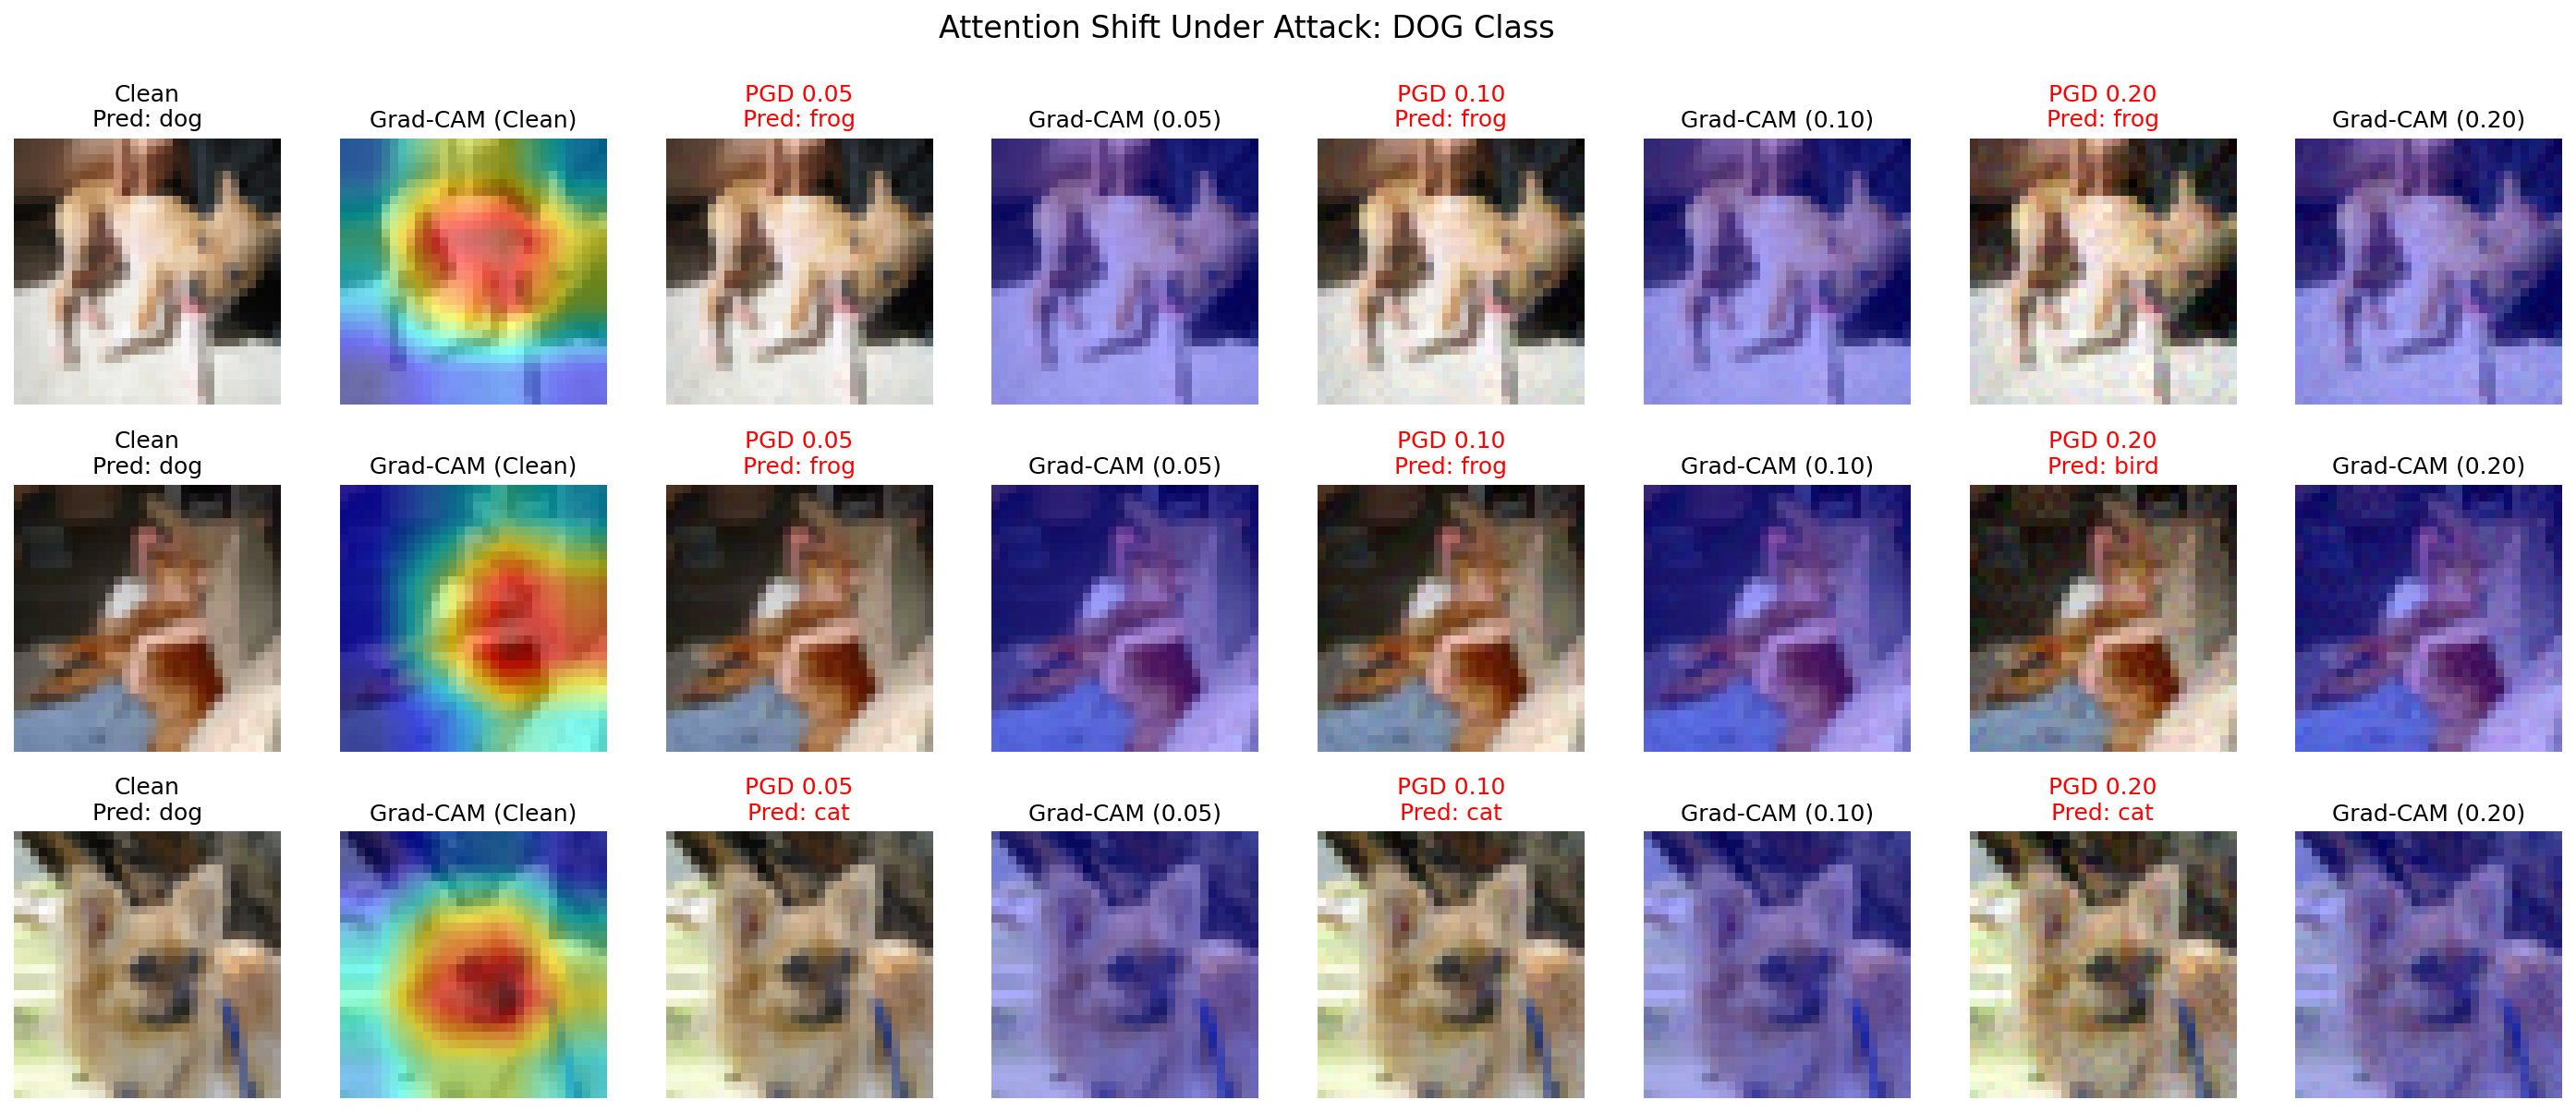
\includegraphics[width=\textwidth]{figures/dog_gradcam.png}
  \caption{Grad-CAM}
\end{subfigure}
\caption{\textbf{Dog Stimuli and Grad-CAM (Fig.~A.30, A.31)}.}
\end{figure}

\begin{figure}[H]
\centering
\begin{subfigure}[b]{0.32\textwidth}
  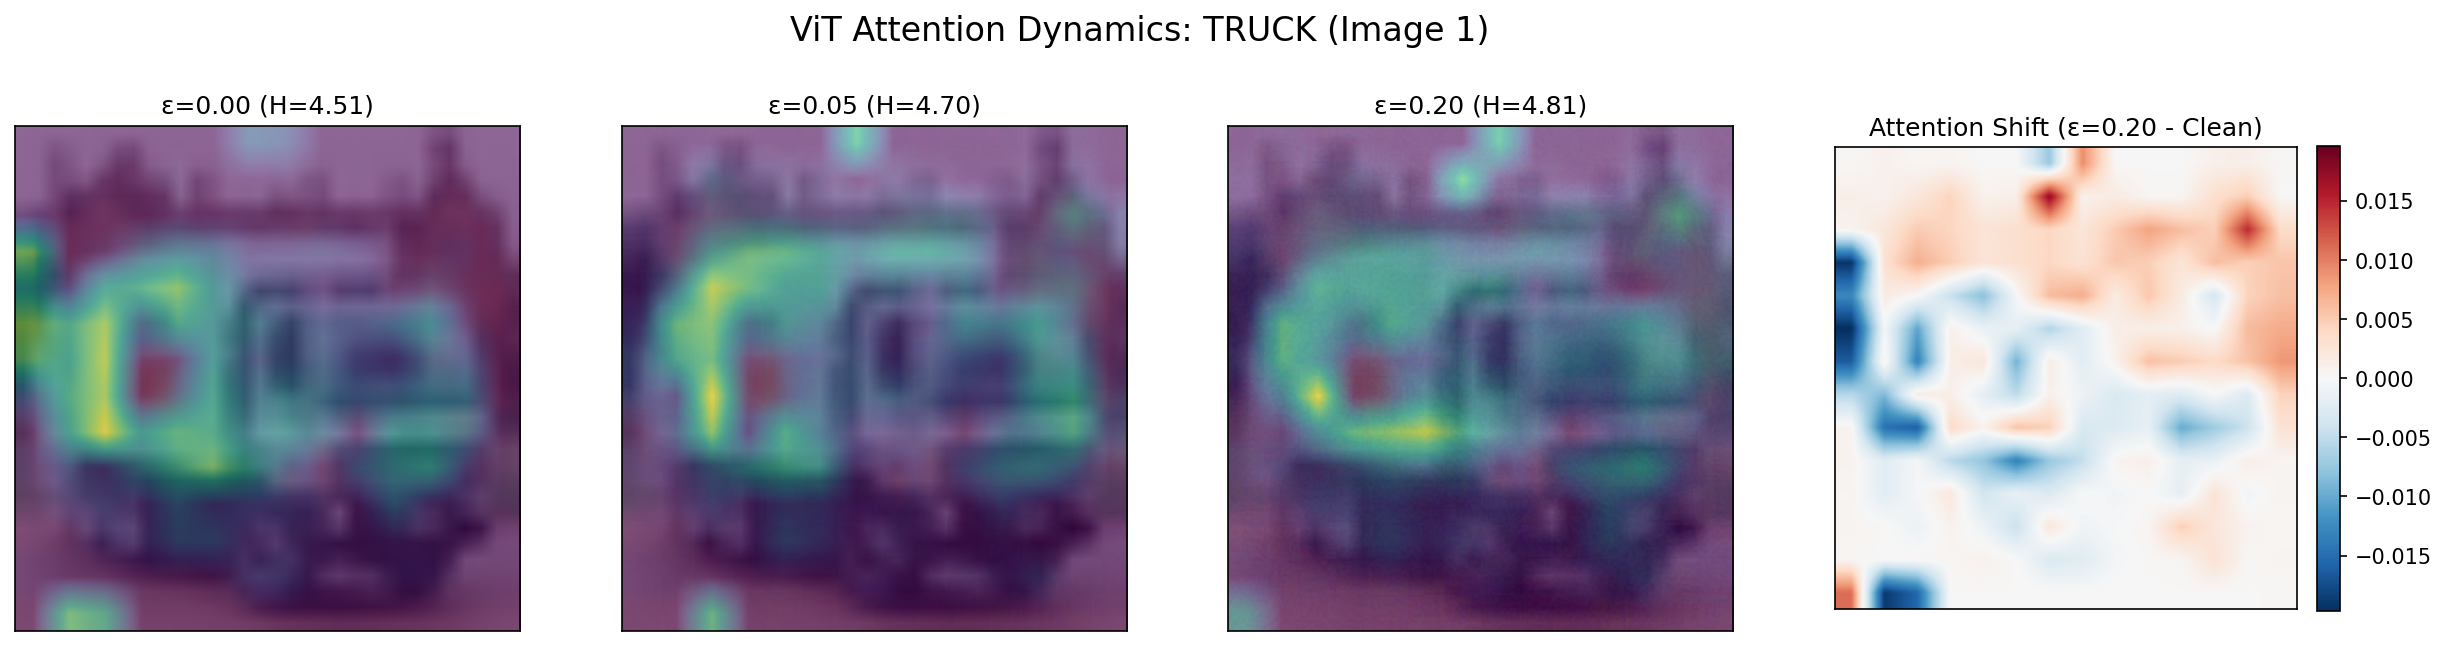
\includegraphics[width=\textwidth]{figures/truck_1.png}
  \caption{Clean}
\end{subfigure}
\hfill
\begin{subfigure}[b]{0.32\textwidth}
  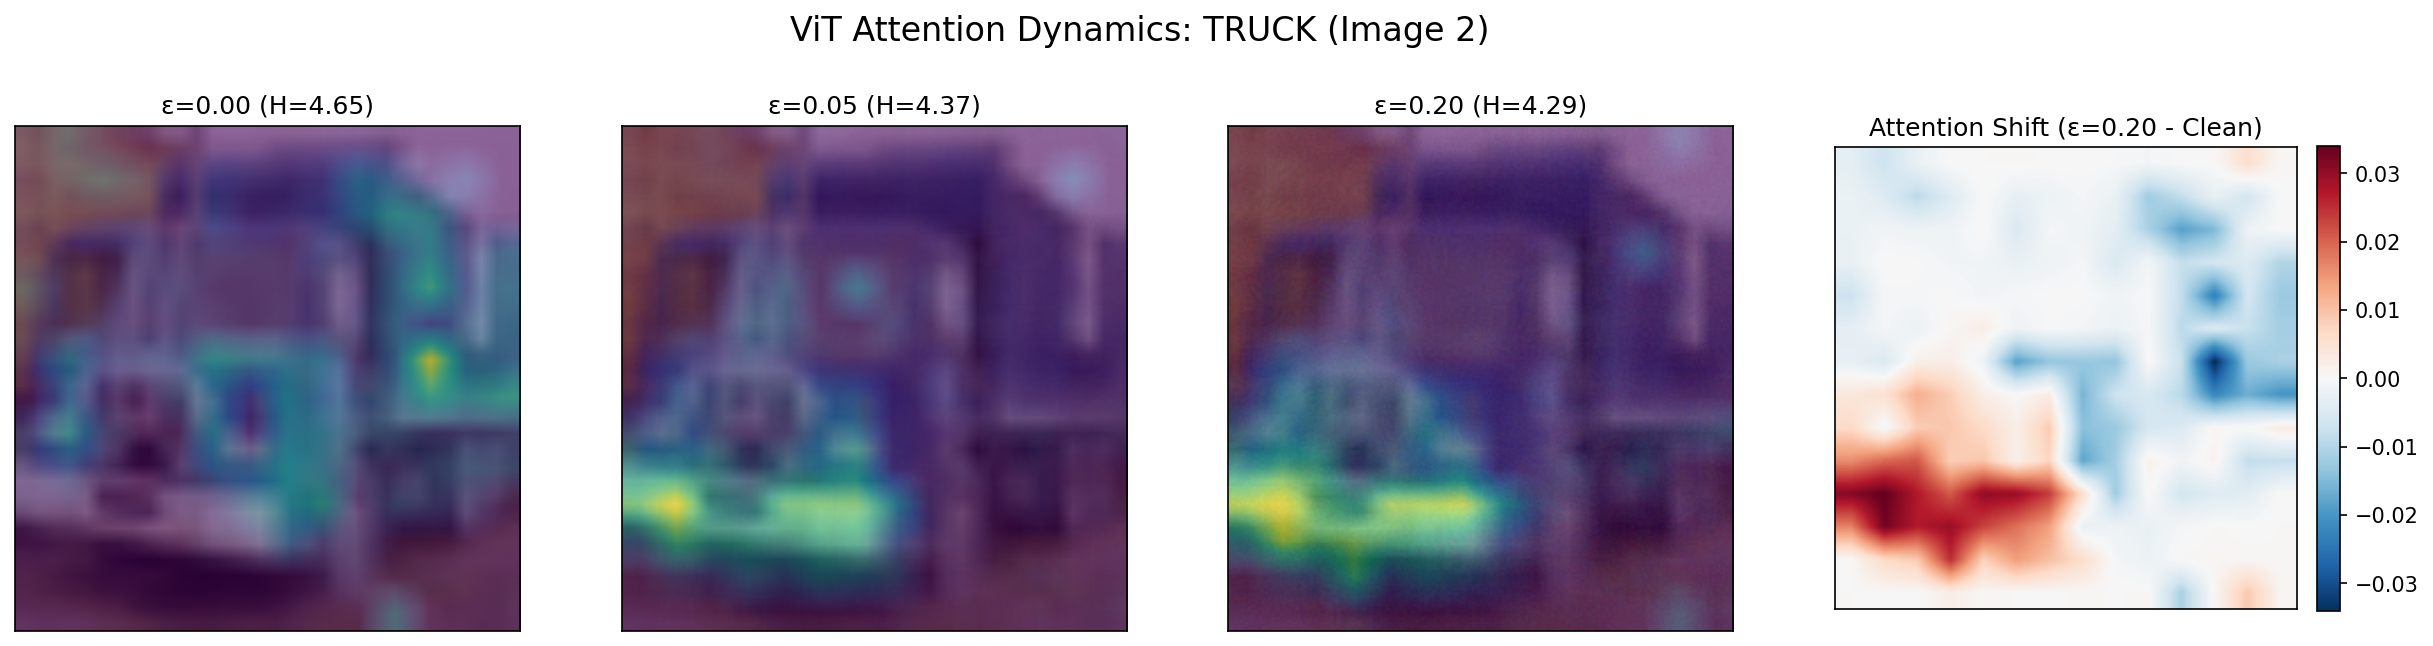
\includegraphics[width=\textwidth]{figures/truck_2.png}
  \caption{Adversarial}
\end{subfigure}
\hfill
\begin{subfigure}[b]{0.32\textwidth}
  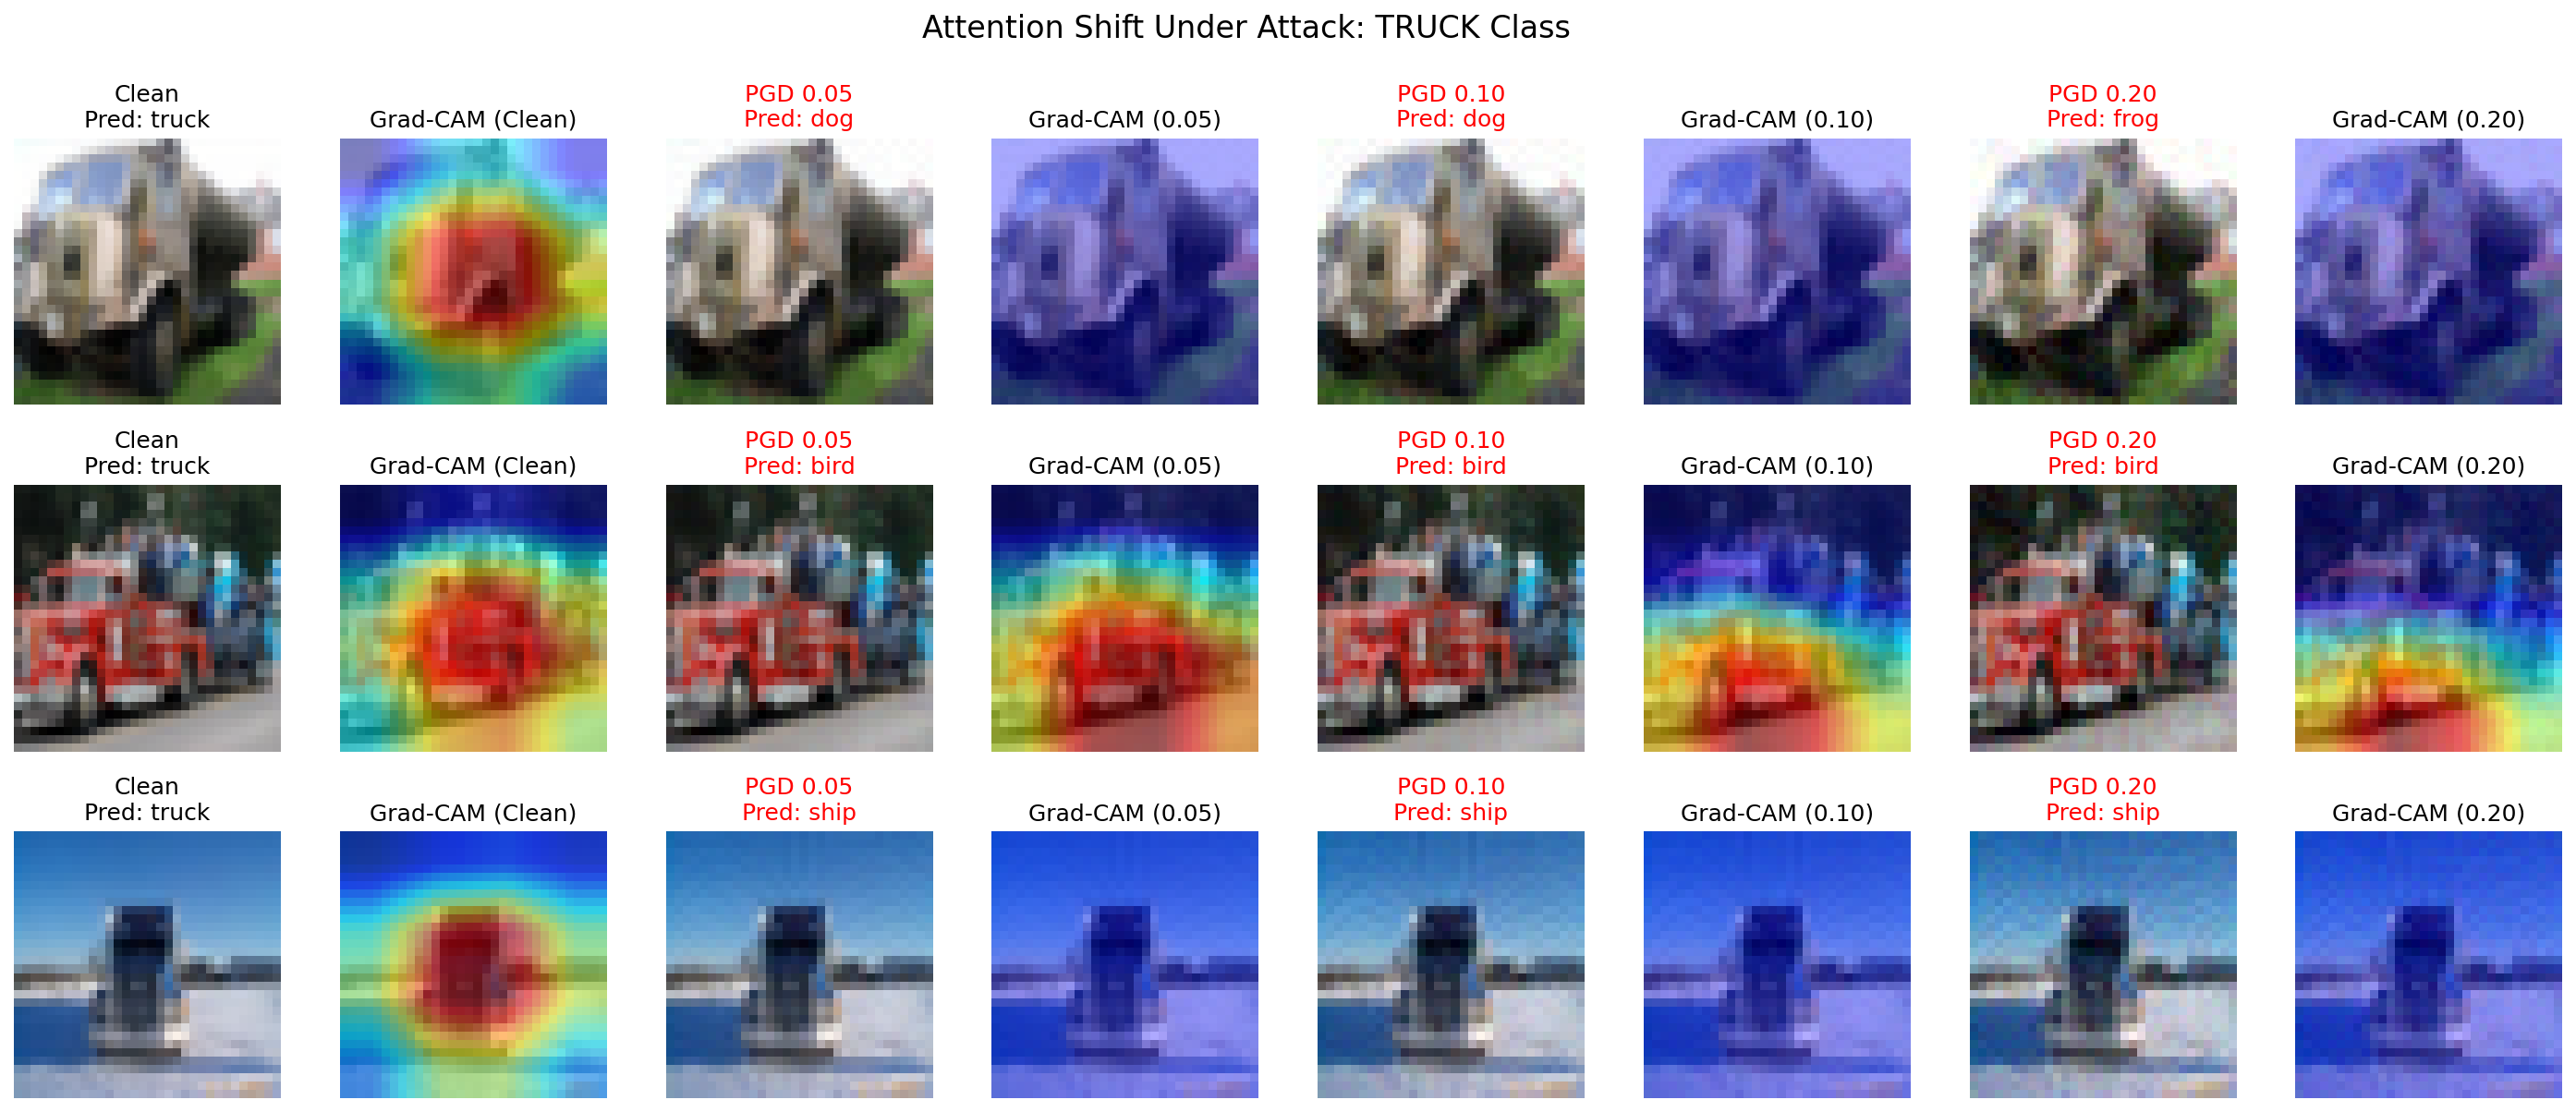
\includegraphics[width=\textwidth]{figures/truck_gradcam.png}
  \caption{Grad-CAM}
\end{subfigure}
\caption{\textbf{Truck Stimuli and Grad-CAM (Fig.~A.32, A.33)}.}
\end{figure}


% ============================================================
\section{Implementation Details}
\label{app:impl}
% ============================================================

\textbf{Hardware.}
Primary: NVIDIA RTX 4060 8\,GB VRAM, WSL2 Ubuntu 22.04.
Secondary: NVIDIA GTX 1650 2\,GB VRAM (Shape-ResNet training).
Cloud: Google Colab T4/L4 GPU instances (RHAN-Large STL-10 training).

\textbf{Software.}
Python 3.10, PyTorch 2.3 (CUDA 12.4), torchvision 0.18,
timm 0.9+, scikit-learn, scipy, numpy, matplotlib, seaborn.

\textbf{Memory management.}
Adversarial arrays use numpy memory-mapped arrays
(\texttt{mmap\_mode='r'}), batch size 64,
with \texttt{torch.cuda.empty\_cache()} between epsilon levels.

\textbf{Reproducibility.}
Random seeds fixed at 42. Code:
\url{https://github.com/FerrariKazu/Adversarial-Cognitive-Model}.

\end{document}
